%%%%%%%%%%%%%%%%%%%%%%%%%%%%%%%%%%%%%%%%%
% Arsclassica Article
% LaTeX Template
% Version 1.1 (10/6/14)
%
% This template has been downloaded from:
% http://www.LaTeXTemplates.com
%
% Original author:
% Lorenzo Pantieri (http://www.lorenzopantieri.net) with extensive modifications by:
% Vel (vel@latextemplates.com)
% Johan Bos (johan.bos@rug.nl)
% Barbara Plank (bapl@itu.dk)
% 
% License:
% CC BY-NC-SA 3.0 (http://creativecommons.org/licenses/by-nc-sa/3.0/)
%
%%%%%%%%%%%%%%%%%%%%%%%%%%%%%%%%%%%%%%%%%

%----------------------------------------------------------------------------------------
%	PACKAGES AND OTHER DOCUMENT CONFIGURATIONS
%----------------------------------------------------------------------------------------

\documentclass[
10pt, % Main document font size
a4paper, % Paper type
oneside, % One page layout (no page indentation)
headinclude,footinclude, % Extra spacing for the header and footer
%BCOR5mm, % Binding correction
] {book}%
\usepackage{eurosym}
\usepackage{makecell}
\usepackage{booktabs} % for nice tables with \toprule, \midrule
\usepackage{multicol}
\usepackage{changepage}
\usepackage{csvsimple,longtable}
\usepackage[utf8]{inputenc}
\setcounter{secnumdepth}{5}
\usepackage{adjustbox}
\usepackage{multirow}
\usepackage{caption}
\usepackage{geometry}
\usepackage{tcolorbox}
\usepackage{float}
\usepackage{changepage}
\usepackage{xcolor}
\usepackage[nottoc]{tocbibind}
\usepackage{fontawesome5}
\usepackage{subcaption}
\usepackage{tkz-euclide}
\usepackage{nameref}
\usepackage{glossaries}
\usepackage{makecell}
\usepackage{rotating}
\usepackage{chngcntr}
\newcounter{flowchart}
\usepackage{pgf}
\usepackage{url}
\usepackage{hyperref}
\usepackage{algorithm}
\usepackage{algpseudocode}
\usepackage{amsmath}
\usepackage{mdframed}
\usepackage{amsfonts}
\algrenewcommand\algorithmicrequire{\textbf{Input:}}
\algrenewcommand\algorithmicensure{\textbf{Output:}}

\input{extra/structure} % Include the structure.tex file which specified the document structure and layout


\usepackage{tikz}
\usepackage{tikz-network}
\usetikzlibrary{positioning}

\tikzstyle{process} = [
    rectangle,
    minimum width=3cm, minimum height=1cm,
    text width=3cm,
    draw=black!0, fill=orange!20,
    rounded corners,
    align=center
]


\tikzstyle{arrow} = [thick,->,>=stealth]

% http://mirrors.ibiblio.org/CTAN/graphics/pgf/contrib/tikz-network/tikz-network.pdf
\SetVertexStyle[Shape=circle, InnerSep=1, MinSize=3, FillColor=black, LineColor=black]
\SetEdgeStyle[Color=gray, Arrow=-stealth]

% \usetikzlibrary{external}
% \tikzexternalize[prefix=tikz/,optimize command away=\includepdf]


\usepackage{comment}


\usepackage{subcaption}

%----------------------------------------------------------------------------------------
%	HYPHENATION
%----------------------------------------------------------------------------------------

\hyphenation{Fortran hy-phen-ation} % Specify custom hyphenation points in words with dashes where you would like hyphenation to occur, or alternatively, don't put any dashes in a word to stop hyphenation altogether



%----------------------------------------------------------------------------------------
%	TITLE AND AUTHOR(S)
%----------------------------------------------------------------------------------------

\title{\normalfont\spacedallcaps{title}} % The article title

\author{\spacedlowsmallcaps{author}} % The article author(s) - author affiliations need to be specified in the AUTHOR AFFILIATIONS block

\date{} % An optional date to appear under the author(s)

%----------------------------------------------------------------------------------------


%----------------------------------------------------------------------------------------
%	GLOSSARY
%----------------------------------------------------------------------------------------
\makeglossaries
\newglossaryentry{stitch}{
    name={Stitch},
    description={A feature on TikTok that allows users to use a clip from another user's video and add their own response or continuation}
}

\newglossaryentry{duet}{
    name={Duet},
    description={A feature that lets users create a side-by-side video with another user's video, often for reactions, responses, or collaborations}
}

\newglossaryentry{comment}{
    name={Comment},
    description={A user response left on a video, allowing interaction and discussion between viewers and creators}
}

\newglossaryentry{video_reply}{
    name={Video Reply to Comment},
    description={A feature allowing creators to respond to a comment with a new video, linking the response directly to the original comment}
}

\newglossaryentry{algorithm}{
    name={Algorithm},
    description={TikTok's recommendation system, which curates content shown to users based on their interactions, preferences, and trends}
}

\newglossaryentry{trends}{
    name={Trends},
    description={Popular themes, challenges, or types of content that gain widespread attention on the platform}
}

\newglossaryentry{sounds}{
    name={Sounds/Use of Other’s Sound},
    description={Audio clips that users can borrow and use in their own videos, often leading to viral trends}
}

\newglossaryentry{hashtag}{
    name={Hashtag},
    description={Keywords preceded by a hash symbol (\#) that categorize and tag content, making it discoverable by users searching for specific themes or topics}
}

\newglossaryentry{captions}{
    name={Captions},
    description={Text added to videos by creators, providing context or commentary}
}

\newglossaryentry{descriptions}{
    name={Descriptions},
    description={Brief summaries or context provided in text under the video, often used to explain content or include hashtags. Descriptions are created by video creators upon uploading a video.}
}

\newglossaryentry{user}{
    name={User},
    description={An individual with an account on TikTok who can create, watch, and interact with videos}
}

\newglossaryentry{follower}{
    name={Follower},
    description={A user who has chosen to subscribe to another user's content, receiving updates and recommendations}
}

\newglossaryentry{FYP}{
    name={For You Page (FYP)}, 
    description={A personalized feed, where the shown videos are determined by the TikTok recommendation algorithm}
}


%----------

\begin{document}

%----------------------------------------------------------------------------------------
%	HEADERS
%----------------------------------------------------------------------------------------

%\renewcommand{\chaptermark}[1]{\markright{\spacedlowsmallcaps{#1}}} % The header for all pages (oneside) or for even pages (twoside)
%\renewcommand{\subsectionmark}[1]{\markright{\thesubsection~#1}} % Uncomment when using the twoside option - this modifies the header on odd pages
%\lehead{\mbox{\llap{\small\thepage\kern1em\color{halfgray} \vline}\color{halfgray}\hspace{0.5em}\rightmark\hfil}} % The header style

\pagestyle{scrheadings} % Enable the headers specified in this block


%----------------------------------------------------------------------------------------
%	TITLE PAGE
%----------------------------------------------------------------------------------------

\hypersetup{pageanchor=false}
\begin{titlepage}
\thispagestyle{empty}
\begin{figure}[h!] %  figure placement: here, top, bottom, or page
\centering
\includegraphics[width=4in]{extra/ITUlogo.jpg} 
\end{figure}

\begin{center}
\vspace{30 mm}
\begingroup \linespread{1,75} \selectfont 

% Title ideas
%\textsc{\LARGE What's on your wall?}\\
%\textsc{\Large Exploring communication on TikTok\\ through networks of stitches}\\[1,5cm]

% \textsc{\LARGE Characterizing communication patterns on TikTok through networks of stitches}\\


% \textsc{\LARGE StitchTok:}\\
\textsc{\LARGE TikTok StitchGraph:}\\
\textsc{\Large Characterizing communication patterns on TikTok through a collection of interaction networks}
% \textsc{\Large An exploration of TikTok stitches through a collection of interaction networks}
%\textsc{\Large Analyzing A Collection of Stitch-Based Interaction Networks to Characterize Communication}


% We like this 
%\textsc{\Large Characterizing communication patterns on TikTok through networks of stitches}\\

% Overtitel ide: "What do other data science students write their thesis about?"

\endgroup


\end{center}
\vfill
\textbf{Master's thesis}\\  %\textbf{Master thesis}\\
Data Science\\  
Mads Høgenhaug, Marcus Friis, Morten Pedersen\\
\\ 
\today\\
Supervisor: Luca Rossi
\end{titlepage}
\hypersetup{pageanchor=true}



%----------------------------------------------------------------------------------------
%	ABSTRACT
%----------------------------------------------------------------------------------------
\pagenumbering{roman}

\chapter*{Abstract}
\markboth{Abstract}{Abstract}
\addcontentsline{toc}{chapter}{Abstract}

We present TikTok StitchGraph: a collection of $36$ graphs based on TikTok stitches. With its rapid growth and widespread popularity, TikTok presents a compelling platform for study. Its recently introduced research API offers an opportunity to explore the intricacies of its content-remixing stitch feature. Leveraging this, in combination with web scraping, we construct graphs detailing stitch relations from both a video- and user-centric perspective. Specifically, we focus on user multi-digraphs, with vertices representing users and edges representing directed stitch relations. From the user graphs, we characterize common communication patterns of the stitch using frequent subgraph mining, finding a preference for stars and star-like structures, an aversion towards cyclic structures, and directional disposition favoring in- and out-stars over mixed-direction structures. These structures are augmented with sentiment labels in the form of edge attributes. However, the added complexity yields no new insights. Furthermore, no discovered subgraph is statistically significant under a configuration null model. Using these subgraphs for graph-level embeddings together with Graph2Vec, we show no clear distinction between topologies for different hashtag topic categories. Lastly, comparing StitchGraph to Twitter reply networks reveal no major findings with the subgraph analysis and graph embeddings. The dataset and methodology demonstrate one approach to comprising and analyzing network structures from TikTok.  

The complete codebase written to create the results for this paper is available in the project repository: \url{https://github.com/Marcus-Friis/thesis}

%chatty boy

%Write an abstract for this paper

% This study presents StitchTok, a novel dataset comprising 36 interaction graphs based on TikTok’s stitch functionality. By leveraging TikTok’s Research API and custom scraping pipelines, we constructed graphs reflecting user communication across diverse thematic hashtags. This dataset enables the examination of stitch-based communication patterns, addressing gaps in existing research on TikTok as a graph-structured platform. Our analysis explores topological features, sentiment dynamics, and motif patterns within the networks, comparing findings to analogous Twitter reply networks. Employing methods such as frequent subgraph mining, graph embeddings, and sentiment augmentation, we highlight characteristic interaction structures and thematic variations in TikTok stitches. Our findings reveal unique affordances of TikTok’s remix culture, providing foundational insights into short-form video communication and its implications for public discourse analysis.





%----------------------------------------------------------------------------------------
%	TABLE OF CONTENTS & LISTS OF FIGURES AND TABLES
%----------------------------------------------------------------------------------------
\clearpage
\setcounter{tocdepth}{3} % Set the depth of the table of contents to show sections and subsections only
\tableofcontents % Print the table of contents

%\listoffigures % Print the list of figures (optional, only if you have many figures)

%\listoftables % Print the list of tables (optional, only if you have many tables)

%\lstlistoflistings



%----------------------------------------------------------------------------------------
%	Preface
%----------------------------------------------------------------------------------------
\clearpage

\chapter*{Preface}
\markboth{Preface}{Preface}
\addcontentsline{toc}{chapter}{Preface}

This project has been a long journey, and throughout the process, we have received many helping hands. First and foremost, we would like to take this opportunity to thank Luca Rossi for being an absolutely outstanding supervisor on all accounts. Working together with him has been both highly educational and a genuine pleasure. We also extend our gratitude to Michele Coscia, for providing much needed support on the technicalities of frequent subgraph mining, Matteo Magnani and Alessia Galdeman, for providing valuable expert feedback on the project, and Marilena Hohmann, for sharing the Twitter data used in the project. 




%----------------------------------------------------------------------------------------
%	INTRODUCTION
%----------------------------------------------------------------------------------------
\clearpage
\pagenumbering{arabic}
\chapter{Introduction}

In the 21st century, the landscape of public discourse has undergone a significant transformation with the rise of short-form video content platforms such as TikTok, Instagram Reels, and YouTube Shorts.  Among these, TikTok has seen a significant increase in popularity, becoming one of the most popular social media services, with more than $1.67$ billion active monthly users worldwide \citep{tiktok_popular}. In particular, teens have heavily adopted this new format type \citep{tiktok_teens}. With the recent introduction of the TikTok Research API \citep{tiktokresearchapi}, performing large scale studies of TikTok has become a possibility. 

The short-form video format has been adopted for all communicative purposes, with content ranging from comedic sketches to serious political debates. This multifaceted nature of TikTok’s content makes it a compelling platform to study. The shift from traditional text-dominated social media, such as Facebook and X (formerly known as Twitter), to short-form video content presents new challenges in computationally analyzing public discourse. While natural language processing methods have sufficed for older platforms, the multimodal character of short-form video content introduces analytical challenges that require a combination of visual, auditory, and textual analysis.

TikTok has a plethora of social features. Among these is the \textit{stitch}. The stitch allows users to create a reactionary video of another video, incorporating up to five seconds of the \textit{stitched} video. Similarly, the \textit{duet} allows users to add their own video alongside another user's video in a split screen, floating head, or a green screen format. Unlike stitches, which integrate parts of the original video into the new content, duets display the original and new videos simultaneously and are not bound by the five second rule. This content remixing functionality yields an explicit network structure, where content can have direct connections to other content. This is akin to X's \textit{reply} and \textit{quote} functionality, where posts can be explicit reactions to other posts. Although there exists research on TikTok, most of it is qualitative, and almost no research focuses on studying TikTok as a graph. 

This paper presents TikTok StitchGraph: possibly the first graph dataset detailing stitches on TikTok. A stitch network is constructed comprising $36$ different hashtags, containing all stitches created in May $2024$ using one of said hashtags. The dataset aims to explore and improve understanding of how people communicate using stitches on TikTok. The topological structure of TikTok stitch networks and the content of individual videos are analyzed to uncover patterns and insights into this emerging form of public discourse. Additionally, these findings are compared to Twitter to highlight structural differences and commonalities in how users interact across these two social media platforms. The approach combines basic network analysis, sentiment analysis, frequent subgraph mining, and network embeddings to gain an introductory understanding of the stitch networks collected from TikTok. Specifically, this paper aims to answer the following research questions:

\begin{itemize}
    \item How can stitch communication on TikTok be studied through the lens of network analysis?
    \item What stitch patterns are characteristic of TikTok?
    \item How do the stitch patterns vary between different content themes on TikTok?
    \item How do the discovered properties of TikTok stitch networks compare with Twitter reply networks?
\end{itemize}


\section{An introduction to TikTok}
To understand the methods and findings of this paper, one must be familiar with TikTok as a platform and the dynamics that shape its content creation, consumption, and user interactions. This includes understanding the platform's algorithmic structure, the role of trends and challenges, and the unique ways users engage with and remix other users' content with stitches and duets. Throughout this section, multiple TikTok terms and concepts are introduced. For a complete overview, see the Appendix Glossary \ref{glossary}.

TikTok originated as the Chinese app \textit{Douyin}, launched internationally in $2017$. In $2018$, it merged with \textit{Musical.ly}, an app introduced in $2014$ for sharing lip-sync videos under one minute in length. By $2017$, Musical.ly had accumulated $200$ million users before being acquired and integrated into TikTok. This historical context shapes TikTok’s present-day culture, characterized by its demographic of young users and the popularity of dance videos, as well as the platform's distinctive features for video creation \citep{IJoC14543}.

Users consume TikTok through a personalized video feed, curated by TikTok's proprietary algorithm, commonly referred to as \textit{The Algorithm}. The algorithm pre-sents videos to users, and based on user engagement, it adapts the recommended content. This personalized video feed is known as the \textit{For You Page (FYP)} and is the main attraction of TikTok. Anyone can upload a video and have the algorithm show it in the feeds of other users. The algorithm has strict guidelines towards what content is allowed and will penalize any content that is not compliant with TikTok's policies. This has led users to mask content behind obscure internal ways of speaking and writing, leading to a phenomenon called \textit{algospeak} \citep{doi:10.1177/20563051231194586}. 


Other content remixing functionalities include \textit{duets}, \textit{video replies to comments}, and \textit{sound sync}. \textit{Duets} enable users to create collaborative videos in a side-by-side or picture-in-picture format, facilitating interaction through real-time reactions or joint performances. Similarly, \textit{video replies to comments} transform text-based feedback into engaging multimedia interactions. Lastly, \textit{sound sync} lets users create different videos based on the same sound, linking creators through shared auditory elements. These features collectively contribute to an active and creative environment, where users can remix content and interact in different ways. However, by design of the 'For You Page', the exact content being interacted with is heavily influenced by what the algorithm recommends.

% For this study, we focus only on stitches to maintain a clear direction and avoid becoming overwhelmed by the vast range of interaction types on TikTok. Although duets and other forms of video replies offer valuable insights, the volume of data could make the analysis too complex. By narrowing our scope to stitches, we ensure that we can thoroughly explore the dynamics within this specific feature without losing focus. Additionally, there are more than enough data from stitches alone to provide a comprehensive view of communication patterns on TikTok. 
TikTok offers a variety of interactive features that shape the way users interact and create content. One of the key features is \textit{hashtags}, which serve as markers for different topics and communities, helping users find and engage with specific content. However, beyond hashtags, TikTok introduced the \textit{stitch} feature in $2020$, adding a new layer to communication \citep{introducingStitch}. This stitch feature is commonly used to create video reactions to other content. Importantly, users cannot stitch a video that is already a stitch of another video. TikTok also gives users control over this feature, allowing them to disable stitching for specific videos or for all of their content. When a video is stitched, the description will show “stitch with @username” and, most of the time\footnote{We have observed that some users remove the hyperlink from the video description, rendering us unable identify the stitched video.}, provide a direct link to the original video. Throughout this paper, we refer to the user creating the stitch as the "\textit{stitcher}" and the user whose video is being stitched as the "\textit{stitchee}".

\label{Intro}

% In this study, we take a network-centric approach to understand the use of TikTok stitches. 


% TODO

% motivation

% research question(s)

% \section{TikTok}

TikTok is a global video sharing service released in 2016, quickly growing to become the most popular app in 2019 and 2020, now having more than a billion users. The main way to use it is via a personalized video feed, showing generally short vertical videos. Anyone can upload a video and have the algorithm show it in other users feeds. TikTok earns money mainly by showing commercials in the form of paid videos in feeds, and users are paid by views or external ways like sponsors and merchandise.
TikTok history, started with music.. impacts the culture and functionality today
No of users, videos and so on
Research API, launched in 2023 not including data from users under 18, Canada, and private content. 
Userbase demographics
Niche and TikTok specific communities


% \begin{center}
% \begin{minipage}{0.9\textwidth}  % Adjust width as needed
%     \renewcommand{\glossaryname}{Glossary of TikTok Terms}
%     \glsaddallunused
%     \Small
%     \printglossaries
% \end{minipage}
% \end{center}


% \section{Communication on TikTok}
TikTok offers a range of interactive features that shape how users communicate on the platform. One of the key features is hashtags, which serve as markers for different topics and communities, helping users find and engage with specific content. However, beyond hashtags, TikTok introduced the stitch feature in 2020, adding a new layer to communication. A stitch allows users to respond to another video by incorporating a clip from the original video, but only up to five seconds. Importantly, users cannot stitch a video that is already a stitch of another video, which creates a limitation in the communication structure, often leading to dyads or star-like topologies in the user interaction graph. TikTok also gives users control over this feature, allowing them to disable stitching either for specific videos or across all their content. When a video is stitched, the description will show “stitch with @username” and, most of the time\footnote{We have made a few observations that some accounts have removed the hyperlink from the title, rendering us unable to be redirected to the stitched video}, provide a direct link to the original video. \\

In addition to stitching, TikTok allows users to reply to videos in comments. Interestingly, users can also respond to comments with videos, further blurring the line between text and video-based communication. The duet feature, another popular form of interaction, allows users to create a side-by-side or picture-in-picture collaboration, making it perfect for real-time reactions or joint performances. Another key communication feature is the use of original sound or music\_id, where users borrow audio from other videos\citep{tiktok_features}. This creates a sound-based network, linking different videos and users through shared audio, fostering connections and interactions across the platform.

TikTok’s features like stitches, duets, comments, and original sounds all help create an active and creative environment where users can interact in different ways. However, how they use these features is influenced by the platform’s design and algorithm, which affect what content gets seen and shared.

For this study, we focus only on stitches to maintain a clear direction and avoid becoming overwhelmed by the vast range of interaction types on TikTok. While duets and other forms of video replies offer valuable insights, the volume of data could make the analysis too complex. By narrowing our scope to stitches, we ensure that we can thoroughly explore the dynamics within this specific feature without losing focus. Additionally, there is more than enough data from stitches alone to provide a comprehensive view of communication patterns on TikTok. 





\clearpage

\chapter{Background}

This paper collects data for and quantitatively analyzes communication on TikTok. While qualitative methods and ethical considerations regarding TikTok have been fairly well documented, quantitative studies of communication on the platform remain scarce. For this reason, we also look towards similar social network studies conducted on Twitter, leveraging its similarities as a platform to further our understanding of TikTok.


\section{Research on TikTok}

The digital age has transformed how people engage with the media, moving from passive consumption to active participation. This shift has led to the growth of online communities, where users create and share their own content. This is known as participatory culture, where users are both consumers and creators of media \citep{jenkins2015participatory}. On platforms like TikTok, features such as stitching and duets enable users to remix and share videos, allowing trends and ideas to spread rapidly. The concept of "produsage" describes how users continuously build on and adapt existing content \citep{bruns2008blogs}.

TikTok’s stitching feature illustrates this by allowing users to incorporate parts of other videos into their own, blending the roles of creator and consumer \citep{tiktok_stitch_2020}. This creates an environment where content evolves through collaboration. As \cite{kaur2022customization} shows, TikTok also allows marginalized communities, such as migrant workers in Singapore, to document their poor experiences and challenge the mainstream narratives. Using TikTok's remix features, these workers engage in digital activism, bringing visibility to their unstable living conditions during the pandemic. This aligns with the concept of produsage, where users not only consume content but actively create and remix it, increasing internet exposure for underrepresented voices.

Although these participatory characteristics foster collaboration and community, they also raise legal and ethical questions. According to \cite{ripplexn2023stitch}, TikTok’s stitch function enables users to engage with existing content in ways that promote viral trends, but also introduces concerns regarding intellectual property. Users must navigate complex questions of content ownership and copyright, as the remixing culture enabled by stitches often blurs the line between original creation and derived work.

Similarly, the internet makes it easy for groups to form and collaborate without formal structures, allowing communities to emerge around shared interests \citep{shirky2008here}. On TikTok, these communities often form around hashtags, challenges, trends, and interactions. For this study, understanding these patterns is key as we explore how TikTok’s stitching feature influences communication. The way users engage through stitching aligns with the ideas of \cite{jenkins2015participatory}, \cite{bruns2008blogs}, and \cite{shirky2008here}, creating a space where users build on each other’s content and communities grow organically.

Although the role of features such as stitches in content creation has been acknowledged, there has been limited research specifically analyzing how these functions contribute to broader trends and connections within the TikTok ecosystem. In a systematic review of TikTok research, \cite{tiktok_review} found that most of the early TikTok studies used content analysis methods and focused on topics such as user behavior and platform governance. However, they noted significant gaps in research that looks into the unique capabilities of TikTok features, including tools like stitches and duets. This oversight underlines the need for studies such as ours, which aim to investigate how TikTok videos, particularly those using the stitching feature, form interconnected networks of content creation. To bridge this gap, researchers can now use TikTok’s research API to gather data at scale. The API provides a structured means of collecting information on videos, user engagement, and interactions, offering researchers a more systematic approach to analyzing TikTok’s various data. 

However, while the API opens up new opportunities for large-scale analyses, it also presents several notable limitations. As \cite{corso2024we} found, the API frequently fails to deliver the full quota of requested data, with researchers often receiving only $65\%$ of the expected content. This issue is made worse because it is unclear when and why some data is missing, especially with older videos that might have been deleted or set to private. 

%Furthermore, the API tends to over-represent certain geographic regions, particularly Asia, creating biases in the data that can skew results. These shortcomings highlight the challenges of relying solely on the API for comprehensive studies of TikTok’s global content network.

Despite these issues, the TikTok Research API remains a valuable tool for capturing large datasets that were previously inaccessible, and it allows for the examination of features like stitches in more detail than traditional methods. Using this API, this study aims to explore the connections between stitched videos and the broader content networks they form, addressing some of the gaps in understanding how TikTok’s unique affordances shape user interaction and content remixing.



\section{Previous Analyses of Social Networks}
% Communication networks are not exclusive to TikTok; they are a fundamental feature of many social media platforms, including Twitter\footnote{In this section, we refer to the platform as Twitter, as this was its name at the time of the studies cited. While the platform is now known as X, this distinction maintains historical consistency with prior research}. These platforms enable users to interact through explicit or implicit connections, forming complex networks that reveal patterns of communication, influence, and content propagation. For example, on Twitter, the retweet graph captures the relationships between users who share each other's posts, offering a structured way to study how information spreads and how users engage with content \citep{bild2015aggregate}. This concept closely parallels TikTok's stitch network, where users remix or respond to videos, creating a similar structure of communication.
Social networks have been widely studied, especially on platforms like Twitter\footnote{In this section, we use the name Twitter to match the platform’s name at the time of the studies mentioned. Although now called X, this helps maintain consistency with previous research.}, which has been a key focus for analyzing how people communicate online. These platforms allow users to interact through direct or indirect connections, forming networks that show patterns of communication, influence, and how content spreads. Twitter’s features, like retweets and replies, create clear links between users and their posts, making it easier to study how information flows. For example, a retweet graph maps the connections between users sharing each other’s posts, providing a way to analyze how content spreads \citep{bild2015aggregate}.

Research on Twitter has looked at many aspects of communication, such as political influence, user behavior, and network structures. \citet{torregrosa2020analyzing} demonstrate how relevance and centrality within a Twitter network correlate with the spread of extremist discourse, emphasizing that the role of influential users helps shape the flow of content. \citet{lassen2011twitter} examine how politicians use the unique features of Twitter to reach their audiences, finding that these features shape communication styles and visibility. \citet{doi:10.1126/sciadv.abq2044} explore polarization on the platform, showing how ideological divides and network clustering create echo chambers. Since networks play such a key role in understanding social media, studying similar patterns on other platforms is important. 

TikTok’s stitch feature provides a way to study communication through explicit connections, similar to how Twitter retweet networks have been analyzed. For instance, studies like \cite{garimella2018political} used Twitter data to model retweet graphs and examine interaction patterns around political events. 

Graph theory is an essential tool for studying these communication networks. Metrics such as centrality help identify key users or videos, while community detection reveals clusters of related activity. For example, analyses of Twitter retweet graphs by \cite{doi:10.1073/pnas.2023301118} have demonstrated how interactions often lead to clusters of like-minded users, sometimes forming echo chambers. Although our study does not focus on polarization or ideological alignment, we use similar techniques, such as centrality metrics to highlight influential nodes, and graph structure analysis to examine topological patterns. 

Datasets from Twitter, such as the "Coronavirus Tweet Ids" dataset \citep{kerchner2020coronavirus}, provide useful points of comparison. These datasets capture explicit user interactions, such as retweets and replies, which align closely with the stitched relationships in TikTok networks. Although the two platforms differ in format and features, their structural similarities enable direct comparisons through graph analysis. 

Prior social network research has focused heavily on Twitter. In this paper, we apply some of the presented methodologies to a newly composed TikTok stitch graph, while in parallel relating the findings to Twitter reply networks from \cite{doi:10.1126/sciadv.abq2044}. By conducting this analysis, we extend insights from Twitter studies to TikTok, addressing gaps in understanding its unique communication dynamics.  

\chapter{Data \& Material}

Our main contribution is composing the TikTok StitchGraph dataset. The dataset consists of stitch videos with metadata, such as user, views, hashtags, etc., and stitch relations between videos. All stitches using one of $36$ selected hashtags are collected for all videos created in May $2024$. For a video to be included in the dataset, it must be a stitch or a video being stitched. Along with the base TikTok stitch graph dataset, we enrich the data with video transcriptions, detected languages, audio content type, and transcription sentiments. The result is a dataset composed of $36$ different graphs, with video metadata and audio data. These can be used in two ways; as \textbf{a) video graphs} and \textbf{b) user graphs}. 


\begin{figure}[H]
    \centering
    \begin{subfigure}{0.5\textwidth}
        \centering
        \SetVertexStyle[Shape=circle, InnerSep=2, MinSize=14, FillColor=orange!40, LineColor=black, TextFont=\normalsize]
\SetEdgeStyle[Color=gray, Arrow=-stealth]

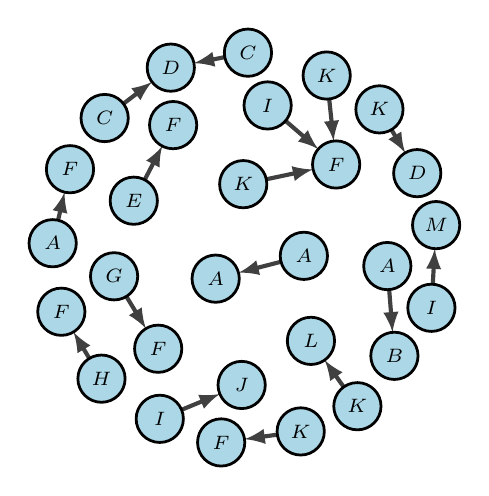
\begin{tikzpicture}
	\Vertex[x=-0.03, y=-0.88, label=$A$]{0}
	\Vertex[x=-1.15, y=-1.17, label=$A$]{1}
	\Vertex[x=1.03, y=-1.01, label=$A$]{2}
	\Vertex[x=1.12, y=-2.15, label=$B$]{3}
	\Vertex[x=-0.74, y=1.70, label=$C$]{4}
	\Vertex[x=-1.72, y=1.51, label=$D$]{5}
	\Vertex[x=-2.56, y=0.87, label=$C$]{6}
	\Vertex[x=-2.19, y=-0.18, label=$E$]{7}
	\Vertex[x=-1.69, y=0.78, label=$F$]{8}
	\Vertex[x=-3.22, y=-0.72, label=$A$]{9}
	\Vertex[x=-3.00, y=0.22, label=$F$]{10}
	\Vertex[x=-2.44, y=-1.14, label=$G$]{11}
	\Vertex[x=-1.88, y=-2.06, label=$F$]{12}
	\Vertex[x=-2.60, y=-2.44, label=$H$]{13}
	\Vertex[x=-3.11, y=-1.59, label=$F$]{14}
	\Vertex[x=-1.86, y=-2.95, label=$I$]{15}
	\Vertex[x=-0.82, y=-2.52, label=$J$]{16}
	\Vertex[x=0.65, y=-2.79, label=$K$]{17}
	\Vertex[x=0.06, y=-1.96, label=$L$]{18}
	\Vertex[x=-0.07, y=-3.11, label=$K$]{19}
	\Vertex[x=-1.08, y=-3.25, label=$F$]{20}
	\Vertex[x=-0.80, y=0.03, label=$K$]{21}
	\Vertex[x=0.38, y=0.28, label=$F$]{22}
	\Vertex[x=0.26, y=1.41, label=$K$]{23}
	\Vertex[x=0.93, y=0.98, label=$K$]{24}
	\Vertex[x=1.41, y=0.17, label=$D$]{25}
	\Vertex[x=-0.49, y=1.03, label=$I$]{26}
	\Vertex[x=1.59, y=-1.54, label=$I$]{27}
	\Vertex[x=1.65, y=-0.49, label=$M$]{28}
	\Edge[Direct](0)(1)
	\Edge[Direct](2)(3)
	\Edge[Direct](4)(5)
	\Edge[Direct](6)(5)
	\Edge[Direct](7)(8)
	\Edge[Direct](9)(10)
	\Edge[Direct](11)(12)
	\Edge[Direct](13)(14)
	\Edge[Direct](15)(16)
	\Edge[Direct](17)(18)
	\Edge[Direct](19)(20)
	\Edge[Direct](21)(22)
	\Edge[Direct](23)(22)
	\Edge[Direct](24)(25)
	\Edge[Direct](26)(22)
	\Edge[Direct](27)(28)
\end{tikzpicture}



        \caption{Video graph}
        \label{fig:biden_vgraph}
    \end{subfigure}%
    \begin{subfigure}{0.5\textwidth}
        \centering
        \SetVertexStyle[Shape=circle, InnerSep=2, MinSize=14, FillColor=orange!40, LineColor=black, TextFont=\normalsize]
\SetEdgeStyle[Color=gray, Arrow=-stealth]


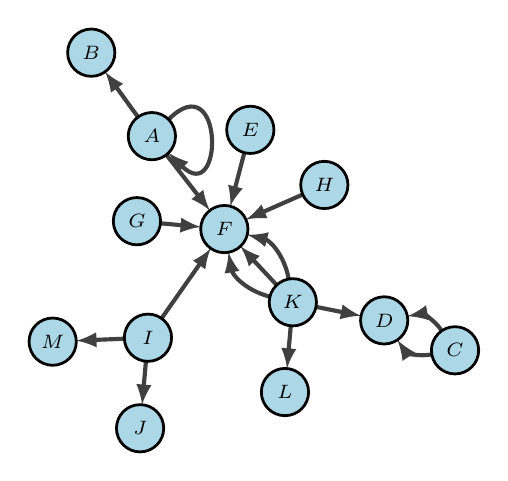
\begin{tikzpicture}
	\Vertex[x=-0.85, y=1.59, label=$A$]{0}
	\Vertex[x=-1.62, y=2.65, label=$B$]{1}
	\Vertex[x=3.00, y=-1.13, label=$C$]{2}
	\Vertex[x=2.1, y=-0.75, label=$D$]{3}
	\Vertex[x=0.40, y=1.67, label=$E$]{4}
	\Vertex[x=0.07, y=0.41, label=$F$]{5}
	\Vertex[x=-1.04, y=0.51, label=$G$]{6}
	\Vertex[x=1.34, y=0.97, label=$H$]{7}
	\Vertex[x=-0.9, y=-0.97, label=$I$]{8}
	\Vertex[x=-1, y=-2.12, label=$J$]{9}
	\Vertex[x=0.94, y=-0.52, label=$K$]{10}
	\Vertex[x=0.84, y=-1.66, label=$L$]{11}
	\Vertex[x=-2.11, y=-1.02, label=$M$]{12}
	\Edge[Direct](0)(0)
	\Edge[Direct](0)(1)
	\Edge[Direct, bend=-33](2)(3)
	\Edge[Direct, bend=33](2)(3)
	\Edge[Direct](4)(5)
	\Edge[Direct](0)(5)
	\Edge[Direct](6)(5)
	\Edge[Direct](7)(5)
	\Edge[Direct](8)(9)
	\Edge[Direct](10)(11)
	\Edge[Direct](10)(5)
	\Edge[Direct, bend=-33](10)(5)
	\Edge[Direct, bend=33](10)(5)
	\Edge[Direct](10)(3)
	\Edge[Direct](8)(5)
	\Edge[Direct](8)(12)
\end{tikzpicture}

        \caption{User graph}
        \label{fig:biden_ugraph}
    \end{subfigure}
    \caption{Example user- and video graph, created from a sample of \textit{\#biden2024}. Letters denote the user affiliated with the vertex. Video graphs are digraphs, where each vertex is a video and an edge is a stitch relation. They consist solely of stars, with edges being directed towards the central vertex. User graphs are multi-digraphs, where each vertex is a user and each edge is a stitch relation. In user graphs, all patterns can exists including self loops and multiedges.}
    \label{fig:biden}
\end{figure}

\textbf{a) Video graphs} are digraphs $G_v=(V,E)$, where vertices are TikTok videos, and edges are directed stitch relations. If video $u$ (the stitcher) stitches video $v$ (the stitchee), there is a directed edge $\{u, v\}$. The affordances and constraints of TikTok dictate the shape that video graphs can take. All video graphs consist of one or multiple stars $S_k$ ranging in size between a dyad $S_1$, and full star graph $S_{|E|}$, with the directionality always pointing towards the central vertex in the stars. This means that the number of edges $|E|$ for any video graph will range between $\frac{|V|}{2}$ and $|V| - 1$. The number is minimized when the graph consists entirely of dyads $S_1$, and maximized when the entire graph is a star $S_{|E|}$.

\textbf{b) User graphs} are multi-digraphs $G_u=(V,E)$, where vertices are users, and edges are stitch relations, but between users who stitch each other's videos. If user $u$ stitches a video from user $v$, then there is a directed edge $\{u,v\}$. Since users can create multiple stitches and be stitched multiple times, the topology of user graphs is not as rigid as that of video graphs. It allows for any arbitrary shapes along with self loops, since users can stitch videos from themselves, and multi-edges, since users can create multiple stitches of a video or different videos from another user. The size of the user graph is constrained by its respective video graph. The number of vertices in the user graph $|V_u|$ ranges from $1$ to the number of vertices in the video graph $|V_v|$, depending on the number of unique video creators. The number of edges for both the user- and video graph will always be equivalent $|E_u| = |E_v|$. 




\section{Data Collection}
To compose the TikTok StitcGraph dataset, we use \textit{TikTok's Research API} \citep{tiktokresearchapi} and web scraping. Through the API, we collect video metadata. Formally, the only requirement for querying the API is a time period. However, due to API instability\footnote{Note that the API instability heavily constrained the possibilities for the project, and any query too large would crash the API with error \texttt{500 Internal Server Error}.}, we found it helpful to constrain requests further, as it led to more stable API behavior. The API supports filtering by \texttt{"create\_date"}, \texttt{"username"}, \texttt{"region\_code"}, \texttt{"video\_id"}, \texttt{"hashtag\_name"}, \texttt{"keyword"}, \texttt{"music\_id"}, \texttt{"effect\_id"}, and \texttt{"video\_length"}. To compose this dataset, we filter by \texttt{"hashtag\_name"} and \texttt{"keyword"} (the video description).

The API is limited with regards to stitches, as it does not have any native functionality for querying stitches or getting stitch relations\footnote{This is not true as of November $2024$. A field called \texttt{video\_mention\_list} has been added to the API, which contains a list of users tagged in a video. However, when we did the project, this feature did not exist.}. However, when a stitch is created, TikTok will automatically put "\#stitch with @\textit{username}" in the video description along with a hyperlink to the stitched video. The hyperlink to the stitchee is only available on the TikTok website or app and not through the API. This means that we cannot create the desired network purely through the API. Instead, we need to use a combination of API requests and web scraping to collect the data. The result is the following three-step pipeline: querying stitch video metadata through the API, scraping the IDs of videos being stitched from TikTok's website, and querying the API for the metadata of the stitched videos. The collection process is repeated for each of the $36$ selected hashtags for May $2024$. This process is seen in Figure \ref{fig:data_flowchart}.


\begin{figure}[H]
    \centering
    \begin{adjustwidth}{-\textwidth}{-\textwidth} % Adjust the values as needed
        \centering
        \SetVertexStyle[Shape=circle, InnerSep=2, MinSize=8, FillColor=orange!40, LineColor=black]
\SetEdgeStyle[Color=gray, Arrow=-stealth]

\tikzstyle{query} = [
    rectangle,
    minimum width=4cm, minimum height=1cm,
    text width=3.8cm,
    draw=black!0, 
    fill=gray!20,
    rounded corners,
    align=center
    % font=\normalfont
]

\tikzstyle{hashtags} = [
    rectangle,
    minimum width=2cm, minimum height=1cm,
    text width=2cm,
    draw=black!100, 
    fill=yellow!0,
    rounded corners,
    align=center
]


\begin{tikzpicture}[node distance=4cm]
    % Nodes
    \node (stitch)   [process] {Query API for stitch videos};
    \node (scrape)      [process, right of=stitch] {Scrape TikTok for stitchees};
    \node (stitchee)      [process, right of=scrape] {Query API for stitchee metadata};
    \node (dinfar) [query, below of=stitch, node distance=2.5cm] {period: May 2024,\\ hashtag: \textit{\#hashtag},\\ keyword: stitch with};
    \node (hashtags) [hashtags, left of=dinfar] {\textit{\#abortion}\\ \textit{\#anime}\\ $\vdots$\\ \textit{\#trump2024}\\ \textit{\#watermelon}};
    \node (dinmor) [query, below of=stitchee, node distance = 2.285cm, text width=4.7cm, align=center] {period: 2023 through May 24\\ video id: stitchee's video id};
    % \node (graph) [process, right of=stitchee] {\faDatabase \hspace{.3cm}File storage}

    \node (graph) at (11.6,0) {
        \begin{tikzpicture}
            \usetikzlibrary{fit}
        
            \Vertex[x=0.73, y=0.33]{1}
            \Vertex[x=-0.00, y=0.00]{0}
            \Vertex[x=-0.08, y=0.80]{2}
            \Vertex[x=-0.79, y=0.17]{3}
            \Vertex[x=-0.40, y=-0.70]{4}
            \Vertex[x=0.54, y=-0.60]{5}
            \Edge[Direct](1)(0)
            \Edge[Direct](2)(0)
            \Edge[Direct](3)(0)
            \Edge[Direct](4)(0)
            \Edge[Direct](5)(0)

            \node[draw=black, rounded corners, fit=(1) (0) (2) (3) (4) (5), inner sep=0.2cm] {};
        \end{tikzpicture}
    };


    
    % Arrows
    \draw [arrow] (stitch) -- (scrape);
    \draw [arrow] (scrape) -- (stitchee);
    \draw [arrow] (dinfar) -- (stitch);
    \draw [arrow] (dinmor) -- (stitchee);
    \draw [arrow] (stitchee) -- (graph);
    \draw [arrow] (hashtags) -- (dinfar);
    
\end{tikzpicture}

    \end{adjustwidth}
    \caption{Flowchart illustrating the data collection pipeline. The process begins by querying the API for videos that are stitches of specific hashtags. Next, web scraping is used to extract the original video (the \textit{stitchee}) by navigating to the TikTok site of the stitch video. Using Selenium, the link to the stitchee is extracted from the hyperlink, thus yielding the stitch relation. Finally, the API is used again to retrieve metadata for the stitchee, completing the data collection process.}
    \label{fig:data_flowchart}
\end{figure}

\textbf{Query API for stitch videos:} The first step of the data collection pipeline is to query TikTok's API for stitch videos. Since the API does not provide direct support for identifying stitches, we employ a workaround method. Specifically, we leverage TikTok's default behavior of automatically including "\#stitch with @\textit{username}" in the video description when creating stitches. 

To identify stitch videos, we query for those that meet three criteria: (1) the video description must contain the phrase "stitch with ", (2) the video must have been posted in May $2024$, and (3) the video must include one of the hashtags for which we are collecting data. This process may yield some false positives (videos that are not stitches but contain the phrase "stitch with "), but these are filtered out in later stages of the pipeline. To maximize the capture of actual stitch videos, we filter only by the "stitch with " phrase at this stage. The result of this step is a list of candidate stitches along with their metadata.

\textbf{Scrape TikTok for stitchees:} Once the stitch videos are identified, the source video of the stitches must be found to create a graph structure. Unfortunately, the TikTok API does not provide a way to link stitches to their source videos, as this information is absent from the metadata. However, TikTok's website and app include a hyperlink to the source video within the video description when creating a stitch. Consequently, we employ web scraping to collect stitchees and their relationships. Using Selenium with Python, we simulate a browser, access the TikTok site of each stitch video, and extract the link to the corresponding source video. This process is repeated for all the collected stitches, resulting in an edge list stating which video each stitch stitches. 

There are instances where no link can be found; this is mainly due to either the video having been removed, the video not actually being a stitch and therefore not having a hyperlink, or the user having altered their description and thus removing the link to the original video. If any of these are true, we remove the stitcher from the dataset. 


\textbf{Query API for stitchee metadata:} Once the stitch relationships are collected, the stitchee metadata must be collected. From the previous step, we have collected all stitchee video IDs, which we can use to query the TikTok API. The central challenge with this process is that the stitchee videos may be from any point before May $2024$, not necessarily from that specific month. To address this, we make multiple API calls, collecting data dating back to January $2023$\footnote{While it would be beneficial to go further back than this, the API rate limits make this impractical.}. This step provides the metadata for the stitchees, completing the data collection. At the end of this process, we have constructed a graph structure with the edge list scraped from TikTok and vertex metadata gathered through the TikTok API.




\subsection{Hashtags - Filtering and Selection Criteria}\label{hashtag_groups}

To constrain the scope of the dataset, $36$ hashtags are selected for which to gather stitch graphs. This gives us $36$ distinct graphs for analysis and comparison. The hashtags are chosen based on three criteria: comparable size, topic/community focus, and predominantly English language content. These are guiding criteria, but were not strongly enforced in our selection. The size criterion is there to limit the impact of size differences on the analysis of TikTok graphs. The topic/community focus criterion means that the hashtag should be centered on a topic, event, or community of people. The intent is to find hashtags where a conversation occurs such that users communicate using stitches. Lastly, the English language criterion guarantees that we can work with the auditory component of the videos, facilitating future NLP analysis. These criteria lead to the selection seen in Table \ref{tab:hashtags}, and these are the $36$ hashtags for which we collect graphs. 

\begin{table}[ht]
    \centering
    \input{figures/3 data and material/hashtag_table}
    \caption{Categorization of each collected hashtag. Each of the $36$ collected hashtags are assigned one of three categories: \textit{Shared Interest}, \textit{Entertainment}, or \textit{Political}. The category assignment is assigned manually based on the nature of the observed content.}
    \label{tab:hashtags}
\end{table}

Each hashtag has been assigned to one of three categories: \textit{Shared Interest}, \textit{Entertainment}, or \textit{Political}. These categories are an attempt to reflect the overarching themes of the hashtags and offer an additional dimension for comparing network topologies, contents, and metadata. Hashtags are selected to similarly cover all three categories. While some hashtags could fit into multiple categories, the assignment reflects the predominant use or context observed. For example, \textit{\#lgbt} could align with both Shared Interest and Political; however, watching videos from said hashtag showed that it is predominantly used to engage in a community of like-minded people instead of as a forum for political discussion, and for this reason is assigned to Shared Interest. Similarly, while \textit{\#comedy} might suggest a specific interest, it is categorized as Entertainment to reflect its broader context. The line between these categories can be ambiguous and the specific assignment of hashtags could arguably be changed, yet this framework allows for meaningful comparisons within and across groups. The hashtag \textit{\#watermelon} is particularly ambiguous, as it encompasses both occasional "viral food" recipes and a historic association with the Palestinian flag.  Recently, this symbolism has resurfaced on TikTok as a form of algospeak, enabling users to discuss Palestine while avoiding algorithmic penalties. However, we find that during the time period in which the data was gathered, TikTok users predominantly used it to refer to actual watermelons. Therefore, it is categorized as Entertainment.


\section{The Collected Dataset}
The collected StitchGraph dataset is comprised of $36$ hashtags, with one video- and user graph for each. The video graphs follow the star structure as described in the beginning of this section. For example, clustering is nonexistent, the undirected diameter is at most $2$, and the graphs are sparse. Descriptive statistics of the video graphs are presented in Table \ref{tab:video_table}. The number of vertices in all the collected hashtags ranges from $10$ to $6702$, with \textit{\#guncontrol} and \textit{\#comedy} being the smallest and largest, respectively. The smallest networks consist of entirely dyads, while \textit{\#kpop} is the most pure star-like video graph, with a global degree centralization \citep{centrality} of $0.21$. This is directly reflected in \textit{\#kpop}'s ratio between number of vertices in the largest weakly connected component and the full graphs' number of vertices. Although this is not usually a direct indicator of degree centralization in other graphs, the topological constraints of video graphs mean that this is directly related to the ratio of vertices in the largest weak component. 

\begin{table}[H]
    \centering
    \begin{adjustwidth}{-\textwidth}{-\textwidth}
    \centering
    \begin{tabular}{lrrrrr}
\toprule
         Hashtag &  $|V|$ &  $|E|$  &  \#Components &  \makecell{$|V|$\\ in LCC} &  \makecell{Degree\\ centralization} \\
\midrule
          comedy &   6702 &   3737 &          2965 &                         23 &                                0.00 \\
         booktok &   4810 &   2792 &          2018 &                         74 &                                0.01 \\
           anime &   2351 &   1363 &           988 &                        113 &                                0.05 \\
       storytime &   2330 &   1385 &           945 &                        141 &                                0.06 \\
            lgbt &   2111 &   1183 &           928 &                         30 &                                0.01 \\
       palestine &   1550 &    841 &           709 &                         20 &                                0.01 \\
          gaming &   1371 &    759 &           612 &                         35 &                                0.02 \\
            maga &   1311 &    689 &           622 &                         10 &                                0.01 \\
        football &   1293 &    680 &           613 &                         27 &                                0.02 \\
    catsoftiktok &   1205 &    745 &           460 &                         89 &                                0.07 \\
            news &   1197 &    653 &           544 &                         11 &                                0.01 \\
       trump2024 &   1120 &    600 &           520 &                         19 &                                0.02 \\
            kpop &   1100 &    737 &           363 &                        237 &                                0.21 \\
          makeup &   1069 &    626 &           443 &                         68 &                                0.06 \\
            gaza &   1034 &    555 &           479 &                         12 &                                0.01 \\
    dogsoftiktok &    993 &    560 &           433 &                         12 &                                0.01 \\
             gym &    929 &    480 &           449 &                         10 &                                0.01 \\
          israel &    816 &    433 &           383 &                          5 &                                0.00 \\
   learnontiktok &    792 &    413 &           379 &                          5 &                                0.00 \\
           movie &    782 &    433 &           349 &                         23 &                                0.03 \\
       challenge &    668 &    345 &           323 &                          5 &                                0.00 \\
blacklivesmatter &    527 &    275 &           252 &                          7 &                                0.01 \\
         science &    451 &    235 &           216 &                          6 &                                0.01 \\
      conspiracy &    435 &    227 &           208 &                          6 &                                0.01 \\
        election &    401 &    210 &           191 &                          6 &                                0.01 \\
      watermelon &    339 &    180 &           159 &                          9 &                                0.02 \\
       biden2024 &    281 &    145 &           136 &                          4 &                                0.01 \\
            asmr &    214 &    107 &           107 &                          2 &                                0.00 \\
       minecraft &    169 &     94 &            75 &                         14 &                                0.07 \\
       prochoice &    162 &     99 &            63 &                         21 &                                0.12 \\
      tiktoknews &    150 &     76 &            74 &                          3 &                                0.01 \\
  plantsoftiktok &    140 &     71 &            69 &                          3 &                                0.01 \\
        abortion &     98 &     52 &            46 &                          5 &                                0.03 \\
   climatechange &     92 &     46 &            46 &                          2 &                                0.00 \\
            jazz &     32 &     16 &            16 &                          2 &                                0.00 \\
      guncontrol &     10 &      5 &             5 &                          2 &                                0.00 \\
\midrule
\textit{Shared interest} & 1408.2 & 812.1 &        596.1 &                      58.6 &                                0.05 \\
  \textit{Entertainment} & 1253.6 & 698.3 &        555.4 &                      25.9 &                                0.02 \\
      \textit{Political} &  616.8 & 329.2 &        287.7 &                       9.4 &                                0.02 \\
\bottomrule

\end{tabular}


    \end{adjustwidth}
    \caption{Selected metrics for each of the $36$ collected video graphs, with aggregate rows in the bottom for each category. For the full video graph table, see Appendix \ref{lab:table_appendix} Table \ref{tab:full_video_table}.}
    \label{tab:video_table}
\end{table}


With the videos collected, the user graphs are constructed and presented in Table \ref{tab:user_table}. The number of edges between a video graph and its corresponding user graph is equivalent, due to user graphs being multi-digraphs, where each edge is a stitch between users. Although the user graphs have no structural constraints, they all display some of the same properties. Most notably, all of the graphs have essentially $0$ reciprocity and clustering. Furthermore, there is a large discrepancy between the undirected and directed diameters ($d_u$ and $d$), as well as the average undirected path length, $L_u$ and the average path length $L$ in the largest weakly connected component. Many of the largest components display high degree centralization, with $5$ of them achieving a score of $1$, meaning that they are stars. 



\begin{table}[H]
    \centering
    \begin{adjustwidth}{-\textwidth}{-\textwidth}
    \centering
    \begin{tabular}{l|rrrrr|rrrrrrrr}
    \toprule
    \multicolumn{1}{c|}{} & \multicolumn{5}{c|}{Full graph} & \multicolumn{7}{c}{Largest weakly connected component} \\ 
             Hashtag &  $|V|$ &  $|E|$ & \makecell{\#Compo-\\nents} & $D$ &  $D_u$ &  $|V|$ &  $|E|$ &  $L$ &  $L_u$ &  $C_u$ &  Reciprocity &  \makecell{Degree\\ centralization} \\ 
    \midrule
              comedy &   4608 &   3737 &                       1135 &   2 &     19 &   1838 &   2032 & 1.02 &   7.24 &   0.00 &         0.00 &                                0.03 \\
             booktok &   3540 &   2792 &                       1119 &   4 &     24 &    844 &    925 & 1.28 &   8.43 &   0.00 &         0.00 &                                0.09 \\
           storytime &   2036 &   1385 &                        762 &   2 &      7 &    173 &    189 & 1.47 &   2.36 &   0.00 &         0.00 &                                0.89 \\
                lgbt &   1685 &   1183 &                        566 &   2 &     14 &    365 &    373 & 1.04 &   6.62 &   0.00 &         0.00 &                                0.10 \\
               anime &   1605 &   1363 &                        443 &   4 &     16 &    646 &    771 & 1.53 &   6.97 &   0.00 &         0.01 &                                0.17 \\
           palestine &   1236 &    841 &                        434 &   1 &     14 &    144 &    148 & 1.00 &   5.95 &   0.00 &         0.00 &                                0.22 \\
        catsoftiktok &   1059 &    745 &                        354 &   2 &     11 &    142 &    146 & 1.00 &   5.03 &   0.00 &         0.00 &                                0.45 \\
              gaming &   1023 &    759 &                        325 &   4 &     17 &    243 &    266 & 1.72 &   6.98 &   0.01 &         0.00 &                                0.13 \\
            football &    935 &    680 &                        321 &   2 &     13 &     73 &     81 & 1.11 &   5.32 &   0.00 &         0.00 &                                0.27 \\
        dogsoftiktok &    919 &    560 &                        385 &   1 &      5 &     13 &     12 & 1.00 &   2.21 &   0.00 &         0.00 &                                0.61 \\
              makeup &    915 &    626 &                        345 &   2 &      5 &     68 &     68 & 1.00 &   1.97 &   0.00 &         0.00 &                                1.00 \\
                kpop &    906 &    737 &                        236 &   3 &     13 &    344 &    365 & 1.03 &   3.45 &   0.00 &         0.00 &                                0.69 \\
                gaza &    801 &    555 &                        269 &   2 &     11 &    109 &    116 & 1.01 &   4.51 &   0.00 &         0.00 &                                0.29 \\
                news &    784 &    653 &                        255 &   2 &      6 &     73 &    180 & 1.00 &   2.11 &   0.00 &         0.00 &                                0.90 \\
           trump2024 &    768 &    600 &                        202 &   2 &     14 &    272 &    303 & 1.13 &   5.88 &   0.00 &         0.00 &                                0.10 \\
                 gym &    742 &    480 &                        297 &   2 &      9 &     74 &     80 & 1.00 &   3.61 &   0.00 &         0.00 &                                0.48 \\
                maga &    644 &    689 &                        106 &   3 &     12 &    414 &    557 & 1.03 &   4.56 &   0.00 &         0.00 &                                0.16 \\
              israel &    594 &    433 &                        183 &   2 &     22 &    141 &    153 & 1.00 &   8.07 &   0.00 &         0.00 &                                0.07 \\
               movie &    583 &    433 &                        199 &   3 &     12 &     71 &     89 & 1.22 &   4.71 &   0.03 &         0.00 &                                0.26 \\
           challenge &    485 &    345 &                        191 &   2 &     10 &     35 &     54 & 1.13 &   4.76 &   0.00 &         0.00 &                                0.13 \\
       learnontiktok &    464 &    413 &                        131 &   6 &      9 &     79 &    134 & 2.45 &   3.76 &   0.16 &         0.03 &                                0.15 \\
             science &    411 &    235 &                        182 &   1 &      5 &     11 &     10 & 1.00 &   2.55 &   0.00 &         0.00 &                                0.51 \\
    blacklivesmatter &    388 &    275 &                        119 &   2 &      8 &     64 &     65 & 1.02 &   3.46 &   0.00 &         0.00 &                                0.41 \\
          conspiracy &    365 &    227 &                        150 &   2 &      4 &     11 &     12 & 1.00 &   1.96 &   0.00 &         0.00 &                                0.88 \\
            election &    334 &    210 &                        131 &   1 &      6 &     11 &     10 & 1.00 &   2.80 &   0.00 &         0.00 &                                0.39 \\
          watermelon &    290 &    180 &                        119 &   1 &      6 &     17 &     16 & 1.00 &   3.15 &   0.00 &         0.00 &                                0.29 \\
                asmr &    191 &    107 &                         92 &   1 &      2 &      6 &      5 & 1.00 &   1.67 &   0.00 &         0.00 &                                1.00 \\
           minecraft &    151 &     94 &                         66 &   1 &      3 &     14 &     13 & 1.00 &   1.86 &   0.00 &         0.00 &                                1.00 \\
           biden2024 &    188 &    145 &                         50 &   2 &     11 &     63 &     69 & 1.39 &   4.55 &   0.00 &         0.00 &                                0.23 \\
           prochoice &    141 &     99 &                         46 &   1 &      4 &     30 &     30 & 1.00 &   2.69 &   0.00 &         0.00 &                                0.67 \\
          tiktoknews &    120 &     76 &                         49 &   1 &      2 &      8 &      7 & 1.00 &   1.75 &   0.00 &         0.00 &                                1.00 \\
      plantsoftiktok &     96 &     71 &                         58 &   1 &      6 &      8 &      8 & 1.00 &   2.71 &   0.00 &         0.00 &                                0.24 \\
            abortion &     87 &     52 &                         37 &   1 &      3 &      6 &      5 & 1.00 &   1.67 &   0.00 &         0.00 &                                1.00 \\
       climatechange &     86 &     46 &                         43 &   1 &      3 &      4 &      3 & 1.00 &   1.67 &   0.00 &         0.00 &                                0.33 \\
                jazz &     32 &     16 &                         16 &   1 &      1 &      2 &      1 & 1.00 &   1.00 &   0.00 &         0.00 &                                 - \\
          guncontrol &     10 &      5 &                          5 &   1 &      1 &      2 &      1 & 1.00 &   1.00 &   0.00 &         0.00 &                                 - \\
    \midrule
    \textit{Shared interest} & 1069.5 & 812.10 & 347.1 & 2.4 & 10.8 & 260.8 & 287 & 1.16 & 4.36 & 0.00 & 0.00 & 0.43 \\
      \textit{Entertainment} &  946.4 & 698.29 & 308.9 & 2.0 &  7.9 & 182.1 & 211.9 & 1.17 & 3.47 & 0.01 & 0.00 & 0.53 \\
          \textit{Political} &  439.8 & 329.17 & 135.4 & 1.6 &  9.1 & 105 & 121.7 & 1.05 & 3.90 & 0.00 & 0.00 & 0.35 \\
    \bottomrule
\end{tabular}
    

    \end{adjustwidth}
    \caption{Selected metrics for each of the $36$ collected user graphs, with metrics for both the full graphs and their largest weakly connected components, and with aggregate rows in the bottom for each category. Despite no topological constraints, user graphs all display no clustering or reciprocity, a significant difference between directed and undirected path lengths, and a high degree centralization in their largest component. For the full user graph tables, see Appendix \ref{lab:table_appendix} Tables \ref{tab:full_user_table} and \ref{tab:full_user_lcc_table}.}
    \label{tab:user_table}
\end{table}

In addition to the metrics presented in the tables, we also noted some observations about the nature of stitches. As expected, stitchers generally have much fewer views than the stitchee, with the stitchee on average having $12$ thousand times as many views, showing tendencies of it being e.g. regular users stitching popular clips and adding their perspective or reaction. Similarly, the follower count of the stitchees is approximately $38$ times higher than that for the stitchers\footnote{For practical API rate limit reasons, this calculation is based on a subset of hashtags, namely: \textit{\#blacklivesmatter}, \textit{\#climatechange}, \textit{\#election}, \textit{\#jazz}, \textit{\#kpop}, \textit{\#maga}, \textit{\#movie}, \textit{\#science}, and \textit{\#tiktoknews}.}, and the total user-likes is approximately $40$ times greater. We also find that only $18\%$ of the stitched videos use the same hashtag as the stitcher, based on our scraped data, indicating that stitches are not confined to a single "community". A notable example of a stitchee exhibiting multiple of these properties is a video by a semi-popular user. It begins with the words, 'What do other girls have on the walls in their bedroom?' and includes only the hashtag \textit{\#greenscreen}, due to the use of TikTok's official greenscreen effect. The video is stitched $486$ times across $19$ hashtags, with stitchers responding by showcasing their bedroom walls usually decorated with a poster or something similar relating to the used hashtag, despite no community affiliation from the stitchee.

% A notable example of a stitchee showing multiple of these properties and outdoing every other stitchee across multiple hashtags is a video by semi-popular user, starting with the words "What do other girls have on the walls in their bedroom?", only having the hashtag \#greenscreen due to using the official TikTok greenscreen effect. It is stitched $486$ times across $19$ hashtags, with stitchers answering and showing off their bedroom walls with posters of the hashtag they are "a part of", no matter if it is related to what the stitchee has on their wall.


\subsection{Limitations of the Collected Data}
The collected dataset is constrained by both collection-specific and general TikTok limitations. Collection-specific constraints include the period of video creation, the timing of data collection, and the reliance on a hashtag-based collection method. The dataset consists entirely of stitches created in May 2024, with no stitches collected from other periods. However, we note that the majority of stitches occur shortly after the original video is uploaded: on average, $31\%$ of stitches occur within one day and $82\%$ within 30 days of the original upload. While the stitch videos were created in May 2024, data collection transpired during Autumn 2024, meaning that videos had ample time to be removed, made private, or affected by changes in API behavior. Furthermore, the hashtag-based collection method introduces inherent limitations, as it captures only stitches associated with a predefined set of hashtags, rather than the entirety of stitch communication on the platform. 

TikTok also imposes several constraints on data collection. First, we rely on the official TikTok research API, and any filters or constraints of the API directly affect the collected data. During our research, we encountered frequent back-end issues with the API, including recurring error codes (e.g., \texttt{500}), which made certain hashtags unavailable for collection. For example, we were unable to collect data for \textit{\#freepalestine} due to persistent API errors. Second, the API lacks a native feature to identify stitches, leading to us using "stitch with " as a proxy. However, users can remove this from their description, causing such videos to be excluded from the dataset. Additionally, some users create "fake stitches" that replicate the functionality of a stitch but without utilizing the official TikTok stitch feature. Although these videos appear as stitches to viewers, they lack the affordances of official stitches, such as including "stitch with " in the description. Lastly, for a stitch to be collected, the creator must be public, aged 18 or over, and the video must not belong to Canada \citep{tiktok_codebook}. 


\section{Enriching the Graphs with Content Information}
The collected stitch graphs detail the topology of the stitch relations between videos and between users. These stitches themselves are videos, and they contain information that the graphs in isolation cannot describe. While metadata such as views, hashtags, video descriptions, etc. have been collected, gathering further video content data is beneficial for deepening our understanding of the domain. The multimodal nature of videos makes this a non-trivial task, as truly understanding each video requires understanding speech, audio, visual content, cultural context, and trends. 

To limit the scope of this paper, we work purely with speech content. Specifically, we extract the sentiment of each video, adding an extra dimension to the graph data. Sentiment analysis is chosen because it captures the emotional tone of speech, offering a meaningful feature that aligns with our goal of enriching the graph without overcomplicating the task. Despite the fact that more complex tasks could provide deeper insights, sentiment serves as an exemplary addition to the data, while furthering our understanding of the domain. To this end, we also classify the audio type to identify whether a video contains speech. This classification step is crucial to ensure that sentiment analysis is applied only to relevant content. The resulting process is depicted in Figure \ref{fig:dataaugmentation}.

\begin{figure}[H]
    \centering
    \begin{adjustwidth}{-\textwidth}{-\textwidth}
        \centering
        
% TODO: Add input graph with no colors --> output graph with sentiment colors
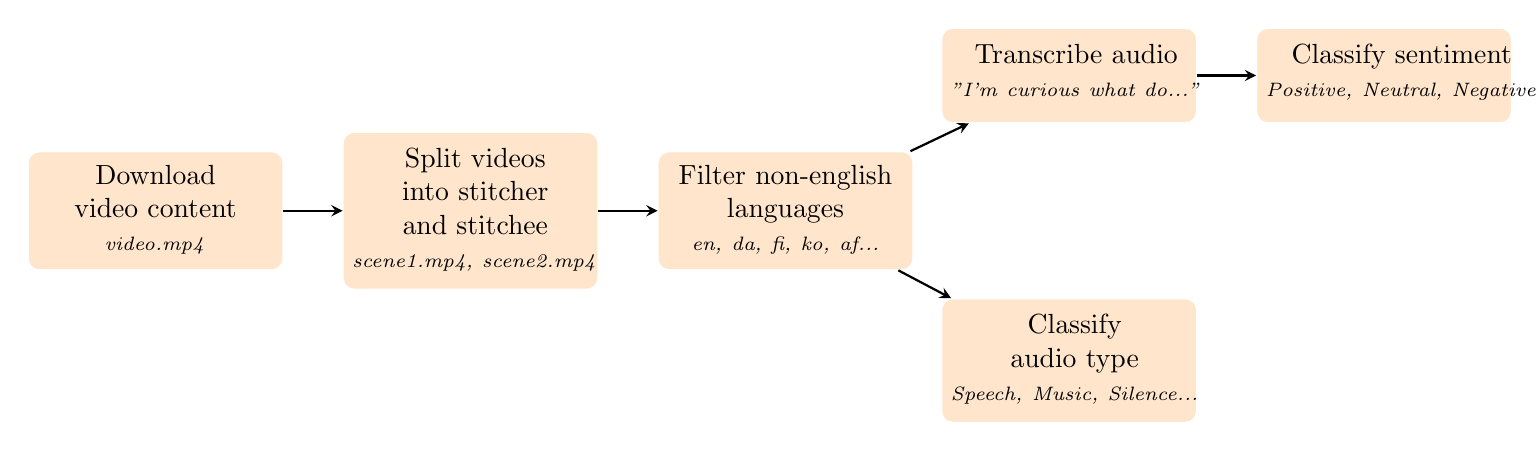
\begin{tikzpicture}[node distance=4cm]
    % Nodes
    \node (download)   [process] {\makecell{Download\\ video content\\ \scriptsize{\textit{video.mp4}}}};
    \node (split)      [process, right of=download] {\makecell{Split videos\\ into stitcher\\ and stitchee\\ \scriptsize{\textit{scene1.mp4, scene2.mp4}}}};
    \node (filter)     [process, right of=split] {\makecell{Filter non-english\\ languages\\ \scriptsize{\textit{en, da, fi, ko, af...}}}};
    \node (transcribe) [process, above right=0.5cm of filter] {\makecell{Transcribe audio\\ \scriptsize{\textit{"I'm curious what do..."}}}};
    \node (classify_aud) [process, below right=0.5cm of filter] {\makecell{Classify\\ audio type\\ \scriptsize{\textit{Speech, Music, Silence...}}}};
    \node (classify_sent)   [process, right of=transcribe] {\makecell{Classify sentiment\\ \scriptsize{\textit{Positive, Neutral, Negative}}}};
    
    % Arrows
    \draw [arrow] (download) -- (split);
    \draw [arrow] (split) -- (filter);
    \draw [arrow] (filter) -- (transcribe);
    \draw [arrow] (filter) -- (classify_aud);
    \draw [arrow] (transcribe) -- (classify_sent);
\end{tikzpicture}
 





% \begin{center}
% \begin{tikzpicture}[node distance=3.66cm]

% % \node (start) [startstop] {Start};
% % \node (process1) [process, right of=start] {Process 1};
% % \node (process2) [process, right of=process1] {Process 2};
% % \node (stop) [startstop, right of=process2] {Stop};

% % \draw [arrow] (start) -- (process1);
% % \draw [arrow] (process1) -- (process2);
% % \draw [arrow] (process2) -- (stop);

% % Nodes
% \node (download)   [process] {Download video content};
% \node (split)      [process, right of=download] {Split videos into stitcher and stitchee};
% \node (filter)     [process, right of=split] {Filter music and non-english languages};
% \node (transcribe) [process, right of=filter] {Transcribe audio};
% \node (classify)   [process, right of=transcribe] {Classify sentiment};

% % Arrows
% \draw [arrow] (download) -- (split);
% \draw [arrow] (split) -- (filter);
% \draw [arrow] (filter) -- (transcribe);
% \draw [arrow] (transcribe) -- (classify);


% \end{tikzpicture}
% \end{center}

% Download → Split → Filter → Transcribe → Sentiment labeling → Sentiment labeled graph

    \end{adjustwidth}
    \caption{The process by which videos are enriched with content data. Specifically, the video's spoken language, audio type, transcription, and sentiment are extracted.}
    \label{fig:dataaugmentation}
\end{figure}

\begin{comment}
%procenten af downloaded videoer vs edges som vi har
1232/1363=90%
137/145=94%
275/345=80%
463/555=83%
3329/3737=89%
550/600=92%
841/846=99%
44/46=96%
615/680=90%
431/480=90%
total=90%

(40653-227+86*2)/2

%total antal videoer
abortion: 45
\end{comment}

\textbf{Download video content:} 
The first step of the augmentation pipeline is downloading videos. Specifically, we download all available stitches and not the stitched videos. Neither TikTok's API nor the app supports downloading videos. Instead, we use \textit{Pyktok} \citep{Freelon_pyktok}, an unofficial Python library for collecting TikTok data. With this library, we download all available collected stitches, amounting to $86\%$, with the remaining $14\%$ not being available for download, either due to being removed or made private. This resulted in $20299$ total downloaded videos. 

\textbf{Split videos into stitcher and stitchee:}
The stitch videos that we obtain contain both the stitcher and stitchee parts in the same video. Since we aim to process the reactions to the stitched content, we separate the stitchers from the stitchees by splitting videos. To this end, we use the Python library \textit{scenedetect} \citep{PySceneDetect}, which detects scene changes by analyzing variations in the HSL (Hue, Saturation, Lightness) color space. Specifically, the adaptive detection method identifies abrupt cuts using a rolling average of color differences, and classifies a scene shift when the rolling average is above a set threshold. Using the adaptive detection method, we detect the scene shift that transitions from the stitchee part to the stitch part. 

%\setcounter{algorithm}{-1}
\begin{algorithm}
%\caption{Scene Detection for TikTok Videos (First 5 Seconds)}
\begin{algorithmic}[1]
\Require A stitch video
\Ensure The respective stitcher and stitchee parts of the video  %Split points for scene shifts or default at 5 seconds

\State $thresholds \gets [9, 6, 5]$ \Comment{Adaptive threshold for detecting scenes}
\State $splitPoint \gets 5$ \Comment{Default split point}
\State $videoSegment \gets \text{ExtractSegment}(\text{video}, 0, 5)$ \Comment{Only use the first 5s}

\For{$threshold$ in $thresholds$}
    \State $sceneShifts \gets \text{DetectSceneShifts}(videoSegment, threshold)$
    \If{$\text{length}(sceneShifts) > 0$}
%        \State $splitPoint \gets \text{LastDetectedShift}(sceneShifts)$
        \State $splitPoint \gets \text{GetLastSceneShift}(sceneShifts)$
        \State \textbf{break}
    \EndIf
\EndFor

\\
\State $\text{SplitVideoAt}(\text{video}, splitPoint)$ \Comment{Split video at detected split point}
\\

\Function{DetectSceneShifts}{$videoSegment$, $threshold$} \Comment{From \texttt{scenedetect}}
    \State \Return list of timestamps where scene shifts are detected based on $threshold$
\EndFunction
\end{algorithmic}
\caption{Pseudocode for splitting videos into stitcher and stitchee}
\label{pseudocode}
\end{algorithm}

The specific scene detection strategy, as described by Algorithm \ref{pseudocode}, is to detect all scene shifts that occur within the first five seconds with a set adaptive threshold. TikTok stitches can only include up to five seconds of the stitched content, which can be leveraged to focus scene shift detection exclusively on the first five seconds of stitches. If one or more scene shifts are detected, the videos are split at the last detected scene. If no scenes are detected, lower the adaptive threshold and repeat. This process is repeated for adaptive thresholds $9$, $6$, and $5$. If no scenes are detected with any of the thresholds, the videos are split at the five second mark, which also serves as a default split point in alignment with the five second limit for TikTok stitches. 



\textbf{Filter non-English languages:}
Many of the collected videos are in languages other than English. Since the applied sentiment analysis model is designed exclusively for English-language content, only videos in English are transcribed. To identify the language of each video, OpenAI's Whisper Model \citep{radford2022robustspeechrecognitionlargescale} is used, offering functionalities to classify the language of audio and video files, among other features.

\textbf{Classify audio type:}
TikTok videos often feature various audio types. Since our goal is to extract the sentiment of videos, it is essential to distinguish between speech and non-speech audio, such as music or other sounds. To achieve this, we apply Google's \textit{MediaPipe Audio Classifier} \citep{mediapipe_audio_classifier}, which classifies the audio type for each second of a video. This dimension provides insight into the dominant audio type within a video, which itself is useful for gaining a deeper understanding of the content, while also being useful for filtering transcriptions.

\textbf{Transcribe audio:}
To extract the textual component of each video, each English video is transcribed; both the stitch and the stitchee parts. Similarly to the \textit{Filter non-English languages} section, we also use the Whisper model but for transcriptions. The model has six sizes ranging from \textit{tiny} ($39$ million parameters) to \textit{turbo} ($809$ million parameters). As we do not possess expensive computing hardware, we opted to use the \textit{base} model ($74$ million parameters). A known limitation of Whisper is its $30$-second context window, which requires padding or pruning videos to this duration. An alternative approach would involve processing the audio input in batches. In our dataset, the proportion of videos shorter than $30$ seconds varies between hashtags. For example, $18$\% of the videos in the hashtag \textit{\#abortion} are shorter than $30$ seconds, while this percentage increases to $40$\% for \#football and $75$\% for both \textit{\#comedy} and \textit{\#dogsoftiktok}. In contrast, hashtags such as \textit{\#storytime} predominantly feature videos longer than $30$ seconds, reflecting a different narrative style. However, we assume that the $30$-second context limitation aligns well with TikTok's nature as a short-form video platform, where the general sentiment or core message of a video is often conveyed within the first $30$ seconds.

\textbf{Classify sentiment:}
To enrich the analysis of TikTok communication, we incorporate the sentiment analysis into the user graphs. While our focus is the communication structure, sentiment analysis provides additional insight while still allowing for comparison with Twitter, helping to explore whether platform differences influence communication dynamics. We use \textit{VADER Sentiment Analysis} (hereafter referred to as VADER) \citep{VADER} to analyze the transcribed text from stitcher videos, classifying the sentiment into positive, neutral, or negative categories. When videos are unavailable for download, or when no transcription exists, they are labeled with a separate 'no content' label. The result of the sentiment classification is sentiment augmented graphs, where video- and user graphs have assigned sentiments on the stitch relations, illustrated in Figure \ref{fig:biden_sentiment}. This enriched user graph enables frequent subgraph mining with sentiment-labeled edges, facilitating the identification of patterns tied to specific sentiment categories.


\begin{figure}[H]
    \centering
    \begin{subfigure}{0.5\textwidth}
        \centering
        \SetVertexStyle[Shape=circle, InnerSep=2, MinSize=14, FillColor=orange!40, LineColor=black, TextFont=\normalsize]
\SetEdgeStyle[Color=gray, Arrow=-stealth]

\begin{tikzpicture}
	\Vertex[x=-0.03, y=-0.88, label=$A$, color=VertexSentimentMissing]{0}
	\Vertex[x=-1.15, y=-1.17, label=$A$, color=VertexSentimentNeutral]{1}
	\Vertex[x=1.03, y=-1.01, label=$A$,  color=VertexSentimentPositive]{2}
	\Vertex[x=1.12, y=-2.15, label=$B$,  color=VertexSentimentMissing]{3}
	\Vertex[x=-0.74, y=1.70, label=$C$,  color=VertexSentimentPositive]{4}
	\Vertex[x=-1.72, y=1.51, label=$D$,  color=VertexSentimentNeutral]{5}
	\Vertex[x=-2.56, y=0.87, label=$C$,  color=VertexSentimentPositive]{6}
	\Vertex[x=-2.19, y=-0.18, label=$E$, color=VertexSentimentMissing]{7}
	\Vertex[x=-1.69, y=0.78, label=$F$,  color=VertexSentimentMissing]{8}
	\Vertex[x=-3.22, y=-0.72, label=$A$, color=VertexSentimentMissing]{9}
	\Vertex[x=-3.00, y=0.22, label=$F$,  color=VertexSentimentNeutral]{10}
	\Vertex[x=-2.44, y=-1.14, label=$G$, color=VertexSentimentNegative]{11}
	\Vertex[x=-1.88, y=-2.06, label=$F$, color=VertexSentimentNeutral]{12}
	\Vertex[x=-2.60, y=-2.44, label=$H$, color=VertexSentimentPositive]{13}
	\Vertex[x=-3.11, y=-1.59, label=$F$, color=VertexSentimentPositive]{14}
	\Vertex[x=-1.86, y=-2.95, label=$I$, color=VertexSentimentNeutral]{15}
	\Vertex[x=-0.82, y=-2.52, label=$J$, color=VertexSentimentNegative]{16}
	\Vertex[x=0.65, y=-2.79, label=$K$,  color=VertexSentimentNeutral]{17}
	\Vertex[x=0.06, y=-1.96, label=$L$,  color=VertexSentimentNegative]{18}
	\Vertex[x=-0.07, y=-3.11, label=$K$, color=VertexSentimentNegative]{19}
	\Vertex[x=-1.08, y=-3.25, label=$F$, color=VertexSentimentNegative]{20}
	\Vertex[x=-0.80, y=0.03, label=$K$,  color=VertexSentimentNeutral]{21}
	\Vertex[x=0.38, y=0.28, label=$F$,   color=VertexSentimentNeutral]{22}
	\Vertex[x=0.26, y=1.41, label=$K$,   color=VertexSentimentMissing]{23}
	\Vertex[x=0.93, y=0.98, label=$K$,   color=VertexSentimentMissing]{24}
	\Vertex[x=1.41, y=0.17, label=$D$,   color=VertexSentimentPositive]{25}
	\Vertex[x=-0.49, y=1.03, label=$I$,  color=VertexSentimentMissing]{26}
	\Vertex[x=1.59, y=-1.54, label=$I$,  color=VertexSentimentNegative]{27}
	\Vertex[x=1.65, y=-0.49, label=$M$,  color=VertexSentimentNegative]{28}
	\Edge[Direct](0)(1)
	\Edge[Direct](2)(3)
	\Edge[Direct](4)(5)
	\Edge[Direct](6)(5)
	\Edge[Direct](7)(8)
	\Edge[Direct](9)(10)
	\Edge[Direct](11)(12)
	\Edge[Direct](13)(14)
	\Edge[Direct](15)(16)
	\Edge[Direct](17)(18)
	\Edge[Direct](19)(20)
	\Edge[Direct](21)(22)
	\Edge[Direct](23)(22)
	\Edge[Direct](24)(25)
	\Edge[Direct](26)(22)
	\Edge[Direct](27)(28)
\end{tikzpicture}

        \caption{Sentiment video graph}
        \label{fig:biden_vgraph_sentiment}
    \end{subfigure}%
    \begin{subfigure}{0.5\textwidth}
        \centering
        \SetVertexStyle[Shape=circle, InnerSep=2, MinSize=14, FillColor=orange!40, LineColor=black, TextFont=\normalsize]
\SetEdgeStyle[Color=gray, Arrow=-stealth]

\begin{tikzpicture}
	\Vertex[x=-0.85, y=1.59, label=$A$]{0}
	\Vertex[x=-1.62, y=2.65, label=$B$]{1}
	\Vertex[x=3.00, y=-1.13, label=$C$]{2}
	\Vertex[x=2.1, y=-0.75, label=$D$]{3}
	\Vertex[x=0.40, y=1.67, label=$E$]{4}
	\Vertex[x=0.07, y=0.41, label=$F$]{5}
	\Vertex[x=-1.04, y=0.51, label=$G$]{6}
	\Vertex[x=1.34, y=0.97, label=$H$]{7}
	\Vertex[x=-0.9, y=-0.97, label=$I$]{8}
	\Vertex[x=-1, y=-2.12, label=$J$]{9}
	\Vertex[x=0.94, y=-0.52, label=$K$]{10}
	\Vertex[x=0.84, y=-1.66, label=$L$]{11}
	\Vertex[x=-2.11, y=-1.02, label=$M$]{12}
	\Edge[Direct, color=SentimentMissing](0)(0)
	\Edge[Direct, color=SentimentPositive](0)(1)
	\Edge[Direct, color=SentimentPositive, bend=-33](2)(3)
	\Edge[Direct, color=SentimentPositive, bend=33](2)(3)
	\Edge[Direct, color=SentimentMissing](4)(5)
	\Edge[Direct, color=SentimentMissing](0)(5)
	\Edge[Direct, color=SentimentNegative](6)(5)
	\Edge[Direct, color=SentimentPositive](7)(5)
	\Edge[Direct, color=SentimentNeutral](8)(9)
	\Edge[Direct, color=SentimentNeutral](10)(11)
	\Edge[Direct, color=SentimentNegative](10)(5)
	\Edge[Direct, color=SentimentNeutral, bend=-33](10)(5)
	\Edge[Direct, color=SentimentMissing, bend=33](10)(5)
	\Edge[Direct, color=SentimentMissing](10)(3)
	\Edge[Direct, color=SentimentMissing](8)(5)
	\Edge[Direct, color=SentimentNegative](8)(12)
\end{tikzpicture}

        \caption{Sentiment user graph}
        \label{fig:biden_ugraph_sentiment}
    \end{subfigure}
    \caption{Example user- and video graph, created from a sample of \textit{\#biden2024}, augmented with sentiment. Possible sentiment labels are \textcolor{SentimentPositive}{positive}, \textcolor{SentimentNeutral}{neutral}, \textcolor{SentimentNegative}{negative}, and \textcolor{SentimentMissing}{no content}. In the video graph, each video (vertex) is assigned the sentiment of the video transcription. Transitioning to the user graph, each video (edge) is assigned the sentiment of the stitcher's transcription. Thus, it models user's reactions towards other user's content. This figure is an extension of Figure \ref{fig:biden}.}
    \label{fig:biden_sentiment}
\end{figure}



% On TikTok creators often want their videos to reach many people, and thus optimize for the algorithm. The Tiktok algorithm is not public, but people have found that it heavily punishes bad words, and thus creators have found their way around by using "Algospeak", which is a way of changing the word you want to say by some non-offensive word, e.g. "kill" to "unalive" \citep{doi:10.1177/20563051231194586}. As we expect this could affect our sentiment analysis, we do a quick check of how often algospeak is used in our data, and how it affects the sentiment. We find that "I wanna unalive you" has a completely neutral compound score of 0.0 vs "I wanna kill you", which has a compound score of –0.69 (very negative). "I hate you" is -0.57 (very negative) and "I opposite of love you" is almost the exact opposite at 0.63 (very positive). So it can have a big impact on the sentiment we get, even with these very simple examples. More complex ones include can even include body language instead of saying the word. Our transcription can only detect some of these, which fortunately don't occur too often, e.g. "unalive" is in our dataset 14 times, so we decide to not account for algospeak in the sentiment analysis.



\section{Twitter: A Comparative Perspective}\label{twitter_data_and_material}

Twitter serves as an important point of comparison in this study. Unlike TikTok’s video-based, multimodal content, Twitter’s reply networks are focused on text-based interactions, where users respond directly to tweets and other replies. For this paper, we use existing Twitter data, provided by \cite{doi:10.1126/sciadv.abq2044}, and presented in Table \ref{tab:twitter_table}. This data, from which we construct the reply networks, centers around six topics and events: gun control, pro-choice, abortion, a vice presidential debate, a second presidential debate, and the U.S. Supreme Court ruling on Obamacare. This is fundamentally different from our StitchGraph dataset, which consists of all stitches from specific hashtags, while the Twitter dataset is a collection of tweets containing at least one of a couple keywords per overall topic. The datasets are composed by \cite{doi:10.1126/sciadv.abq2044} but originate from a collection of previous research. Due to the differing data sources, the specific data collection details vary between networks, and as such, it is important to be mindful of the diverse data collection practices when using the data. The dataset reflects a snapshot of political discourse from around a decade ago. Since then, the political landscape surrounding key issues such as abortion and gun control has evolved significantly, influenced by changes in public opinion, policy changes, and new social movements. This gap highlights the need to be aware of changes over time, as the discussions around these topics today may diverge significantly from then.

\begin{table}[h]
    \centering
    \begin{adjustwidth}{-\textwidth}{-\textwidth}
        \centering
        \begin{tabular}{l|rrrrr|rrrrrrrr}
    \toprule
    \multicolumn{1}{c|}{} & \multicolumn{5}{c|}{Full graph} & \multicolumn{7}{c}{Largest weakly connected component} \\ 
               Topic &  $|V|$ &  $|E|$ & \makecell{\#Compo-\\nents} & $D$ &  $D_u$ &  $|V|$ &  $|E|$ &  $L$ &  $L_u$ &  $C_u$ &  Reciprocity &  \makecell{Degree\\ centralization} \\ 
    \midrule
        Second debate &   1556 &   3248 &                        163 &   2 &     14 &    986 &   2584 & 1.00 &   5.01 &   0.00 &         0.00 &                                0.20 \\
      Election &   1381 &   2266 &                        367 &   1 &     14 &    734 &   1296 & 1.00 &   5.29 &   0.00 &         0.00 &                                0.08 \\
            VP debate &   1330 &   2756 &                        158 &   2 &     12 &    932 &   2325 & 1.00 &   4.80 &   0.00 &         0.00 &                                0.18 \\
      Abortion &   1081 &   1277 &                        186 &   6 &     18 &    690 &    946 & 1.91 &   7.09 &   0.00 &         0.01 &                                0.10 \\
    Guncontrol &    284 &    239 &                        116 &   2 &      6 &     11 &     11 & 1.23 &   3.05 &   0.00 &         0.00 &                                0.14 \\
         Obamacare &     74 &    108 &                         27 &   1 &      4 &     12 &     11 & 1.00 &   1.83 &   0.00 &         0.00 &                                1.00 \\
    \bottomrule
\end{tabular}
    \end{adjustwidth}
    \caption{Selected metrics for the Twitter reply networks for both the full graphs and their largest weakly connected components. These are comparable with the TikTok user graphs, with edges mapping interactions (replies) between users.}
    \label{tab:twitter_table}
\end{table}

\begin{comment}
    
In the following paragraphs, we outline the most significant details of the data composition. 

\textbf{Election}:
This dataset, sourced from \cite{kerchner2020coronavirus}, includes 51,425 tweets. Tweets were filtered to include only those linking to URLs on \href{https://www.mediabiasfactcheck.com/}{www.mediabiasfactcheck.com}. 
Users who tweeted less than three times were excluded to maintain consistency.

\textbf{Gun Control, Obamacare, and Abortion Networks}:
Based on \cite{garimella2018political}, this dataset focuses on three major events:
\begin{itemize}
    \item \textbf{Gun Control:} Democrat filibuster for gun control reforms (June 12–18, 2016), containing 7,811 tweets.
    \item \textbf{Obamacare:} Supreme Court ruling on subsidies (June 22–29, 2015), with 970 tweets.
    \item \textbf{Abortion:} Supreme Court strikes down Texas abortion restrictions (June 27–July 3, 2016), with 36,045 tweets. 
\end{itemize}
These tweets were collected within a 3-day window before and after each event and filtered using specific keywords from \cite{lu2015biaswatch}. 

Finally, we obtained two networks related to the \textbf{presidential debates} of 2012: one from the second presidential debate, consisting of $37,849$ tweets, and another from the vice presidential debate, containing $32,194$ tweets.
\end{comment}

The Twitter reply networks are multi-digraphs, where vertices are users that have tweeted tweets that conform to the data collection criteria, and edges are replies directed from the replying user to the source user. This is similar to the TikTok user graphs, where the vertices are users, and edges are the stitch relations between them. Although Twitter allows for replying to a reply, unlike stitches on TikTok, there is still very little reciprocity. %In general, we consider the metrics and methods for data gathering similar enough to allow for meaningful comparison.

To also compare sentiment findings, we apply VADER to analyze the sentiment of tweets, obtaining a sentiment score for each one. In contrast to TikTok, Twitter is a text-dominated platform, and all tweets contain a textual component, meaning that sentiment analysis can be performed on all tweets. 

% The vertices in the various Twitter networks are Tweets that conforms with the previously mentioned criteria. The edges are interactions between two users, where \textit{User\_a} replies to \textit{User_b} one or more times. This   

% Twitter does allow for replying to a reply, as opposed to TikTok, but as seen in Table \ref{tab:twitter_table}, there is still very little reciprocity. In general we consider the metrics and method for data gathering similar enough for comparison.



% Twitter serves as an important point of comparison for this study. Unlike TikTok's multimodal content, Twitter’s reply network provides a structured, text-dominated interaction system in which users respond directly to other posts. This allows us to examine how platform affordances and content formats might shape communication networks.
% For this comparison, we use Twitter data from 2013, focusing on reply networks constructed around six topics/events: \textit{gun-control}, \textit{pro-choice}, \textit{abortion}, \textit{vicepresidential debate}, \textit{second presidential debate}, and \textit{Obamacare U.S. supreme court ruling} \citep{doi:10.1126/sciadv.abq2044}. To guarantee a fair comparison, the same hashtag data are extracted from TikTok as well, providing a common thematic ground for cross-platform analysis. By applying the same methodologies, namely, graph embeddings, frequent subgraph mining, and network property analyzes, we aim to explore differences and similarities in the communication structures of the two platforms. While we expect structural differences given the platforms' distinct affordances (e.g., video versus text), our use of analytical methods enables us to identify whether content type or platform design plays a larger role in shaping network structures. For instance, we are interested in determining whether highly polarized topics such as those examined here produce similar motifs or clustering behaviors on TikTok and Twitter.




% -------------------------------------------------------------------

\begin{comment}
    
The first step in our analysis is choosing the right hashtags to study. We aim to select hashtags that provide useful insights while ensuring the data we collect is neither too large nor too small. We avoid hashtags that are too big, as they would make the network too complex to analyze, and we also stay away from very small hashtags that do not have enough stitching activity to be meaningful. Instead, we focus on hashtags that represent specific communities or interests, rather than general tags like \textit{\#trending} or \textit{\#foryou}.

We also select hashtags where English is the main language. Moreover, it is important that the hashtags were used in May 2024, which is when we collect our data. This is due to the TikTok Research API not working as expected when it is prompted for too much data. But at the same time we want data for long enough that we can expect to get most of the full conversations. Also it cannot be too recent, as the API doesn't include everything immediately. Include info on how far back in time people stitch, to support this.
Another factor we consider is whether the hashtags are likely to include videos with conversations or interactions, as this is key to studying how users respond to each other through stitching.

To find these hashtags, we look at popular TikTok tags\footnote{https://tiktokhashtags.com/best-hashtags.php} and those mentioned in academic studies related to our project. We group the hashtags into three categories: \textbf{shared interest/subculture}, "\textbf{political discussion}", and "\textbf{entertainment/knowledge}, because we expect each group to have its own style of communication. For instance, hashtags in the shared interest category are likely used by more close-knit communities, while the entertainment hashtags probably attract a wider audience with less specific interests. Although political hashtags cover different topics, we expect them to show similar patterns in how people interact compared to the other groups. This process helps us choose a variety of hashtags that provide a solid foundation for our analysis.




\begin{verbatim}
{
  "7375311790760086827": {
    "hashtag_names": [
      "anime",
      "stitch",
      "onepiece",
      "fyp",
      "big3",
      "debate",
      "greenscreen"
    ],
    "id": 7375311790760086827,
    "is_stem_verified": false,
    "region_code": "US",
    "username": "nojcoeur",
    "video_description": "#stitch with @OXGhosty \u304e \u309c
    #greenscreen What anime should be the \u201cBIG 5\u201d?
    #anime #big3 #onepiece #fyp #debate ",
    "view_count": 91,
    "create_time": 1717198596,
    "is_stitcher": true,
    "stitches": 7236855455346134315,
    "is_stitchee": false
  }
}
\end{verbatim}


\section{Data Description}
Some calls to the API doesn't give responses, TikTok states that there are some filters, of which examples are for users under 18 and users in Canada. Videos can also have been deleted, by the user or by TikTok, or made private by the user. These can be very different things, but both are assumed in this project, to not happen too often, for it to significantly change the results.

For each video we can get a number of fields, of which we chose to gather the following:
\begin{itemize}
    \item id: unique identifier
    \item is\_stem\_verified: true/false if TikTok decided to include it in the STEM feed
    \item region\_code: the region the user registered in
    \item username: the video's author's username
    \item video\_description: description/title of video, if stitch as standard it starts with "\#stitch with @\textit{stitchee}
    \item view\_count: number of times the video has been seen for at least 1 second, 3 seconds for long videos
    \item create\_time: UTC Unix epoch (in seconds) of when the video was posted
    \item is\_stitcher: true/false if this video is stitching another video
    \item stitches: id of the stitched video
    \item is\_stitchee: true/false if this video is stitched
\end{itemize}



\section{Exploratory Data Analysis}
We compute basic network metrics for both the video graph and user graph for all the hashtags, as well as the degree assortativity, and centralization in terms of degree, betweenness, and closeness, which we compute for both the full hashtag network, and for the largest connected component of the user graphs. In the user graphs, the number of vertices range from x-y, and the number of edges range from x-y, with largest connected component ranging from x-y and number of components ranging from x-y. There is no reciprocity in any of the networks.
Table \ref{Video Metrics} shows these metrics for the video graph, and Table \ref{User Metrics} for the user graph. As a stitch cannot be stitched, some of these metrics are the same in the video graph.


% \textbf{TO INCLUDE:}
% \begin{itemize}
%     \item \textbf{Data Collection}:
%     \begin{itemize}
%         \item Sources: Where did the data come from? (e.g., databases, surveys, APIs)
%         \item Process: How was the data collected? (e.g., automated scraping, manual entry)
%         \item Tools/Technologies: Tools or technologies used for collection (e.g., Python scripts, SQL queries)
%     \end{itemize}
    
%     \item \textbf{Data Description}:
%     \begin{itemize}
%         \item Characteristics: What does the dataset look like? (e.g., size, features, types of data)
%         \item Sample Data: Provide a snapshot or example of the data.
%     \end{itemize}

%     \item \textbf{Exploratory Data Analysis (EDA)}:
%     \begin{itemize}
%         \item Descriptive Statistics: Summarize the main characteristics of the data (e.g., mean, median, standard deviation)
%         \item Visualizations
%         \item Patterns/Trends: Any noticeable patterns, trends, or anomalies in the data.
%     \end{itemize}

%     \item \textbf{Data Quality Issues}:
%     \begin{itemize}
%         \item Missing Data: How much missing data is there, and how was it handled?
%         \item Errors: Any errors or inconsistencies found in the data and how they were addressed.
%         \item Biases: Potential biases in the data collection process.
%     \end{itemize}

%     \item \textbf{Preprocessing}:
%     \begin{itemize}
%         \item Cleaning: Steps taken to clean the data (e.g., removing duplicates, handling missing values)
%         \item Transformation: Any transformations or feature engineering done (e.g., normalization, encoding)
%     \end{itemize}

%     \item \textbf{Data Analysis/Modeling}:
%     \begin{itemize}
%         \item Techniques: Methods and algorithms used for analysis (e.g., regression, clustering, classification)
%         \item Evaluation: How the results were evaluated (e.g., metrics, cross-validation)
%     \end{itemize}

%     \item \textbf{Challenges and Limitations}:
%     \begin{itemize}
%         \item Technical Challenges: Any technical issues faced during data collection or analysis.
%         \item Limitations: Limitations of the dataset and how they might affect the results.
%     \end{itemize}

%     \item \textbf{Ethics} (if applicable):
%     \begin{itemize}
%         \item Data Privacy: Considerations related to data privacy and consent.
%     \end{itemize}
% \end{itemize}




\end{comment}

\label{datagathering}



\chapter{Method}
% This paper examines the structural patterns of TikTok stitch networks to quantitatively compare the topologies of different graphs and hashtag categories in TikTok StitchGraph. By analyzing whether hashtags within the same category exhibit structural similarity, the goal is to uncover patterns in how users interact and communicate on the platform. Two main approaches are employed: subgraph analysis and graph embeddings. Subgraph analysis identifies recurring subgraphs that compose the observed communication patterns within stitch networks, while graph embeddings project the networks into a lower-dimensional space to assess similarities and differences between hashtag groups. By combining subgraph analysis with graph embeddings, both micro-level patterns (e.g., motifs like star structures or chains) and macro-level patterns (e.g., clustering of hashtag categories) are detected. This dual approach facilitates a more comprehensive understanding of the communication dynamics on TikTok.

This paper examines the structural patterns of TikTok stitch networks to quantitatively compare the topologies of different graphs and hashtag categories in TikTok StitchGraph. By analyzing whether hashtags within the same category exhibit structural similarity, the goal is to uncover patterns in how users interact and communicate on the platform. Two main approaches are employed: subgraph analysis and graph representation learning. Subgraph analysis identifies recurring subgraphs that form the observed communication patterns within stitch networks, while graph representation learning focuses on deriving graph-level embeddings to represent the networks in a lower-dimensional space, enabling the evaluation of similarities and differences between hashtag groups within the learned vector representation. By combining subgraph analysis with graph embeddings, both micro-level patterns (e.g., motifs like star structures or chains) and macro-level patterns (e.g., clustering of hashtag categories) are detected. This dual approach facilitates a more comprehensive understanding of the communication dynamics on TikTok.


The presented methodology is only applied to user graphs, and not video graphs. The focus is on user graphs because they capture broader interaction patterns between users, and because of the platform-enforced constraints on video graphs. Analysis of user graphs reveals insights into user stitch behavior. Furthermore, the results of the methods are compared with Twitter reply networks to offer context and perspective from a similar well-studied social network.

% With the collected dataset, we aim to explore the structure of communication of stitches on TikTok using various network approaches. The goal is to ... We work on usergraphs... Both for standard graph and for sentiment graphs...

% Something something software used. Python 3.x, iGraph, Karate Club, networkx...


\section{Frequent Subgraph Mining}
To identify characteristic stitch patterns on TikTok, the \textit{subgraphs} that constitute the observed TikTok stitch user graphs are examined. The objective is to identify the \textit{motifs} that characterize communicative patterns on TikTok. To this end, \textit{frequent subgraph mining} is employed, a technique used to discover subgraphs that appear repeatedly within a graph \citep{coscia2021atlasaspiringnetworkscientist}. Specifically, \textit{transactional graph mining} is applied, aiming to identify subgraphs that frequently occur across a collection of graphs. In practice, this involves pruning the subgraph search space by constraining the minimum required \textit{support} of a subgraph. In a transactional setting, the support of a subgraph is the number of graphs in the graph set with which the subgraph is \textit{isomorphic}, as illustrated in Figure \ref{fig:fsm}. Note that this is fundamentally different from \textit{single graph mining}, where support is defined as the number of isomorphisms between a subgraph and a single graph. An important implication of the transactional setting is that the mined subgraphs may vary in how representative they are of specific graphs. Under the transactional support definition, a subgraph is treated as equally representative of all graphs in which it appears, even if its frequency within the graphs differs.

\begin{figure}[h]
    \centering
    % style
\SetVertexStyle[Shape=circle, InnerSep=1, MinSize=5, FillColor=black!75, LineColor=black!75]
\SetEdgeStyle[Color=gray, Arrow=-stealth]
\definecolor{ForestGreen}{rgb}{0.13, 0.55, 0.13}

% motifs
% \newcommand{\MotifOne}{
% \begin{tikzpicture}
%     \Vertex[x=-0.66, y=0.00]{0}
%     \Vertex[x=0.00, y=0.00]{1}
%     \Vertex[x=0.66, y=0.00]{2}
%     \Edge[Direct, color=SentimentPositive](0)(1)
%     \Edge[Direct, color=SentimentNegative](2)(1)
% \end{tikzpicture}
% }

\newcommand{\MotifOne}{
\begin{tikzpicture}
    \Vertex[x=0.33, y=0.33]{0}
    \Vertex[x=-0.33, y=0.00]{1}
    \Vertex[x=0.33, y=-0.33]{2}
    \Edge[Direct, color=SentimentPositive](0)(1)
    \Edge[Direct, color=SentimentNegative](2)(1)
\end{tikzpicture}
}

% \newcommand{\MotifTwo}{
% \begin{tikzpicture}
%     \Vertex[x=-0. 66, y=0.00]{0}
%     \Vertex[x=0.00, y=0.00]{1}
%     \Vertex[x=0.66, y=0.00]{2}
%     \Edge[Direct, color=SentimentPositive](0)(1)
%     \Edge[Direct, color=SentimentNeutral](1)(2)
% \end{tikzpicture}
% }

\newcommand{\MotifTwo}{
\begin{tikzpicture}
    \Vertex[x=0.33, y=0.33]{0}
    \Vertex[x=-0.33, y=0.00]{1}
    \Vertex[x=0.33, y=-0.33]{2}
    \Edge[Direct, color=SentimentPositive](0)(1)
    \Edge[Direct, color=SentimentNeutral](1)(2)
\end{tikzpicture}
}

\newcommand{\MotifThree}{
\begin{tikzpicture}
    \Vertex[x=0.33, y=0.33]{0}
    \Vertex[x=-0.33, y=-0.33]{1}
    \Edge[Direct, bend=-33, color=SentimentPositive](0)(1)
    \Edge[Direct, bend=33, color=SentimentNegative](0)(1)
\end{tikzpicture}
}

\newcommand{\MotifFour}{
\begin{tikzpicture}
    \Vertex[x=0.33, y=0.33]{0}
    \Vertex[x=0, y=0]{1}
    \Vertex[x=0.33, y=-0.33]{2}
	\Vertex[x=-0.33, y=-0.33]{3}
	\Edge[color=SentimentPositive,Direct](0)(1)
	\Edge[color=SentimentPositive,Direct](2)(1)
	\Edge[color=SentimentPositive,Direct](3)(1)
\end{tikzpicture}
}

% graphs
\newcommand{\GraphOne}{
\begin{tikzpicture}
	\Vertex[x=0.75, y=-0.66]{0}
	\Vertex[x=0.33, y=0]{1}
	\Vertex[x=-0.33, y=0]{2}
	\Vertex[x=-0.75, y=-0.66]{3}
	\Vertex[x=0.75, y=0.66]{4}
	\Vertex[x=-0.75, y=0.66]{5}
	\Edge[color=SentimentPositive,Direct](0)(1)
	\Edge[color=SentimentNegative,bend=-33,Direct](2)(1)
	\Edge[color=SentimentPositive,bend=33,Direct](2)(1)
	\Edge[color=SentimentNeutral,Direct](2)(3)
	\Edge[color=SentimentPositive,Direct](4)(1)
	\Edge[color=SentimentNeutral,Direct](2)(5)
\end{tikzpicture}
}

\newcommand{\GraphTwo}{
\begin{tikzpicture}
	\Vertex[x=0, y=0.75]{0}
	\Vertex[x=0, y=0]{1}
	\Vertex[x=0.4, y=-0.66]{2}
	\Vertex[x=-0.4, y=-0.66]{3}
	\Vertex[x=0.75, y=0.2]{4}
	\Vertex[x=-0.75, y=0.2]{5}
	\Edge[color=SentimentPositive,Direct](0)(1)
	\Edge[color=SentimentNeutral,Direct](2)(1)
	\Edge[color=SentimentPositive,Direct](3)(1)
	\Edge[color=SentimentNeutral,Direct](4)(1)
	\Edge[color=SentimentPositive,bend=-33,Direct](5)(1)
	\Edge[color=SentimentPositive,bend=33,Direct](5)(1)
\end{tikzpicture}
}

%\newcommand{\GraphThree}{
%\begin{tikzpicture}
%	\Vertex[x=0, y=0]{0}
%	\Vertex[x=0.5, y=0]{1}
%	\Vertex[x=0, y=0.5]{2}
%	\Vertex[x=0, y=-0.5]{3}
%	\Vertex[x=0, y=-1.0]{4}
%    \Vertex[x=-0.5, y=0]{5}
%    \Vertex[x=0, y=0.525, opacity=0, size=0]{6}
%	\Edge[color=SentimentNeutral,Direct](0)(1)
%	\Edge[color=SentimentPositive,Direct](2)(0)
%	\Edge[color=SentimentPositive,Direct](0)(3)
%	\Edge[color=SentimentNegative,Direct](4)(3)
%    \Edge[color=SentimentNeutral,Direct](0)(5)
%\end{tikzpicture}
%}
\newcommand{\GraphThree}{
\begin{tikzpicture}
	\Vertex[x=0, y=0]{0}
	\Vertex[x=0, y=0.5]{1}
	\Vertex[x=-0.5, y=0]{2}
	\Vertex[x=0.5, y=0]{3}
	\Vertex[x=1, y=0]{4}
    \Vertex[x=0, y=-0.5]{5}
	\Edge[color=SentimentNeutral,Direct](0)(1)
	\Edge[color=SentimentPositive,Direct](2)(0)
	\Edge[color=SentimentPositive,Direct](0)(3)
	\Edge[color=SentimentNegative,Direct](4)(3)
    \Edge[color=SentimentNeutral,Direct](0)(5)
\end{tikzpicture}
}




% \begin{tabular}{cccccc}
%     & Subgraph & \multicolumn{3}{c}{Graph set} & Support \\
%     &  & \GraphOne & \GraphTwo & \GraphThree &  \\
%     \multirow{4}{*}{} & \MotifOne & X & & X & 2 \\
%     & \MotifTwo & & & X & 1 \\
%     & \MotifThree & X & & & 1 \\
%     & \MotifFour & X & X & & 2 \\
% \end{tabular}


\setlength\extrarowheight{20pt}
\begin{tabular}{c | c | c | c | c}
     \multicolumn{5}{c}{\raisebox{.3em}{Graph set}} \\ 
    % & & & & &  \\[-5.9em]
    \raisebox{.3em}{Subgraph} & \GraphOne & \GraphTwo & \raisebox{0.47em}{\GraphThree} & \raisebox{.3em}{Support} \\ \hline
    \MotifOne & \raisebox{.8em}{\textcolor{ForestGreen}{\faCheck}} & \raisebox{.8em}{\textcolor{red}{\faTimes}} & \raisebox{.8em}{\textcolor{ForestGreen}{\faCheck}} & \raisebox{.8em}{2} \\ \hline
    \MotifTwo & \raisebox{.8em}{\textcolor{red}{\faTimes}} & \raisebox{.8em}{\textcolor{red}{\faTimes}} & \raisebox{.8em}{\textcolor{ForestGreen}{\faCheck}} & \raisebox{.8em}{1} \\ \hline
    \MotifThree & \raisebox{.8em}{\textcolor{ForestGreen}{\faCheck}} & \raisebox{.8em}{\textcolor{red}{\faTimes}} & \raisebox{.8em}{\textcolor{red}{\faTimes}} & \raisebox{.8em}{1} \\ \hline
    \MotifFour & \raisebox{.8em}{\textcolor{ForestGreen}{\faCheck}} & \raisebox{.8em}{\textcolor{ForestGreen}{\faCheck}} & \raisebox{.8em}{\textcolor{red}{\faTimes}} & \raisebox{.8em}{2}
\end{tabular}




    \caption{The figure illustrates transactional frequent subgraph mining. Four example subgraphs are compared against the graph set to determine whether each subgraph is isomorphic to any induced subgraph from the graph set. The support of a subgraph is defined as the number of graphs in the set, where the subgraph appears. A checkmark \textcolor{ForestGreen}{\faCheck} indicates that the subgraph is found in a graph, while a cross \textcolor{red}{\faTimes} indicates it is not.}
    \label{fig:fsm}
\end{figure}

The need for isomorphism checks makes the process of frequent subgraph mining computationally intensive. Isomorphism itself is an NP-intermediate problem \citep{aaronson2016p}, and mining frequent subgraphs requires frequent isomorphism checks. This makes it difficult to implement frequent subgraph mining ourselves, and instead we opt for existing implementations, namely \textit{gSpan} \citep{yan2002gspan} and \textit{MoSS} \citep{borgelt2002moss}. We use these to mine undirected and directed structures, respectively. 

In this study, subgraphs are mined from both standard user graphs and sentiment-augmented user graphs. This approach enables us to analyze the purely topological structure of stitch communication, as well as the influence of sentiment on these topological patterns. This is done by assigning an \textit{edge color} (edge attribute) to each edge based on the sentiment of the stitch. Specifically, stitchees are assigned sentiment as an edge color since the goal is to find patterns in the reactions. We create four classes of sentiment; a positive, neutral, negative, and missing content class. 


We conduct all frequent subgraph mining on both the complete TikTok user graphs and their largest weakly connected components. All mined subgraphs are subsequently compared with Twitter graphs and relevant configuration models to compute their support for these. For this reason, we use iGraph's isomorphism function (\texttt{subisomorphic\_vf2}) for computing the support in subgraphs after they are mined\footnote{Note, in our experiments, we occasionally observed a slight difference between iGraph's computed support and the mined support from gSpan or MoSS. In this paper, we always report iGraph's computed support unless stated otherwise.} to have a comparable support between TikTok, Twitter, and configuration models. In conjunction with mining both undirected and directed graphs, we mine both purely structural patterns and sentiment patterns, resulting in eight separate frequent subgraph mining runs. 

When mining subgraphs, all self-loops are removed, but due to computational constraints, multi-edges are removed in the non-sentiment graphs. Although gSpan cannot find multigraph subgraphs, it can find simple subgraphs from a multigraph. MoSS can find multi-graph subgraphs, but it does not support self-loops. When computing the support of each mined subgraph, all self-loops and multi-edges are removed from the graph set, as their presence hinders isomorphism checks in iGraph\footnote{As of \texttt{iGraph 0.11.6}, \texttt{subisomorphic\_vf2} does not support self-loops. Furthermore, despite no documentation stating missing support for multi-edges, we empirically found that two non-isomorphic graphs can falsely return as isomorphic by iGraph if the subgraph contains a multi-edge.}. 

% Additionally, gSpan does not support multi-edges, and, based on our experience, MoSS could not complete successfully with multi-edges in the non-sentiment graphs, so these were removed. The only exception is directed sentiment graphs, with which we retain multi-edges during the mining process. 

\subsection{Undirected Subgraph Mining with gSpan}
To mine undirected subgraphs, we use gSpan \citep{yan2002gspan}. gSpan uses a minimum DFS code technique to build a lexicographic order of graphs and then subsequently uses a depth first search strategy to mine frequent connected subgraphs. For this study, we use a \texttt{C++} implementation of gSpan, provided by \cite{yan2009gspansoftware}, and ran the experiments in a \texttt{Pop!-OS} environment. To do this, all graphs are converted into a \texttt{.gspan} file format, and provided to the algorithm. gSpan supports mining from graphs with multi-edges, but does not support finding multi-edge subgraphs. We mine subgraphs down to a support threshold of $60\%$ without constraints on subgraph size. 

\subsection{Directed Subgraph Mining with MoSS}
To mine directed subgraphs, we use Molecular Substructure Miner (MoSS) \citep{borgelt2002moss}. MoSS is another frequent subgraph mining algorithm, originally developed for mining subgraphs in molecules. We use it to mine directed frequent subgraphs, as gSpan does not support edge direction. Specifically, we use a special implementation from \cite{gamer_moss}, implemented in \texttt{Java}, that supports general-purpose directed subgraph mining. MoSS employs a depth first search strategy to explore the search tree of possible subgraphs in a strategy similar to Eclat \citep{zaki1997new}, and prunes the search tree using support-based, size-based, and structural-based pruning. Pruning limits the search space based on the minimum support threshold, the maximum subgraph size limit, and ensures that each subgraph appears only in one branch of the search tree. In mining TikTok graphs, we prune the search tree by limiting the maximum substructure size to $|V|=4$ as the search tree grew too large for larger substructures and resulted in memory issues. MoSS does not support self-loops, but has no other topological restrictions. Using edge attributes in the form of sentiment classes prunes the search tree enough allowing for multi-edge mining, whereas with the unattributed version, we ran into computational constraints, leading us to mine simple no-sentiment substructures. 

\subsection{Discovering Motifs}\label{nullmodel_intro}
While the discovered subgraphs provide insight into the common patterns in the different graphs, this does not mean that these are significant. These subgraphs could appear in any graph of similar size. If a subgraph is significant, it is referred to as a motif. To discover motifs, the subgraphs should be compared to a relevant null model \citep{coscia2021atlasaspiringnetworkscientist}. A common choice for a null model is the configuration model, which preserves the degree distribution of the original graph while randomizing their connections. Comparison to this null model reveals whether the candidate motifs are significant or a product of the degree distribution. To account for randomness in the configuration models, $10$ configuration models are instantiated for each user graph. Comparisons to configuration models are only conducted for non-attributed graphs, meaning we do not do this for sentiment graphs. 

%For further comparison, we also compare this with an Erdös-Rényi random graph. 


\section{Graph Embeddings}
Graph embeddings provide a powerful framework to represent relationships and interactions in complex systems. By simplifying high-dimensional and intricate network structures, they map these systems into a lower-dimensional vector space, with the goal of capturing their structural and topological properties in numerical form.

In this study, graph embeddings are applied to analyze the structure of user graphs. Specifically, we embed and cluster $36$ distinct graphs, each representing a specific hashtag. These hashtags are divided into three predefined groups based on their themes (see Section \ref{hashtag_groups}). By studying embeddings and their clusters, we evaluate whether hashtags within a specific theme share structural properties distinct from those in other groups, offering insight into how stitch patterns vary between content topics.

\subsection{Graph Representation Learning with Graph2Vec}
To encode the graphs, we use \textit{Graph2Vec} \citep{graph2vec}, implemented by the Karate Club library \citep{karateclub}. As a method for graph representation learning, Graph2Vec encodes entire graphs into fixed-length embeddings, preserving both structural and topological characteristics. Inspired by \textit{Word2Vec} \citep{word2vec} and \textit{Doc2Vec} \citep{doc2vec}, Graph2Vec represents individual graphs as "documents" and rooted subgraphs as "words." Using the Weisfeiler-Lehman relabeling strategy \citep{shervashidze2011weisfeiler}, it captures both local and global features of the graphs. Graph2Vec adapts Doc2Vec’s skip-gram model, where the context window corresponds to the neighborhood captured by the Weisfeiler-Lehman relabeling. This skip-gram approach helps learn vector representations, which can be applied to tasks such as clustering and classification. However, like many neural representation learning methods, Graph2Vec is somewhat opaque: while we can observe the final embeddings and evaluate them in downstream tasks, it is difficult to pinpoint which specific graph structures map to particular dimensions of the resulting vectors, making it a black box algorithm. Due to the limitations of the Karate Club Library, we only apply Graph2Vec on simple graphs, i.e. we prune self-loops and multi-edges from the graphs. Lastly, Graph2Vec does not support edge-attributed graphs, and hence we refrain from embedding the sentiment graph with Graph2Vec. 

\subsection{Bag-Of-Subgraphs - A subgraph-based Graph Representation}
To represent entire graphs, a Bag-Of-Subgraphs approach is employed. The mined subgraphs from frequent subgraph mining can be used to define a subgraph-graph occurrence matrix to extract vector representations for entire graphs. This approach is analogous to the Bag-Of-Words model, but instead of using a vocabulary of words as basis vectors, it leverages subgraph isomorphisms. With this approach, each graph is represented as a collection of subgraph occurrences, ignoring their specific positions or arrangement within the graph. This yields, in contrast to Graph2Vec, an interpretable embedding space, where each dimension can be explained as the presence of a specific subgraph. This approach can be applied to all variants of graphs, since we mine undirected, directed, sentiment-undirected, and sentiment-directed subgraphs.



% \subsection{Configuration Models}
% To validate the embedding results, we generate embeddings for both real graphs and randomized baselines created using configuration models. This comparison ensures that observed patterns reflect meaningful structural properties rather than random variation. The vector representations of the graphs and null models are furthermore presented in a PCA plot to visualize the embeddings in a 2-dimensional space.

\subsection{Clustering and Group Analysis}

After embedding the graphs, we cluster them using HDBSCAN \citep{hdbscan_paper, sklearn}, a density-based algorithm that identifies clusters of varying sizes without requiring a predefined number of clusters. This approach helps group similar network structures and uncover hidden patterns within the embeddings. This is used as a means to investigate whether hashtags of the same category display similar graph properties in the embedding space and thus cluster together. For example, we can examine whether political hashtags form distinct clusters that differ significantly from entertainment- or shared-interest hashtags. If detected clusters overlap with the assigned categorization of hashtags, it points to graph topology being dependent on the nature of the hashtag. To evaluate this, Normalized Mutual Information (NMI) is applied to calculate the overlap between the two partitions. 



% features, model, evaluation

\chapter{Results}
We introduce the TikTok StitchGraph dataset. From this, applying the presented methodology, we present a look into the foundational subgraphs, and how the collected hashtags relate in their topology. All results are derived from analyzing the largest weakly connected component of the networks.

Importantly, the sentiment results are skewed by human error. \textit{\#challenge}, \textit{\#football}, \textit{\#makeup}, and \textit{\#minecraft} are all missing some sentiment labels. \textit{\#makeup} and \textit{\#minecraft} are only missing a small portion, \textit{\#football} is missing all edges not classified as speech by the applied audio classifier, and \textit{\#challenge} is missing essentially all sentiment labels. This directly impacts the mined sentiment subgraphs and their support, and the sentiment Bag-Of-Subgraphs graph representations. Results based on these should be interpreted accordingly. 

\section{TikTok Subgraphs and Motifs}
In this section, we present the findings of the subgraph analysis. The results are illustrated through figures that show various subgraphs. Each subgraph is accompanied by two numbers indicating the support for TikTok and Twitter, respectively ($TikTok \hspace{4pt} | \hspace{4pt} \textcolor{TwitterBlue}{Twitter}$). Importantly, the reported support values represent transactional support and should be interpreted accordingly.

This section is organized as follows: First, we highlight observations regarding cyclic subgraphs and their absence in the mined results. Next, we examine the hierarchical relationships among subgraphs and the relative prevalence of stars and chains. This is followed by an exploration of adding sentiment and directionality as dimensions in the analysis, comparing TikTok’s patterns to those observed on Twitter. Lastly, we discuss the absence of any significant motifs under the used null model. 

\subsection{Subgraphs}

The first notable observation is the lack of cyclic subgraphs. As seen in Figure \ref{fig:cycle_subgraphs}, the most common cycle is a square, with a support of $16$. This support is low enough such that subgraph mining will not find any subgraph that is a supergraph of a cycle. Interestingly, the support of cycles with an even number of vertices is consistently higher than that of cycles with an odd number of vertices. An odd-numbered cycle means that a user has to be both a stitcher and a stitchee for these cycles to occur. This is indicative of it being rare for a user to both stitch and be stitched, which is also reflected by the mean $38$ magnitude difference in the number of user followers between stitchers and stitchees. In contrast, this tendency is not observed in the Twitter data. Instead, all reported cyclic subgraphs occur almost equally, with most of them having Twitter support $4$. 

\begin{figure}[!htbp]
    \centering
    \begin{comment}
from math import pi, sin, cos

def plot(num_points: int, scaling: int = 1) -> None:
    angle = 2 * pi / num_points
    for i in range(num_points):
        x = sin(i * angle) * scaling
        y = cos(i * angle) * scaling
        print(f'\Vertex[x={x:.2f}, y={y:.2f}]{{{i}}}')
    
    print()
    for i in range(num_points):
        j = (i + 1) % num_points
        print(f'\Edge({i})({j})')
    
if __name__ == '__main__':
    import sys
    scaling = 0.7
    plot(int(sys.argv[1]), scaling)
\end{comment}

\SetVertexStyle[Shape=circle, InnerSep=1, MinSize=4, FillColor=black, LineColor=black]
\SetEdgeStyle[Color=gray, Arrow=-stealth]

\newcommand{\gtriangle}{
% triangle
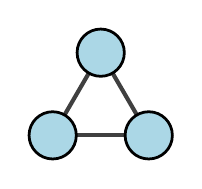
\begin{tikzpicture}
\Vertex[x=0.00, y=0.70]{0}
\Vertex[x=0.61, y=-0.35]{1}
\Vertex[x=-0.61, y=-0.35]{2}

\Edge(0)(1)
\Edge(1)(2)
\Edge(2)(0)
\end{tikzpicture}
}

\newcommand{\gsquare}{
% square
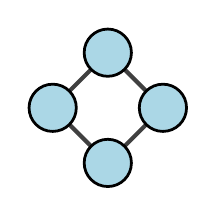
\begin{tikzpicture}
\Vertex[x=0.00, y=0.70]{0}
\Vertex[x=0.70, y=0.00]{1}
\Vertex[x=0.00, y=-0.70]{2}
\Vertex[x=-0.70, y=-0.00]{3}

\Edge(0)(1)
\Edge(1)(2)
\Edge(2)(3)
\Edge(3)(0)
\end{tikzpicture}
}
\newcommand{\gpentagon}{
% pentagon
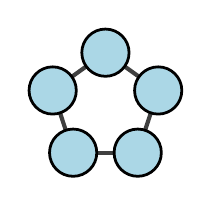
\begin{tikzpicture}
\Vertex[x=0.00, y=0.70]{0}
\Vertex[x=0.67, y=0.22]{1}
\Vertex[x=0.41, y=-0.57]{2}
\Vertex[x=-0.41, y=-0.57]{3}
\Vertex[x=-0.67, y=0.22]{4}

\Edge(0)(1)
\Edge(1)(2)
\Edge(2)(3)
\Edge(3)(4)
\Edge(4)(0)
\end{tikzpicture}
}

\newcommand{\ghexagon}{
% hexagon
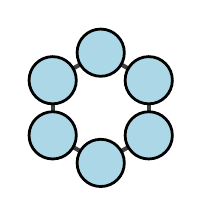
\begin{tikzpicture}
\Vertex[x=0.00, y=0.70]{0}
\Vertex[x=0.61, y=0.35]{1}
\Vertex[x=0.61, y=-0.35]{2}
\Vertex[x=0.00, y=-0.70]{3}
\Vertex[x=-0.61, y=-0.35]{4}
\Vertex[x=-0.61, y=0.35]{5}

\Edge(0)(1)
\Edge(1)(2)
\Edge(2)(3)
\Edge(3)(4)
\Edge(4)(5)
\Edge(5)(0)
\end{tikzpicture}
}

\newcommand{\gseptagon}{
% septagon
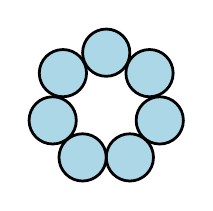
\begin{tikzpicture}
\Vertex[x=0.00, y=0.70]{0}
\Vertex[x=0.55, y=0.44]{1}
\Vertex[x=0.68, y=-0.16]{2}
\Vertex[x=0.30, y=-0.63]{3}
\Vertex[x=-0.30, y=-0.63]{4}
\Vertex[x=-0.68, y=-0.16]{5}
\Vertex[x=-0.55, y=0.44]{6}

\Edge(0)(1)
\Edge(1)(2)
\Edge(2)(3)
\Edge(3)(4)
\Edge(4)(5)
\Edge(5)(6)
\Edge(6)(0)
\end{tikzpicture}
}

\newcommand{\goctagon}{
% octagon
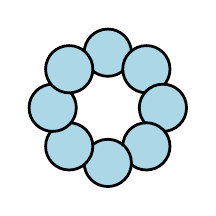
\begin{tikzpicture}
\Vertex[x=0.00, y=0.70]{0}
\Vertex[x=0.49, y=0.49]{1}
\Vertex[x=0.70, y=0.00]{2}
\Vertex[x=0.49, y=-0.49]{3}
\Vertex[x=0.00, y=-0.70]{4}
\Vertex[x=-0.49, y=-0.49]{5}
\Vertex[x=-0.70, y=-0.00]{6}
\Vertex[x=-0.49, y=0.49]{7}

\Edge(0)(1)
\Edge(1)(2)
\Edge(2)(3)
\Edge(3)(4)
\Edge(4)(5)
\Edge(5)(6)
\Edge(6)(7)
\Edge(7)(0)

\end{tikzpicture}
}


% graphs
% 8 17 7 12 7 10
% lcc
% 6 16 7 11 7 10

\newcommand{\cyclesubgraphs}{
\begin{tabular}{c c c c c c}
    \gtriangle & \gsquare & \gpentagon & \ghexagon & \gseptagon & \goctagon \\
     $8$ & $17$ & $7$ & $12$ & $7$ & $10$ 
\end{tabular}
}


\newcommand{\cyclesubgraphslcc}{
\begin{tabular}{c c c c c c}
    \gtriangle & \gsquare & \gpentagon & \ghexagon & \gseptagon & \goctagon \\
     $6 \hspace{4pt} | \hspace{4pt} \textcolor{TwitterBlue}{3}$ & $16 \hspace{4pt} | \hspace{4pt} \textcolor{TwitterBlue}{4}$ & $7 \hspace{4pt} | \hspace{4pt} \textcolor{TwitterBlue}{4}$ & $11 \hspace{4pt} | \hspace{4pt} \textcolor{TwitterBlue}{4}$ & $7 \hspace{4pt} | \hspace{4pt} \textcolor{TwitterBlue}{4}$ & $10 \hspace{4pt} | \hspace{4pt} \textcolor{TwitterBlue}{4}$ 
\end{tabular}
}


\cyclesubgraphslcc

    \caption{The figure shows the cyclic subgraphs identified within the largest connected components of user graphs, ranging from a triangle to an octagon. The numbers beneath denote the support of the subgraph in TikTok and Twitter in that order.}
    \label{fig:cycle_subgraphs}
\end{figure}


Given that cycles are not present in any mined subgraph, the complete subgraph hierarchy of up to six vertices can be mapped out, as presented in Figure \ref{fig:subgraph_hierarchy}. From it, the hierarchy of subgraphs is apparent, illustrating how the support of any child subgraph is at most equal to its parent. We see that stars and star-like patterns generally have slightly higher support than chains and chain-like patterns. Furthermore, we note that, without cycles, any mined subgraph will always be an interpolation between stars and chains.

\begin{figure}[!htbp]
    \centering
    \SetVertexStyle[Shape=circle, InnerSep=1, MinSize=4, FillColor=black, LineColor=black]
\SetEdgeStyle[Color=gray, Arrow=-stealth]

\newcommand{\dyad}{
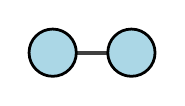
\begin{tikzpicture}
	\Vertex[x=0, y=0]{0}
    \Vertex[x=1, y=0]{1}
    \Edge[](0)(1)
\end{tikzpicture}
}

\newcommand{\triad}{
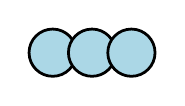
\begin{tikzpicture}
	\Vertex[x=0, y=0]{0}
    \Vertex[x=0.5, y=0]{1}
    \Vertex[x=1, y=0]{2}
    \Edge[](0)(1)
    \Edge[](1)(2)
\end{tikzpicture}
}

\newcommand{\threechain}{
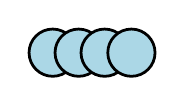
\begin{tikzpicture}
	\Vertex[x=0, y=0]{0}
    \Vertex[x=0.33, y=0]{1}
    \Vertex[x=0.66, y=0]{2}
    \Vertex[x=1, y=0]{3}
    \Edge[](0)(1)
    \Edge[](1)(2)
    \Edge[](2)(3)
\end{tikzpicture}
}

\newcommand{\threestar}{
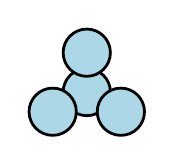
\begin{tikzpicture}
	\Vertex[x=0, y=0]{0}
    \Vertex[x=0, y=0.5]{1}
    \Vertex[x=-0.433, y=-0.25]{2}
    \Vertex[x=0.433, y=-0.25]{3}
    \Edge[](1)(0)
    \Edge[](2)(0)
    \Edge[](3)(0)
\end{tikzpicture}
}

\newcommand{\fourchain}{
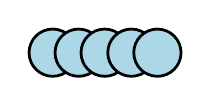
\begin{tikzpicture}
	\Vertex[x=0, y=0]{0}
    \Vertex[x=0.33, y=0]{1}
    \Vertex[x=0.66, y=0]{2}
    \Vertex[x=1, y=0]{3}
    \Vertex[x=1.33, y=0]{4}
    \Edge[](0)(1)
    \Edge[](1)(2)
    \Edge[](2)(3)
    \Edge[](3)(4)
\end{tikzpicture}
}

\newcommand{\fourstar}{
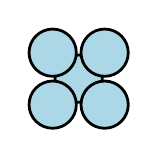
\begin{tikzpicture}
	\Vertex[x=0, y=0]{0}
    \Vertex[x=0.33, y=0.33]{1}
    \Vertex[x=0.33, y=-0.33]{2}
    \Vertex[x=-0.33, y=0.33]{3}
    \Vertex[x=-0.33, y=-0.33]{4}
    \Edge[](1)(0)
    \Edge[](2)(0)
    \Edge[](3)(0)
    \Edge[](4)(0)
\end{tikzpicture}
}

\newcommand{\starchain}{
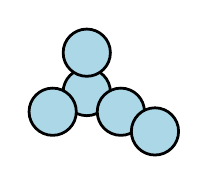
\begin{tikzpicture}
	\Vertex[x=0, y=0]{0}
    \Vertex[x=0, y=0.5]{1}
    \Vertex[x=-0.433, y=-0.25]{2}
    \Vertex[x=0.433, y=-0.25]{3}
    \Vertex[x=0.866, y=-0.5]{4}
    \Edge[](1)(0)
    \Edge[](2)(0)
    \Edge[](3)(0)
    \Edge[](4)(3)
\end{tikzpicture}
}

\newcommand{\hierarchygraph}{
\begin{tikzpicture}[node distance=2.5cm]
    % Nodes
    \node (dyad) {\makecell{\dyad\\ $36$}};
    \node (triad) [below=0.7cm of dyad] {\makecell{\triad\\ $34$}};
    \node (threechain) [below left of=triad] {\makecell{\threechain\\ $32$}};
    \node (threestar) [below right of=triad] {\makecell{\threestar\\ $33$}};
    \node (fourchain) [below left of=threechain] {\makecell{\fourchain\\ $29$}};
    \node (fourstar) [below right of=threestar] {\makecell{\fourstar\\ $32$}};
    \node (starchain) [below right of=threechain] {\makecell{\starchain\\$30$}};

    \draw (dyad) -- (triad);
    \draw (triad) -- (threechain);
    \draw (triad) -- (threestar);
    \draw (threechain) -- (fourchain);
    \draw (threechain) -- (starchain);
    \draw (threestar) -- (fourstar);
    \draw (threestar) -- (starchain);
\end{tikzpicture}
}



\newcommand{\fivechain}{
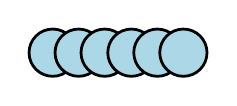
\begin{tikzpicture}
	\Vertex[x=0, y=0]{0}
	\Vertex[x=0.33, y=0]{1}
	\Vertex[x=0.66, y=0]{2}
	\Vertex[x=1, y=0]{3}
	\Vertex[x=1.33, y=0]{4}
	\Vertex[x=1.66, y=0]{5}
    \Edge[](0)(1)
    \Edge[](1)(2)
    \Edge[](2)(3)
    \Edge[](3)(4)
    \Edge[](4)(5)
\end{tikzpicture}
}

\newcommand{\threestarchain}{
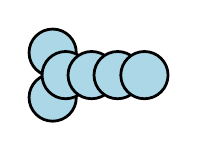
\begin{tikzpicture}
	\Vertex[x=-0.165, y=0.285]{0}
	\Vertex[x=-0.165, y=-0.285]{1}
	\Vertex[x=0, y=0]{2}
	\Vertex[x=0.33, y=0]{3}
	\Vertex[x=0.66, y=0]{4}
	\Vertex[x=1, y=0]{5}
    \Edge[](0)(2)
    \Edge[](1)(2)
    \Edge[](2)(3)
    \Edge[](3)(4)
    \Edge[](4)(5)
\end{tikzpicture}
}

\newcommand{\twothreestarchain}{
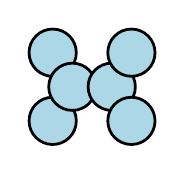
\begin{tikzpicture}
	\Vertex[x=-0.25, y=0.433]{0}
	\Vertex[x=-0.25, y=-0.433]{1}
	\Vertex[x=0, y=0]{2}
	\Vertex[x=0.5, y=0]{3}
	\Vertex[x=0.75, y=-0.433]{4}
	\Vertex[x=0.75, y=0.433]{5}
    \Edge[](0)(2)
    \Edge[](1)(2)
    \Edge[](2)(3)
    \Edge[](3)(4)
    \Edge[](3)(5)
\end{tikzpicture}
}

\newcommand{\threestartwochainz}{
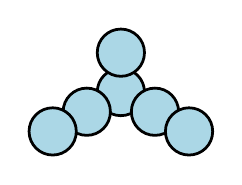
\begin{tikzpicture}
	\Vertex[x=0, y=0]{0}
    \Vertex[x=0, y=0.5]{1}
    \Vertex[x=-0.433, y=-0.25]{2}
    \Vertex[x=0.433, y=-0.25]{3}
    \Vertex[x=0.866, y=-0.5]{4}
    \Vertex[x=-0.866, y=-0.5]{5}
    \Edge[](1)(0)
    \Edge[](2)(0)
    \Edge[](3)(0)
    \Edge[](4)(3)
    \Edge[](5)(2)
\end{tikzpicture}
}

\newcommand{\fourstarchain}{
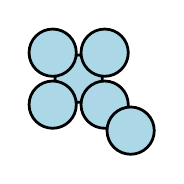
\begin{tikzpicture}
	\Vertex[x=0, y=0]{0}
    \Vertex[x=0.33, y=0.33]{1}
    \Vertex[x=0.33, y=-0.33]{2}
    \Vertex[x=-0.33, y=0.33]{3}
    \Vertex[x=-0.33, y=-0.33]{4}
    \Vertex[x=0.66, y=-0.66]{5}
    \Edge[](1)(0)
    \Edge[](2)(0)
    \Edge[](3)(0)
    \Edge[](4)(0)
    \Edge[](5)(2)
\end{tikzpicture}
}

\newcommand{\fivestar}{
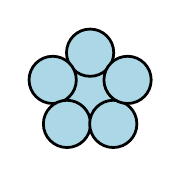
\begin{tikzpicture}
	\Vertex[x=0, y=0]{0}
    \Vertex[x=0, y=0.5]{1}
    \Vertex[x=-0.47552825814757677, y=0.15450849718747373]{2}
    \Vertex[x=-0.2938926261462366, y=-0.40450849718747367]{3}
    \Vertex[x=0.2938926261462365, y=-0.4045084971874738]{4}
    \Vertex[x=0.4755282581475768, y=0.15450849718747361]{5}
    \Edge[](1)(0)
    \Edge[](2)(0)
    \Edge[](3)(0)
    \Edge[](4)(0)
    \Edge[](5)(0)
\end{tikzpicture}
}

\newcommand{\hierarchygraphbig}{
\begin{tikzpicture}[node distance=2.5cm]
    % Nodes
    \node (dyad) {\makecell{\dyad\\ $36$}};
    \node (triad) [below=0.7cm of dyad] {\makecell{\triad\\ $34$}};
    \node (threechain) [below left of=triad] {\makecell{\threechain\\ $32$}};
    \node (threestar) [below right of=triad] {\makecell{\threestar\\ $33$}};
    \node (fourchain) [below left of=threechain] {\makecell{\fourchain\\ $29$}};
    \node (fourstar) [below right of=threestar] {\makecell{\fourstar\\ $32$}};
    \node (starchain) [below right of=threechain] {\makecell{\starchain\\$30$}};
    \node (fivechain) [below left of=fourchain] {\makecell{\fivechain\\ $27$}};
    \node (threestarchain) [below of=fourchain] {\makecell{\threestarchain\\ $28$}};
    \node (twothreestarchain) [below left=2cm and 0cm of starchain] {\makecell{\twothreestarchain\\ $25$}};
    \node (threestartwochainz) [below right=2cm and 0cm of starchain] {\makecell{\threestartwochainz\\ $28$}};
    \node (fourstarchain) [below of=fourstar] {\makecell{\fourstarchain\\ $28$}};
    \node (fivestar) [below right of=fourstar] {\makecell{\fivestar\\ $32$}};

    \draw (dyad) -- (triad);
    \draw (triad) -- (threechain);
    \draw (triad) -- (threestar);
    \draw (threechain) -- (fourchain);
    \draw (threechain) -- (starchain);
    \draw (threestar) -- (fourstar);
    \draw (threestar) -- (starchain);
    \draw (fourchain) -- (fivechain);
    \draw (fourchain) -- (threestarchain);
    \draw (starchain) -- (threestarchain);
    \draw (starchain) -- (twothreestarchain);
    \draw (starchain) -- (threestartwochainz);
    \draw (starchain) -- (fourstarchain);
    \draw (fourstar) -- (fourstarchain);
    \draw (fourstar) -- (fivestar);
    
\end{tikzpicture}
}

\newcommand{\hierarchygraphlccbig}{
\begin{tikzpicture}[node distance=2.5cm]
    % Nodes
    \node (dyad) {\makecell{\dyad\\ $36 \hspace{4pt} | \hspace{4pt} \textcolor{TwitterBlue}{6}$}};
    \node (triad) [below=0.7cm of dyad] {\makecell{\triad\\ $34 \hspace{4pt} | \hspace{4pt} \textcolor{TwitterBlue}{6}$}};
    \node (threechain) [below left of=triad] {\makecell{\threechain\\ $29 \hspace{4pt} | \hspace{4pt} \textcolor{TwitterBlue}{5}$}};
    \node (threestar) [below right of=triad] {\makecell{\threestar\\ $33 \hspace{4pt} | \hspace{4pt} \textcolor{TwitterBlue}{6}$}};
    \node (fourchain) [below left of=threechain] {\makecell{\fourchain\\ $26 \hspace{4pt} | \hspace{4pt} \textcolor{TwitterBlue}{5}$}};
    \node (fourstar) [below right of=threestar] {\makecell{\fourstar\\ $32 \hspace{4pt} | \hspace{4pt} \textcolor{TwitterBlue}{5}$}};
    \node (starchain) [below right of=threechain] {\makecell{\starchain\\$28 \hspace{4pt} | \hspace{4pt} \textcolor{TwitterBlue}{5}$}};
    \node (fivechain) [below left of=fourchain] {\makecell{\fivechain\\ $24 \hspace{4pt} | \hspace{4pt} \textcolor{TwitterBlue}{5}$}};
    \node (threestarchain) [below of=fourchain] {\makecell{\threestarchain\\ $26 \hspace{4pt} | \hspace{4pt} \textcolor{TwitterBlue}{5}$}};
    \node (threestartwochainz) [below left=2cm and 0cm of starchain] {\makecell{\threestartwochainz\\ $24 \hspace{4pt} | \hspace{4pt} \textcolor{TwitterBlue}{5}$}};
    \node (twothreestarchain) [below right=2cm and 0cm of starchain] {\makecell{\twothreestarchain\\ $22 \hspace{4pt} | \hspace{4pt} \textcolor{TwitterBlue}{5}$}};
    \node (fourstarchain) [below of=fourstar] {\makecell{\fourstarchain\\ $27 \hspace{4pt} | \hspace{4pt} \textcolor{TwitterBlue}{4}$}};
    \node (fivestar) [below right of=fourstar] {\makecell{\fivestar\\ $32 \hspace{4pt} | \hspace{4pt} \textcolor{TwitterBlue}{5}$}};

    \draw (dyad) -- (triad);
    \draw (triad) -- (threechain);
    \draw (triad) -- (threestar);
    \draw (threechain) -- (fourchain);
    \draw (threechain) -- (starchain);
    \draw (threestar) -- (fourstar);
    \draw (threestar) -- (starchain);
    \draw (fourchain) -- (fivechain);
    \draw (fourchain) -- (threestarchain);
    \draw (starchain) -- (threestarchain);
    \draw (starchain) -- (twothreestarchain);
    \draw (starchain) -- (threestartwochainz);
    \draw (starchain) -- (fourstarchain);
    \draw (fourstar) -- (fourstarchain);
    \draw (fourstar) -- (fivestar);
    
\end{tikzpicture}
}


\hierarchygraphlccbig
    \caption{The figure shows the frequent undirected subgraphs identified in TikTok user graphs using gSpan on the largest connected component. The lines between subgraphs illustrate their hierarchical relationships, where each subgraph extends from the one above. The numbers are the supports of the given subgraphs in TikTok and Twitter respectively. Simpler structures, such as dyads $S_1$ ($support=36$), form the foundation, while more complex patterns like chains and star-like structures emerge as extensions with lower support. This highlights how TikTok stitch patterns evolve, often around central hubs or sequential interactions.}
    \label{fig:subgraph_hierarchy}
\end{figure}

These findings are also true going beyond subgraphs with six vertices, as seen in Figure \ref{fig:large_subgraphs}. The most common substructure with more than six vertices is a six-star $S_6$, which appears in $29$ user graphs' largest weak component. This aligns with the notion of central users often acting as hubs, either for generating reactions or being highly active in reacting to others. This is a general trend for most of the subgraphs, with pure stars having higher support than pure chains. In fact, for subgraphs where $|V| \geq 8$, the pure chain does not appear within the mined set of graphs with a minimum support threshold of $21$. The rest of the subgraphs are somewhere in between stars and chains, often occurring in the form of stars extended with a chain, or a chain connecting two stars. The support for these interpolations appears to correlate with the degree to which they resemble a star or a chain. By comparison, the chains' support is generally equal to the stars' support in Twitter networks, indicating a preference for chains when compared to TikTok.

\begin{figure}[!htbp]
    \centering
    \begin{adjustwidth}{-\textwidth}{-\textwidth}
        \centering    
        \input{figures/5 results/large_subgraphs}
    \end{adjustwidth}
    \caption{The figure displays frequent subgraphs with seven or more nodes in the user graphs, grouped by their number their number of vertices $|V|$, down to support threshold $22$ (see the full figure in Appendix \ref{lab:fsm_appendix} Table \ref{fig:large_subgraphs_full}). The numbers are the support in TikTok and Twitter respectively. Generally, stars and star-like patterns are the most common for each size, with chains and chain-like patterns having systematically lower supports.}
    \label{fig:large_subgraphs}
\end{figure}

Nuancing the subgraphs with direction provides further insight into the tendencies in stitch behavior. As reflected by the lack of odd-numbered cycles, a user being both stitched and stitching another user is rare. This is further reinforced by the directed subgraphs in Figure \ref{fig:directed_subgraphs}, showing an out-two-star has support $34$, an in-two-star has support $33$, but a mixed-direction two-star has support $22$, meaning it is comparatively uncommon for a user to both stitch and be stitched. The same trend is reflected in all larger structures, with three-stars $S_3$ having out-star support $32$, in-star support $31$ and mixed-star support $17$ or $14$ based on the specific directionality. Conversely, Twitter exhibits relatively uniform levels of support across in-, out- and mixed-direction two-stars $S_2$. Moreover, three-stars $S_3$ display interesting supports. Although the in- and out-three-star $S_3$ Twitter support is comparable, the two mixed-direction three-stars $S_3$ vary greatly compared to all previous Twitter support patterns. 

From the figure, the square from above is also specified with direction. As hypothesized, the square consists of two users collectively stitching two other users, forming a weak cycle. This pattern has equivalent support with the undirected square, and no other directed squares are mined, leading to this structure largely explaining the undirected squares support. 

\begin{figure}[h]
    \centering
    \begin{adjustwidth}{-\textwidth}{-\textwidth}
        \centering
        \setlength{\tabcolsep}{9pt}
\begin{tabular}{ccccccccc}
$|V| = 3$&\makecell{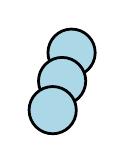
\begin{tikzpicture}
	\Vertex[x=0.06, y=0.50]{0}
	\Vertex[x=-0.06, y=0.14]{1}
	\Vertex[x=-0.18, y=-0.23]{2}
	\Edge[color=gray,Direct](0)(1)
	\Edge[color=gray,Direct](2)(1)
\end{tikzpicture}
\\$32 \hspace{4pt} | \hspace{4pt} \textcolor{TwitterBlue}{5}$
}
&\makecell{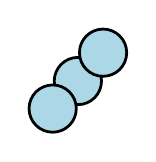
\begin{tikzpicture}
	\Vertex[x=0.18, y=0.02]{0}
	\Vertex[x=0.50, y=0.38]{1}
	\Vertex[x=-0.14, y=-0.33]{2}
	\Edge[color=gray,Direct](0)(1)
	\Edge[color=gray,Direct](0)(2)
\end{tikzpicture}
\\$31 \hspace{4pt} | \hspace{4pt} \textcolor{TwitterBlue}{6}$
}
&\makecell{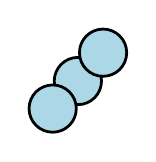
\begin{tikzpicture}
	\Vertex[x=0.18, y=0.02]{0}
	\Vertex[x=0.50, y=0.38]{1}
	\Vertex[x=-0.14, y=-0.33]{2}
	\Edge[color=gray,Direct](0)(1)
	\Edge[color=gray,Direct](2)(0)
\end{tikzpicture}
\\$16 \hspace{4pt} | \hspace{4pt} \textcolor{TwitterBlue}{5}$
}
\\[0.9cm]
$|V| = 4$&\makecell{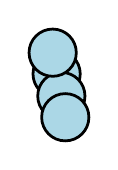
\begin{tikzpicture}
	\Vertex[x=0.04, y=0.05]{0}
	\Vertex[x=0.10, y=-0.23]{1}
	\Vertex[x=-0.01, y=0.32]{2}
	\Vertex[x=0.15, y=-0.50]{3}
	\Edge[color=gray,Direct](0)(1)
	\Edge[color=gray,Direct](0)(2)
	\Edge[color=gray,Direct](3)(1)
\end{tikzpicture}
\\$29 \hspace{4pt} | \hspace{4pt} \textcolor{TwitterBlue}{5}$
}
&\makecell{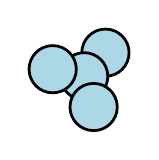
\begin{tikzpicture}
	\Vertex[x=0.17, y=0.49]{0}
	\Vertex[x=-0.10, y=0.19]{1}
	\Vertex[x=-0.50, y=0.28]{2}
	\Vertex[x=0.02, y=-0.20]{3}
	\Edge[color=gray,Direct](0)(1)
	\Edge[color=gray,Direct](2)(1)
	\Edge[color=gray,Direct](3)(1)
\end{tikzpicture}
\\$28 \hspace{4pt} | \hspace{4pt} \textcolor{TwitterBlue}{5}$
}
&\makecell{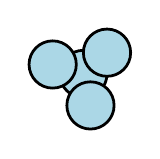
\begin{tikzpicture}
	\Vertex[x=0.19, y=-0.10]{0}
	\Vertex[x=0.49, y=0.17]{1}
	\Vertex[x=-0.20, y=0.02]{2}
	\Vertex[x=0.28, y=-0.50]{3}
	\Edge[color=gray,Direct](0)(1)
	\Edge[color=gray,Direct](0)(2)
	\Edge[color=gray,Direct](0)(3)
\end{tikzpicture}
\\$27 \hspace{4pt} | \hspace{4pt} \textcolor{TwitterBlue}{6}$
}
&\makecell{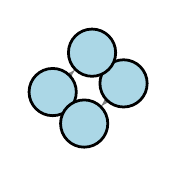
\begin{tikzpicture}
	\Vertex[x=0.40, y=0.11]{0}
	\Vertex[x=-0.00, y=0.50]{1}
	\Vertex[x=-0.50, y=-0.00]{2}
	\Vertex[x=-0.10, y=-0.40]{3}
	\Edge[color=gray,Direct](0)(1)
	\Edge[color=gray,Direct](0)(3)
	\Edge[color=gray,Direct](2)(3)
	\Edge[color=gray,Direct](2)(1)
\end{tikzpicture}
\\$16 \hspace{4pt} | \hspace{4pt} \textcolor{TwitterBlue}{4}$
}
&\makecell{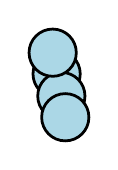
\begin{tikzpicture}
	\Vertex[x=0.04, y=0.05]{0}
	\Vertex[x=0.10, y=-0.23]{1}
	\Vertex[x=-0.01, y=0.32]{2}
	\Vertex[x=0.15, y=-0.50]{3}
	\Edge[color=gray,Direct](0)(1)
	\Edge[color=gray,Direct](0)(2)
	\Edge[color=gray,Direct](1)(3)
\end{tikzpicture}
\\$14 \hspace{4pt} | \hspace{4pt} \textcolor{TwitterBlue}{5}$
}
&\makecell{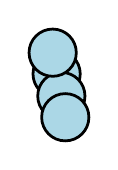
\begin{tikzpicture}
	\Vertex[x=0.04, y=0.05]{0}
	\Vertex[x=0.10, y=-0.23]{1}
	\Vertex[x=-0.01, y=0.32]{2}
	\Vertex[x=0.15, y=-0.50]{3}
	\Edge[color=gray,Direct](0)(1)
	\Edge[color=gray,Direct](2)(0)
	\Edge[color=gray,Direct](3)(1)
\end{tikzpicture}
\\$14 \hspace{4pt} | \hspace{4pt} \textcolor{TwitterBlue}{5}$
}
&\makecell{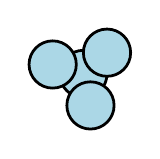
\begin{tikzpicture}
	\Vertex[x=0.19, y=-0.10]{0}
	\Vertex[x=0.49, y=0.17]{1}
	\Vertex[x=-0.20, y=0.02]{2}
	\Vertex[x=0.28, y=-0.50]{3}
	\Edge[color=gray,Direct](0)(1)
	\Edge[color=gray,Direct](0)(2)
	\Edge[color=gray,Direct](3)(0)
\end{tikzpicture}
\\$13 \hspace{4pt} | \hspace{4pt} \textcolor{TwitterBlue}{4}$
}
&\makecell{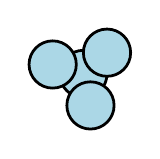
\begin{tikzpicture}
	\Vertex[x=0.19, y=-0.10]{0}
	\Vertex[x=0.49, y=0.17]{1}
	\Vertex[x=-0.20, y=0.02]{2}
	\Vertex[x=0.28, y=-0.50]{3}
	\Edge[color=gray,Direct](0)(1)
	\Edge[color=gray,Direct](2)(0)
	\Edge[color=gray,Direct](3)(0)
\end{tikzpicture}
\\$13 \hspace{4pt} | \hspace{4pt} \textcolor{TwitterBlue}{1}$
}
\end{tabular}

    \end{adjustwidth}
    \caption{The figure shows the frequent directed subgraphs identified in the user graphs. Due to computational constraints, the analysis was limited to subgraphs with four or fewer nodes.
    We observe that chains and star structures with mixed direction occurs a lot less frequently than those with consistent directionality.} 
    \label{fig:directed_subgraphs}
\end{figure}

% Something something motifs

To determine whether any mined subgraph is a motif, subgraphs are compared to relevant null models. Doing this did not reveal significant motifs for undirected and directed subgraph mining. This result is likely due to the choice of null model, the simplicity of the mined subgraphs, and the specific support definition. Configuration models preserve the degree distribution, and many of the simple structures are explained by the degree distribution. For instance, stars can be entirely explained by the degree distribution: high-degree central nodes and low-degree peripheral nodes (each with an out-degree of $1$) will occur with equal prevalence in a configuration model. Other mined subgraphs are often star-like patterns, and in combination with the large size of many user graphs, the subgraphs are likely to emerge by chance based on the given degree distribution. This is further perpetuated by the support definition. Each subgraph only has to appear once for it to count towards the support, meaning the support definition does not account for differences in frequency within the user graphs and configuration models.   

% However, our analysis does not reveal significant motifs within the TikTok stitch networks. This result is likely due to the dominant star-like structures characteristic of these graphs. Configuration models preserve the degree distribution, and in the case of star structures, the high-degree central nodes (representing hubs) and low-degree peripheral nodes (degree of 1) are maintained. This results in similar subgraph occurrences between the observed graphs and the configuration models, making it challenging to identify motifs that exceed the baseline expectations.


\subsection{Sentiment Subgraphs}

Adding sentiment as a dimension yields the subgraphs illustrated in Figure \ref{fig:sentiment_subgraphs}. From these we see that positive and negative edges have a support of $30$, missing sentiment edges $27$, and neutral edges $22$. An explanation for the maximum support of $30$ lies in the size of the largest components, as ten user graphs have a largest component size of $|V_{lcc}| \leq 11$. Outside of these surface-level observations, no clear trends emerge with regard to sentiment patterns. 

A notable observation is the lack of anything between pure stars and chains, unlike in the previous subgraph mining. In fact, subgraphs with $|V| \geq 5$ consist of purely stars, further indicating that TikTok stitch networks are dominated by this pattern. Although no mechanism prevents other subgraphs from appearing, the likely reason for their absence is the increased number of possible subgraphs, especially due to the limited largest component sizes. As four new edge classes are introduced, the possible subgraphs increase exponentially.  

\begin{figure}[h]
    \centering
    \begin{adjustwidth}{-\textwidth}{-\textwidth}
        \centering
        \setlength{\tabcolsep}{9pt}
\begin{tabular}{ccccccccc}
$|V| = 2$&\makecell{\begin{tikzpicture}
	\Vertex[x=0.50, y=-0.00]{0}
	\Vertex[x=-0.28, y=0.00]{1}
	\Edge[color=SentimentPositive](0)(1)
\end{tikzpicture}
\\$30 \hspace{4pt} | \hspace{4pt} \textcolor{TwitterBlue}{6}$
}
&\makecell{\begin{tikzpicture}
	\Vertex[x=0.50, y=-0.00]{0}
	\Vertex[x=-0.28, y=0.00]{1}
	\Edge[color=SentimentNegative](0)(1)
\end{tikzpicture}
\\$30 \hspace{4pt} | \hspace{4pt} \textcolor{TwitterBlue}{5}$
}
&\makecell{\begin{tikzpicture}
	\Vertex[x=0.50, y=-0.00]{0}
	\Vertex[x=-0.28, y=0.00]{1}
	\Edge[color=SentimentMissing](0)(1)
\end{tikzpicture}
\\$27 \hspace{4pt} | \hspace{4pt} \textcolor{TwitterBlue}{-}$
}
&\makecell{\begin{tikzpicture}
	\Vertex[x=0.50, y=-0.00]{0}
	\Vertex[x=-0.28, y=0.00]{1}
	\Edge[color=SentimentNeutral](0)(1)
\end{tikzpicture}
\\$22 \hspace{4pt} | \hspace{4pt} \textcolor{TwitterBlue}{5}$
}
\\[0.9cm]
$|V| = 3$&\makecell{\begin{tikzpicture}
	\Vertex[x=0.06, y=0.50]{0}
	\Vertex[x=-0.06, y=0.14]{1}
	\Vertex[x=-0.18, y=-0.23]{2}
	\Edge[color=SentimentPositive](0)(1)
	\Edge[color=SentimentNegative](1)(2)
\end{tikzpicture}
\\$28 \hspace{4pt} | \hspace{4pt} \textcolor{TwitterBlue}{5}$
}
&\makecell{\begin{tikzpicture}
	\Vertex[x=0.06, y=0.50]{0}
	\Vertex[x=-0.06, y=0.14]{1}
	\Vertex[x=-0.18, y=-0.23]{2}
	\Edge[color=SentimentNegative](0)(1)
	\Edge[color=SentimentNegative](1)(2)
\end{tikzpicture}
\\$28 \hspace{4pt} | \hspace{4pt} \textcolor{TwitterBlue}{5}$
}
&\makecell{\begin{tikzpicture}
	\Vertex[x=0.06, y=0.50]{0}
	\Vertex[x=-0.06, y=0.14]{1}
	\Vertex[x=-0.18, y=-0.23]{2}
	\Edge[color=SentimentPositive](0)(1)
	\Edge[color=SentimentPositive](1)(2)
\end{tikzpicture}
\\$28 \hspace{4pt} | \hspace{4pt} \textcolor{TwitterBlue}{4}$
}
&\makecell{\begin{tikzpicture}
	\Vertex[x=0.06, y=0.50]{0}
	\Vertex[x=-0.06, y=0.14]{1}
	\Vertex[x=-0.18, y=-0.23]{2}
	\Edge[color=SentimentMissing](0)(1)
	\Edge[color=SentimentMissing](1)(2)
\end{tikzpicture}
\\$25 \hspace{4pt} | \hspace{4pt} \textcolor{TwitterBlue}{-}$
}
&\makecell{\begin{tikzpicture}
	\Vertex[x=0.06, y=0.50]{0}
	\Vertex[x=-0.06, y=0.14]{1}
	\Vertex[x=-0.18, y=-0.23]{2}
	\Edge[color=SentimentNeutral](0)(1)
	\Edge[color=SentimentPositive](1)(2)
\end{tikzpicture}
\\$22 \hspace{4pt} | \hspace{4pt} \textcolor{TwitterBlue}{5}$
}
&\makecell{\begin{tikzpicture}
	\Vertex[x=0.06, y=0.50]{0}
	\Vertex[x=-0.06, y=0.14]{1}
	\Vertex[x=-0.18, y=-0.23]{2}
	\Edge[color=SentimentNeutral](0)(1)
	\Edge[color=SentimentNegative](1)(2)
\end{tikzpicture}
\\$22 \hspace{4pt} | \hspace{4pt} \textcolor{TwitterBlue}{4}$
}
&\makecell{\begin{tikzpicture}
	\Vertex[x=0.06, y=0.50]{0}
	\Vertex[x=-0.06, y=0.14]{1}
	\Vertex[x=-0.18, y=-0.23]{2}
	\Edge[color=SentimentPositive](0)(1)
	\Edge[color=SentimentMissing](1)(2)
\end{tikzpicture}
\\$22 \hspace{4pt} | \hspace{4pt} \textcolor{TwitterBlue}{-}$
}
&\makecell{\begin{tikzpicture}
	\Vertex[x=0.06, y=0.50]{0}
	\Vertex[x=-0.06, y=0.14]{1}
	\Vertex[x=-0.18, y=-0.23]{2}
	\Edge[color=SentimentNegative](0)(1)
	\Edge[color=SentimentMissing](1)(2)
\end{tikzpicture}
\\$22 \hspace{4pt} | \hspace{4pt} \textcolor{TwitterBlue}{-}$
}
\\[0.9cm]
$|V| = 4$&\makecell{\begin{tikzpicture}
	\Vertex[x=0.17, y=0.49]{0}
	\Vertex[x=-0.10, y=0.19]{1}
	\Vertex[x=-0.50, y=0.28]{2}
	\Vertex[x=0.02, y=-0.20]{3}
	\Edge[color=SentimentPositive](0)(1)
	\Edge[color=SentimentPositive](1)(2)
	\Edge[color=SentimentNegative](1)(3)
\end{tikzpicture}
\\$27 \hspace{4pt} | \hspace{4pt} \textcolor{TwitterBlue}{4}$
}
&\makecell{\begin{tikzpicture}
	\Vertex[x=0.17, y=0.49]{0}
	\Vertex[x=-0.10, y=0.19]{1}
	\Vertex[x=-0.50, y=0.28]{2}
	\Vertex[x=0.02, y=-0.20]{3}
	\Edge[color=SentimentPositive](0)(1)
	\Edge[color=SentimentNegative](1)(2)
	\Edge[color=SentimentNegative](1)(3)
\end{tikzpicture}
\\$26 \hspace{4pt} | \hspace{4pt} \textcolor{TwitterBlue}{5}$
}
&\makecell{\begin{tikzpicture}
	\Vertex[x=0.17, y=0.49]{0}
	\Vertex[x=-0.10, y=0.19]{1}
	\Vertex[x=-0.50, y=0.28]{2}
	\Vertex[x=0.02, y=-0.20]{3}
	\Edge[color=SentimentPositive](0)(1)
	\Edge[color=SentimentPositive](1)(2)
	\Edge[color=SentimentPositive](1)(3)
\end{tikzpicture}
\\$25 \hspace{4pt} | \hspace{4pt} \textcolor{TwitterBlue}{4}$
}
&\makecell{\begin{tikzpicture}
	\Vertex[x=0.17, y=0.49]{0}
	\Vertex[x=-0.10, y=0.19]{1}
	\Vertex[x=-0.50, y=0.28]{2}
	\Vertex[x=0.02, y=-0.20]{3}
	\Edge[color=SentimentNegative](0)(1)
	\Edge[color=SentimentNegative](1)(2)
	\Edge[color=SentimentNegative](1)(3)
\end{tikzpicture}
\\$22 \hspace{4pt} | \hspace{4pt} \textcolor{TwitterBlue}{5}$
}
&\makecell{\begin{tikzpicture}
	\Vertex[x=0.17, y=0.49]{0}
	\Vertex[x=-0.10, y=0.19]{1}
	\Vertex[x=-0.50, y=0.28]{2}
	\Vertex[x=0.02, y=-0.20]{3}
	\Edge[color=SentimentNeutral](0)(1)
	\Edge[color=SentimentPositive](1)(2)
	\Edge[color=SentimentPositive](1)(3)
\end{tikzpicture}
\\$22 \hspace{4pt} | \hspace{4pt} \textcolor{TwitterBlue}{4}$
}
&\makecell{\begin{tikzpicture}
	\Vertex[x=0.17, y=0.49]{0}
	\Vertex[x=-0.10, y=0.19]{1}
	\Vertex[x=-0.50, y=0.28]{2}
	\Vertex[x=0.02, y=-0.20]{3}
	\Edge[color=SentimentNeutral](0)(1)
	\Edge[color=SentimentPositive](1)(2)
	\Edge[color=SentimentNegative](1)(3)
\end{tikzpicture}
\\$22 \hspace{4pt} | \hspace{4pt} \textcolor{TwitterBlue}{4}$
}
&\makecell{\begin{tikzpicture}
	\Vertex[x=0.17, y=0.49]{0}
	\Vertex[x=-0.10, y=0.19]{1}
	\Vertex[x=-0.50, y=0.28]{2}
	\Vertex[x=0.02, y=-0.20]{3}
	\Edge[color=SentimentPositive](0)(1)
	\Edge[color=SentimentPositive](1)(2)
	\Edge[color=SentimentMissing](1)(3)
\end{tikzpicture}
\\$22 \hspace{4pt} | \hspace{4pt} \textcolor{TwitterBlue}{-}$
}
&\makecell{\begin{tikzpicture}
	\Vertex[x=0.17, y=0.49]{0}
	\Vertex[x=-0.10, y=0.19]{1}
	\Vertex[x=-0.50, y=0.28]{2}
	\Vertex[x=0.02, y=-0.20]{3}
	\Edge[color=SentimentMissing](0)(1)
	\Edge[color=SentimentMissing](1)(2)
	\Edge[color=SentimentMissing](1)(3)
\end{tikzpicture}
\\$22 \hspace{4pt} | \hspace{4pt} \textcolor{TwitterBlue}{-}$
}
&&\makecell{\begin{tikzpicture}
	\Vertex[x=0.35, y=0.50]{0}
	\Vertex[x=0.09, y=0.18]{1}
	\Vertex[x=-0.17, y=-0.13]{2}
	\Vertex[x=-0.43, y=-0.45]{3}
	\Edge[color=SentimentPositive](0)(1)
	\Edge[color=SentimentNegative](1)(2)
	\Edge[color=SentimentNegative](2)(3)
\end{tikzpicture}
\\$21 \hspace{4pt} | \hspace{4pt} \textcolor{TwitterBlue}{5}$
}
&\makecell{\begin{tikzpicture}
	\Vertex[x=0.35, y=0.50]{0}
	\Vertex[x=0.09, y=0.18]{1}
	\Vertex[x=-0.17, y=-0.13]{2}
	\Vertex[x=-0.43, y=-0.45]{3}
	\Edge[color=SentimentPositive](0)(1)
	\Edge[color=SentimentPositive](1)(2)
	\Edge[color=SentimentPositive](2)(3)
\end{tikzpicture}
\\$21 \hspace{4pt} | \hspace{4pt} \textcolor{TwitterBlue}{4}$
}
&\makecell{\begin{tikzpicture}
	\Vertex[x=0.17, y=0.49]{0}
	\Vertex[x=-0.10, y=0.19]{1}
	\Vertex[x=-0.50, y=0.28]{2}
	\Vertex[x=0.02, y=-0.20]{3}
	\Edge[color=SentimentPositive](0)(1)
	\Edge[color=SentimentNegative](1)(2)
	\Edge[color=SentimentMissing](1)(3)
\end{tikzpicture}
\\$21 \hspace{4pt} | \hspace{4pt} \textcolor{TwitterBlue}{-}$
}
\\[0.9cm]
$|V| = 5$&\makecell{\begin{tikzpicture}
	\Vertex[x=0.31, y=0.26]{0}
	\Vertex[x=-0.04, y=0.14]{1}
	\Vertex[x=-0.16, y=0.50]{2}
	\Vertex[x=-0.40, y=0.03]{3}
	\Vertex[x=0.08, y=-0.21]{4}
	\Edge[color=SentimentPositive](0)(1)
	\Edge[color=SentimentPositive](1)(2)
	\Edge[color=SentimentNegative](1)(3)
	\Edge[color=SentimentNegative](1)(4)
\end{tikzpicture}
\\$26 \hspace{4pt} | \hspace{4pt} \textcolor{TwitterBlue}{4}$
}
&\makecell{\begin{tikzpicture}
	\Vertex[x=0.31, y=0.26]{0}
	\Vertex[x=-0.04, y=0.14]{1}
	\Vertex[x=-0.16, y=0.50]{2}
	\Vertex[x=-0.40, y=0.03]{3}
	\Vertex[x=0.08, y=-0.21]{4}
	\Edge[color=SentimentPositive](0)(1)
	\Edge[color=SentimentPositive](1)(2)
	\Edge[color=SentimentPositive](1)(3)
	\Edge[color=SentimentNegative](1)(4)
\end{tikzpicture}
\\$25 \hspace{4pt} | \hspace{4pt} \textcolor{TwitterBlue}{4}$
}
&\makecell{\begin{tikzpicture}
	\Vertex[x=0.31, y=0.26]{0}
	\Vertex[x=-0.04, y=0.14]{1}
	\Vertex[x=-0.16, y=0.50]{2}
	\Vertex[x=-0.40, y=0.03]{3}
	\Vertex[x=0.08, y=-0.21]{4}
	\Edge[color=SentimentPositive](0)(1)
	\Edge[color=SentimentPositive](1)(2)
	\Edge[color=SentimentPositive](1)(3)
	\Edge[color=SentimentPositive](1)(4)
\end{tikzpicture}
\\$24 \hspace{4pt} | \hspace{4pt} \textcolor{TwitterBlue}{4}$
}
&\makecell{\begin{tikzpicture}
	\Vertex[x=0.31, y=0.26]{0}
	\Vertex[x=-0.04, y=0.14]{1}
	\Vertex[x=-0.16, y=0.50]{2}
	\Vertex[x=-0.40, y=0.03]{3}
	\Vertex[x=0.08, y=-0.21]{4}
	\Edge[color=SentimentPositive](0)(1)
	\Edge[color=SentimentNegative](1)(2)
	\Edge[color=SentimentNegative](1)(3)
	\Edge[color=SentimentNegative](1)(4)
\end{tikzpicture}
\\$22 \hspace{4pt} | \hspace{4pt} \textcolor{TwitterBlue}{4}$
}
&\makecell{\begin{tikzpicture}
	\Vertex[x=0.31, y=0.26]{0}
	\Vertex[x=-0.04, y=0.14]{1}
	\Vertex[x=-0.16, y=0.50]{2}
	\Vertex[x=-0.40, y=0.03]{3}
	\Vertex[x=0.08, y=-0.21]{4}
	\Edge[color=SentimentNeutral](0)(1)
	\Edge[color=SentimentPositive](1)(2)
	\Edge[color=SentimentPositive](1)(3)
	\Edge[color=SentimentNegative](1)(4)
\end{tikzpicture}
\\$21 \hspace{4pt} | \hspace{4pt} \textcolor{TwitterBlue}{4}$
}
&\makecell{\begin{tikzpicture}
	\Vertex[x=0.31, y=0.26]{0}
	\Vertex[x=-0.04, y=0.14]{1}
	\Vertex[x=-0.16, y=0.50]{2}
	\Vertex[x=-0.40, y=0.03]{3}
	\Vertex[x=0.08, y=-0.21]{4}
	\Edge[color=SentimentNegative](0)(1)
	\Edge[color=SentimentNegative](1)(2)
	\Edge[color=SentimentNegative](1)(3)
	\Edge[color=SentimentNegative](1)(4)
\end{tikzpicture}
\\$21 \hspace{4pt} | \hspace{4pt} \textcolor{TwitterBlue}{4}$
}
\\[0.9cm]
$|V| = 6$&\makecell{\begin{tikzpicture}
	\Vertex[x=0.49, y=0.32]{0}
	\Vertex[x=0.16, y=0.07]{1}
	\Vertex[x=0.02, y=0.46]{2}
	\Vertex[x=-0.25, y=0.06]{3}
	\Vertex[x=0.04, y=-0.33]{4}
	\Vertex[x=0.50, y=-0.16]{5}
	\Edge[color=SentimentPositive](0)(1)
	\Edge[color=SentimentPositive](1)(2)
	\Edge[color=SentimentPositive](1)(3)
	\Edge[color=SentimentPositive](1)(4)
	\Edge[color=SentimentNegative](1)(5)
\end{tikzpicture}
\\$24 \hspace{4pt} | \hspace{4pt} \textcolor{TwitterBlue}{4}$
}
&\makecell{\begin{tikzpicture}
	\Vertex[x=0.49, y=0.32]{0}
	\Vertex[x=0.16, y=0.07]{1}
	\Vertex[x=0.02, y=0.46]{2}
	\Vertex[x=-0.25, y=0.06]{3}
	\Vertex[x=0.04, y=-0.33]{4}
	\Vertex[x=0.50, y=-0.16]{5}
	\Edge[color=SentimentPositive](0)(1)
	\Edge[color=SentimentPositive](1)(2)
	\Edge[color=SentimentPositive](1)(3)
	\Edge[color=SentimentNegative](1)(4)
	\Edge[color=SentimentNegative](1)(5)
\end{tikzpicture}
\\$23 \hspace{4pt} | \hspace{4pt} \textcolor{TwitterBlue}{4}$
}
&\makecell{\begin{tikzpicture}
	\Vertex[x=0.49, y=0.32]{0}
	\Vertex[x=0.16, y=0.07]{1}
	\Vertex[x=0.02, y=0.46]{2}
	\Vertex[x=-0.25, y=0.06]{3}
	\Vertex[x=0.04, y=-0.33]{4}
	\Vertex[x=0.50, y=-0.16]{5}
	\Edge[color=SentimentPositive](0)(1)
	\Edge[color=SentimentPositive](1)(2)
	\Edge[color=SentimentNegative](1)(3)
	\Edge[color=SentimentNegative](1)(4)
	\Edge[color=SentimentNegative](1)(5)
\end{tikzpicture}
\\$22 \hspace{4pt} | \hspace{4pt} \textcolor{TwitterBlue}{4}$
}
&\makecell{\begin{tikzpicture}
	\Vertex[x=0.49, y=0.32]{0}
	\Vertex[x=0.16, y=0.07]{1}
	\Vertex[x=0.02, y=0.46]{2}
	\Vertex[x=-0.25, y=0.06]{3}
	\Vertex[x=0.04, y=-0.33]{4}
	\Vertex[x=0.50, y=-0.16]{5}
	\Edge[color=SentimentPositive](0)(1)
	\Edge[color=SentimentPositive](1)(2)
	\Edge[color=SentimentPositive](1)(3)
	\Edge[color=SentimentPositive](1)(4)
	\Edge[color=SentimentPositive](1)(5)
\end{tikzpicture}
\\$21 \hspace{4pt} | \hspace{4pt} \textcolor{TwitterBlue}{4}$
}
&\makecell{\begin{tikzpicture}
	\Vertex[x=0.49, y=0.32]{0}
	\Vertex[x=0.16, y=0.07]{1}
	\Vertex[x=0.02, y=0.46]{2}
	\Vertex[x=-0.25, y=0.06]{3}
	\Vertex[x=0.04, y=-0.33]{4}
	\Vertex[x=0.50, y=-0.16]{5}
	\Edge[color=SentimentPositive](0)(1)
	\Edge[color=SentimentNegative](1)(2)
	\Edge[color=SentimentNegative](1)(3)
	\Edge[color=SentimentNegative](1)(4)
	\Edge[color=SentimentNegative](1)(5)
\end{tikzpicture}
\\$21 \hspace{4pt} | \hspace{4pt} \textcolor{TwitterBlue}{4}$
}
\\[0.9cm]
$|V| = 7$&\makecell{\begin{tikzpicture}
	\Vertex[x=-0.50, y=-0.14]{0}
	\Vertex[x=-0.21, y=-0.13]{1}
	\Vertex[x=-0.34, y=-0.39]{2}
	\Vertex[x=-0.37, y=0.11]{3}
	\Vertex[x=-0.05, y=-0.37]{4}
	\Vertex[x=-0.08, y=0.13]{5}
	\Vertex[x=0.08, y=-0.11]{6}
	\Edge[color=SentimentPositive](0)(1)
	\Edge[color=SentimentPositive](1)(2)
	\Edge[color=SentimentPositive](1)(3)
	\Edge[color=SentimentPositive](1)(4)
	\Edge[color=SentimentPositive](1)(5)
	\Edge[color=SentimentNegative](1)(6)
\end{tikzpicture}
\\$21 \hspace{4pt} | \hspace{4pt} \textcolor{TwitterBlue}{4}$
}
&\makecell{\begin{tikzpicture}
	\Vertex[x=-0.50, y=-0.14]{0}
	\Vertex[x=-0.21, y=-0.13]{1}
	\Vertex[x=-0.34, y=-0.39]{2}
	\Vertex[x=-0.37, y=0.11]{3}
	\Vertex[x=-0.05, y=-0.37]{4}
	\Vertex[x=-0.08, y=0.13]{5}
	\Vertex[x=0.08, y=-0.11]{6}
	\Edge[color=SentimentPositive](0)(1)
	\Edge[color=SentimentPositive](1)(2)
	\Edge[color=SentimentNegative](1)(3)
	\Edge[color=SentimentNegative](1)(4)
	\Edge[color=SentimentNegative](1)(5)
	\Edge[color=SentimentNegative](1)(6)
\end{tikzpicture}
\\$21 \hspace{4pt} | \hspace{4pt} \textcolor{TwitterBlue}{4}$
}
\end{tabular}

    \end{adjustwidth}
    \caption{The subgraphs identified in Figure \ref{fig:subgraph_hierarchy}, enriched with sentiment labels. Green edges represent \textcolor{SentimentPositive}{positive} sentiments, red for \textcolor{SentimentNegative}{negative}, gray for \textcolor{SentimentNeutral}{neutral}, and blue for \textcolor{SentimentMissing}{missing} sentiments. The subgraphs highlight how sentiment influences the structure of user interactions. Star-like structural patterns dominate, reflecting either central user receiving reactions, or a central user reacting. If a subgraph contains a \textcolor{SentimentMissing}{missing} sentiment edge, the Twitter support is undefined.}
    \label{fig:sentiment_subgraphs}
\end{figure}

Building on the undirected sentiment subgraphs, Figure \ref{fig:sentiment_directed} introduces directionality as an additional dimension. However, no new unexpected patterns emerge with regard to the combination of sentiment and direction. 

\begin{figure}[h]
    \centering
    \begin{adjustwidth}{-\textwidth}{-\textwidth}
        \centering
        \setlength{\tabcolsep}{9pt}
\begin{tabular}{cccccccccc}
$|V| = 2$&\makecell{\begin{tikzpicture}
	\Vertex[x=0.50, y=-0.00]{0}
	\Vertex[x=-0.28, y=0.00]{1}
	\Edge[color=SentimentPositive,Direct](0)(1)
\end{tikzpicture}
\\$30 \hspace{4pt} | \hspace{4pt} \textcolor{TwitterBlue}{6}$
}
&\makecell{\begin{tikzpicture}
	\Vertex[x=0.50, y=-0.00]{0}
	\Vertex[x=-0.28, y=0.00]{1}
	\Edge[color=SentimentNegative,Direct](0)(1)
\end{tikzpicture}
\\$30 \hspace{4pt} | \hspace{4pt} \textcolor{TwitterBlue}{5}$
}
&\makecell{\begin{tikzpicture}
	\Vertex[x=0.50, y=-0.00]{0}
	\Vertex[x=-0.28, y=0.00]{1}
	\Edge[color=SentimentMissing,Direct](0)(1)
\end{tikzpicture}
\\$27 \hspace{4pt} | \hspace{4pt} \textcolor{TwitterBlue}{-}$
}
&\makecell{\begin{tikzpicture}
	\Vertex[x=0.50, y=-0.00]{0}
	\Vertex[x=-0.28, y=0.00]{1}
	\Edge[color=SentimentNeutral,Direct](0)(1)
\end{tikzpicture}
\\$22 \hspace{4pt} | \hspace{4pt} \textcolor{TwitterBlue}{5}$
}
\\[0.9cm]
$|V| = 3$&\makecell{\begin{tikzpicture}
	\Vertex[x=0.06, y=0.50]{0}
	\Vertex[x=-0.06, y=0.14]{1}
	\Vertex[x=-0.18, y=-0.23]{2}
	\Edge[color=SentimentNegative,Direct](0)(1)
	\Edge[color=SentimentPositive,Direct](2)(1)
\end{tikzpicture}
\\$26 \hspace{4pt} | \hspace{4pt} \textcolor{TwitterBlue}{4}$
}
&\makecell{\begin{tikzpicture}
	\Vertex[x=0.06, y=0.50]{0}
	\Vertex[x=-0.06, y=0.14]{1}
	\Vertex[x=-0.18, y=-0.23]{2}
	\Edge[color=SentimentPositive,Direct](0)(1)
	\Edge[color=SentimentPositive,Direct](2)(1)
\end{tikzpicture}
\\$26 \hspace{4pt} | \hspace{4pt} \textcolor{TwitterBlue}{4}$
}
&\makecell{\begin{tikzpicture}
	\Vertex[x=0.18, y=0.02]{0}
	\Vertex[x=0.50, y=0.38]{1}
	\Vertex[x=-0.14, y=-0.33]{2}
	\Edge[color=SentimentPositive,Direct](0)(1)
	\Edge[color=SentimentPositive,Direct](0)(2)
\end{tikzpicture}
\\$24 \hspace{4pt} | \hspace{4pt} \textcolor{TwitterBlue}{4}$
}
&\makecell{\begin{tikzpicture}
	\Vertex[x=0.06, y=0.50]{0}
	\Vertex[x=-0.06, y=0.14]{1}
	\Vertex[x=-0.18, y=-0.23]{2}
	\Edge[color=SentimentMissing,Direct](0)(1)
	\Edge[color=SentimentMissing,Direct](2)(1)
\end{tikzpicture}
\\$24 \hspace{4pt} | \hspace{4pt} \textcolor{TwitterBlue}{-}$
}
&\makecell{\begin{tikzpicture}
	\Vertex[x=0.18, y=0.02]{0}
	\Vertex[x=0.50, y=0.38]{1}
	\Vertex[x=-0.14, y=-0.33]{2}
	\Edge[color=SentimentNegative,Direct](0)(1)
	\Edge[color=SentimentNegative,Direct](0)(2)
\end{tikzpicture}
\\$23 \hspace{4pt} | \hspace{4pt} \textcolor{TwitterBlue}{5}$
}
&\makecell{\begin{tikzpicture}
	\Vertex[x=0.18, y=0.02]{0}
	\Vertex[x=0.50, y=0.38]{1}
	\Vertex[x=-0.14, y=-0.33]{2}
	\Edge[color=SentimentNegative,Direct](0)(1)
	\Edge[color=SentimentPositive,Direct](0)(2)
\end{tikzpicture}
\\$23 \hspace{4pt} | \hspace{4pt} \textcolor{TwitterBlue}{5}$
}
&\makecell{\begin{tikzpicture}
	\Vertex[x=0.06, y=0.50]{0}
	\Vertex[x=-0.06, y=0.14]{1}
	\Vertex[x=-0.18, y=-0.23]{2}
	\Edge[color=SentimentNegative,Direct](0)(1)
	\Edge[color=SentimentNegative,Direct](2)(1)
\end{tikzpicture}
\\$23 \hspace{4pt} | \hspace{4pt} \textcolor{TwitterBlue}{5}$
}
&\makecell{\begin{tikzpicture}
	\Vertex[x=0.06, y=0.50]{0}
	\Vertex[x=-0.06, y=0.14]{1}
	\Vertex[x=-0.18, y=-0.23]{2}
	\Edge[color=SentimentNegative,Direct](0)(1)
	\Edge[color=SentimentMissing,Direct](2)(1)
\end{tikzpicture}
\\$22 \hspace{4pt} | \hspace{4pt} \textcolor{TwitterBlue}{-}$
}
&\makecell{\begin{tikzpicture}
	\Vertex[x=0.06, y=0.50]{0}
	\Vertex[x=-0.06, y=0.14]{1}
	\Vertex[x=-0.18, y=-0.23]{2}
	\Edge[color=SentimentPositive,Direct](0)(1)
	\Edge[color=SentimentMissing,Direct](2)(1)
\end{tikzpicture}
\\$22 \hspace{4pt} | \hspace{4pt} \textcolor{TwitterBlue}{-}$
}
&&\makecell{\begin{tikzpicture}
	\Vertex[x=0.06, y=0.50]{0}
	\Vertex[x=-0.06, y=0.14]{1}
	\Vertex[x=-0.18, y=-0.23]{2}
	\Edge[color=SentimentNegative,Direct](0)(1)
	\Edge[color=SentimentNeutral,Direct](2)(1)
\end{tikzpicture}
\\$21 \hspace{4pt} | \hspace{4pt} \textcolor{TwitterBlue}{4}$
}
&\makecell{\begin{tikzpicture}
	\Vertex[x=0.06, y=0.50]{0}
	\Vertex[x=-0.06, y=0.14]{1}
	\Vertex[x=-0.18, y=-0.23]{2}
	\Edge[color=SentimentPositive,Direct](0)(1)
	\Edge[color=SentimentNeutral,Direct](2)(1)
\end{tikzpicture}
\\$20 \hspace{4pt} | \hspace{4pt} \textcolor{TwitterBlue}{4}$
}
&\makecell{\begin{tikzpicture}
	\Vertex[x=0.18, y=0.02]{0}
	\Vertex[x=0.50, y=0.38]{1}
	\Vertex[x=-0.14, y=-0.33]{2}
	\Edge[color=SentimentMissing,Direct](0)(1)
	\Edge[color=SentimentMissing,Direct](0)(2)
\end{tikzpicture}
\\$20 \hspace{4pt} | \hspace{4pt} \textcolor{TwitterBlue}{-}$
}
&\makecell{\begin{tikzpicture}
	\Vertex[x=0.06, y=0.50]{0}
	\Vertex[x=-0.06, y=0.14]{1}
	\Vertex[x=-0.18, y=-0.23]{2}
	\Edge[color=SentimentMissing,Direct](0)(1)
	\Edge[color=SentimentNeutral,Direct](2)(1)
\end{tikzpicture}
\\$20 \hspace{4pt} | \hspace{4pt} \textcolor{TwitterBlue}{-}$
}
&\makecell{\begin{tikzpicture}
	\Vertex[x=0.18, y=0.02]{0}
	\Vertex[x=0.50, y=0.38]{1}
	\Vertex[x=-0.14, y=-0.33]{2}
	\Edge[color=SentimentPositive,Direct](0)(1)
	\Edge[color=SentimentNeutral,Direct](0)(2)
\end{tikzpicture}
\\$19 \hspace{4pt} | \hspace{4pt} \textcolor{TwitterBlue}{5}$
}
\\[0.9cm]
$|V| = 4$&\makecell{\begin{tikzpicture}
	\Vertex[x=0.17, y=0.49]{0}
	\Vertex[x=-0.10, y=0.19]{1}
	\Vertex[x=-0.50, y=0.28]{2}
	\Vertex[x=0.02, y=-0.20]{3}
	\Edge[color=SentimentNegative,Direct](0)(1)
	\Edge[color=SentimentPositive,Direct](2)(1)
	\Edge[color=SentimentPositive,Direct](3)(1)
\end{tikzpicture}
\\$23 \hspace{4pt} | \hspace{4pt} \textcolor{TwitterBlue}{4}$
}
&\makecell{\begin{tikzpicture}
	\Vertex[x=0.19, y=-0.10]{0}
	\Vertex[x=0.49, y=0.17]{1}
	\Vertex[x=-0.20, y=0.02]{2}
	\Vertex[x=0.28, y=-0.50]{3}
	\Edge[color=SentimentNegative,Direct](0)(1)
	\Edge[color=SentimentPositive,Direct](0)(2)
	\Edge[color=SentimentPositive,Direct](0)(3)
\end{tikzpicture}
\\$22 \hspace{4pt} | \hspace{4pt} \textcolor{TwitterBlue}{4}$
}
&\makecell{\begin{tikzpicture}
	\Vertex[x=0.19, y=-0.10]{0}
	\Vertex[x=0.49, y=0.17]{1}
	\Vertex[x=-0.20, y=0.02]{2}
	\Vertex[x=0.28, y=-0.50]{3}
	\Edge[color=SentimentNegative,Direct](0)(1)
	\Edge[color=SentimentNegative,Direct](0)(2)
	\Edge[color=SentimentPositive,Direct](0)(3)
\end{tikzpicture}
\\$21 \hspace{4pt} | \hspace{4pt} \textcolor{TwitterBlue}{5}$
}
&\makecell{\begin{tikzpicture}
	\Vertex[x=0.17, y=0.49]{0}
	\Vertex[x=-0.10, y=0.19]{1}
	\Vertex[x=-0.50, y=0.28]{2}
	\Vertex[x=0.02, y=-0.20]{3}
	\Edge[color=SentimentNegative,Direct](0)(1)
	\Edge[color=SentimentNegative,Direct](2)(1)
	\Edge[color=SentimentPositive,Direct](3)(1)
\end{tikzpicture}
\\$21 \hspace{4pt} | \hspace{4pt} \textcolor{TwitterBlue}{4}$
}
&\makecell{\begin{tikzpicture}
	\Vertex[x=0.19, y=-0.10]{0}
	\Vertex[x=0.49, y=0.17]{1}
	\Vertex[x=-0.20, y=0.02]{2}
	\Vertex[x=0.28, y=-0.50]{3}
	\Edge[color=SentimentPositive,Direct](0)(1)
	\Edge[color=SentimentPositive,Direct](0)(2)
	\Edge[color=SentimentPositive,Direct](0)(3)
\end{tikzpicture}
\\$21 \hspace{4pt} | \hspace{4pt} \textcolor{TwitterBlue}{4}$
}
&\makecell{\begin{tikzpicture}
	\Vertex[x=0.04, y=0.05]{0}
	\Vertex[x=0.10, y=-0.23]{1}
	\Vertex[x=-0.01, y=0.32]{2}
	\Vertex[x=0.15, y=-0.50]{3}
	\Edge[color=SentimentPositive,Direct](0)(1)
	\Edge[color=SentimentPositive,Direct](0)(2)
	\Edge[color=SentimentPositive,Direct](3)(1)
\end{tikzpicture}
\\$21 \hspace{4pt} | \hspace{4pt} \textcolor{TwitterBlue}{4}$
}
&\makecell{\begin{tikzpicture}
	\Vertex[x=0.17, y=0.49]{0}
	\Vertex[x=-0.10, y=0.19]{1}
	\Vertex[x=-0.50, y=0.28]{2}
	\Vertex[x=0.02, y=-0.20]{3}
	\Edge[color=SentimentNegative,Direct](0)(1)
	\Edge[color=SentimentPositive,Direct](2)(1)
	\Edge[color=SentimentMissing,Direct](3)(1)
\end{tikzpicture}
\\$21 \hspace{4pt} | \hspace{4pt} \textcolor{TwitterBlue}{-}$
}
&\makecell{\begin{tikzpicture}
	\Vertex[x=0.17, y=0.49]{0}
	\Vertex[x=-0.10, y=0.19]{1}
	\Vertex[x=-0.50, y=0.28]{2}
	\Vertex[x=0.02, y=-0.20]{3}
	\Edge[color=SentimentPositive,Direct](0)(1)
	\Edge[color=SentimentPositive,Direct](2)(1)
	\Edge[color=SentimentMissing,Direct](3)(1)
\end{tikzpicture}
\\$21 \hspace{4pt} | \hspace{4pt} \textcolor{TwitterBlue}{-}$
}
&\makecell{\begin{tikzpicture}
	\Vertex[x=0.04, y=0.05]{0}
	\Vertex[x=0.10, y=-0.23]{1}
	\Vertex[x=-0.01, y=0.32]{2}
	\Vertex[x=0.15, y=-0.50]{3}
	\Edge[color=SentimentNegative,Direct](0)(1)
	\Edge[color=SentimentPositive,Direct](0)(2)
	\Edge[color=SentimentPositive,Direct](3)(1)
\end{tikzpicture}
\\$20 \hspace{4pt} | \hspace{4pt} \textcolor{TwitterBlue}{4}$
}
&&\makecell{\begin{tikzpicture}
	\Vertex[x=0.17, y=0.49]{0}
	\Vertex[x=-0.10, y=0.19]{1}
	\Vertex[x=-0.50, y=0.28]{2}
	\Vertex[x=0.02, y=-0.20]{3}
	\Edge[color=SentimentPositive,Direct](0)(1)
	\Edge[color=SentimentPositive,Direct](2)(1)
	\Edge[color=SentimentPositive,Direct](3)(1)
\end{tikzpicture}
\\$20 \hspace{4pt} | \hspace{4pt} \textcolor{TwitterBlue}{4}$
}
&\makecell{\begin{tikzpicture}
	\Vertex[x=0.17, y=0.49]{0}
	\Vertex[x=-0.10, y=0.19]{1}
	\Vertex[x=-0.50, y=0.28]{2}
	\Vertex[x=0.02, y=-0.20]{3}
	\Edge[color=SentimentPositive,Direct](0)(1)
	\Edge[color=SentimentMissing,Direct](2)(1)
	\Edge[color=SentimentMissing,Direct](3)(1)
\end{tikzpicture}
\\$20 \hspace{4pt} | \hspace{4pt} \textcolor{TwitterBlue}{-}$
}
&\makecell{\begin{tikzpicture}
	\Vertex[x=0.17, y=0.49]{0}
	\Vertex[x=-0.10, y=0.19]{1}
	\Vertex[x=-0.50, y=0.28]{2}
	\Vertex[x=0.02, y=-0.20]{3}
	\Edge[color=SentimentMissing,Direct](0)(1)
	\Edge[color=SentimentMissing,Direct](2)(1)
	\Edge[color=SentimentMissing,Direct](3)(1)
\end{tikzpicture}
\\$20 \hspace{4pt} | \hspace{4pt} \textcolor{TwitterBlue}{-}$
}
&\makecell{\begin{tikzpicture}
	\Vertex[x=0.04, y=0.05]{0}
	\Vertex[x=0.10, y=-0.23]{1}
	\Vertex[x=-0.01, y=0.32]{2}
	\Vertex[x=0.15, y=-0.50]{3}
	\Edge[color=SentimentNegative,Direct](0)(1)
	\Edge[color=SentimentNegative,Direct](0)(2)
	\Edge[color=SentimentPositive,Direct](3)(1)
\end{tikzpicture}
\\$19 \hspace{4pt} | \hspace{4pt} \textcolor{TwitterBlue}{4}$
}
&\makecell{\begin{tikzpicture}
	\Vertex[x=-0.23, y=0.20]{0}
	\Vertex[x=-0.26, y=0.50]{1}
	\Vertex[x=-0.20, y=-0.10]{2}
	\Vertex[x=-0.17, y=-0.41]{3}
	\Edge[color=SentimentNegative,Direct](0)(1)
	\Edge[color=SentimentPositive,Direct](0)(2)
	\Edge[color=SentimentPositive,Direct](3)(2)
\end{tikzpicture}
\\$19 \hspace{4pt} | \hspace{4pt} \textcolor{TwitterBlue}{4}$
}
&\makecell{\begin{tikzpicture}
	\Vertex[x=0.17, y=0.49]{0}
	\Vertex[x=-0.10, y=0.19]{1}
	\Vertex[x=-0.50, y=0.28]{2}
	\Vertex[x=0.02, y=-0.20]{3}
	\Edge[color=SentimentNegative,Direct](0)(1)
	\Edge[color=SentimentPositive,Direct](2)(1)
	\Edge[color=SentimentNeutral,Direct](3)(1)
\end{tikzpicture}
\\$19 \hspace{4pt} | \hspace{4pt} \textcolor{TwitterBlue}{4}$
}
&\makecell{\begin{tikzpicture}
	\Vertex[x=0.35, y=0.50]{0}
	\Vertex[x=0.09, y=0.18]{1}
	\Vertex[x=-0.17, y=-0.13]{2}
	\Vertex[x=-0.43, y=-0.45]{3}
	\Edge[color=SentimentNegative,Direct](0)(1)
	\Edge[color=SentimentPositive,Direct](2)(1)
	\Edge[color=SentimentPositive,Direct](2)(3)
\end{tikzpicture}
\\$19 \hspace{4pt} | \hspace{4pt} \textcolor{TwitterBlue}{4}$
}
&\makecell{\begin{tikzpicture}
	\Vertex[x=0.17, y=0.49]{0}
	\Vertex[x=-0.10, y=0.19]{1}
	\Vertex[x=-0.50, y=0.28]{2}
	\Vertex[x=0.02, y=-0.20]{3}
	\Edge[color=SentimentNegative,Direct](0)(1)
	\Edge[color=SentimentNegative,Direct](2)(1)
	\Edge[color=SentimentMissing,Direct](3)(1)
\end{tikzpicture}
\\$19 \hspace{4pt} | \hspace{4pt} \textcolor{TwitterBlue}{-}$
}
&\makecell{\begin{tikzpicture}
	\Vertex[x=0.17, y=0.49]{0}
	\Vertex[x=-0.10, y=0.19]{1}
	\Vertex[x=-0.50, y=0.28]{2}
	\Vertex[x=0.02, y=-0.20]{3}
	\Edge[color=SentimentNegative,Direct](0)(1)
	\Edge[color=SentimentMissing,Direct](2)(1)
	\Edge[color=SentimentMissing,Direct](3)(1)
\end{tikzpicture}
\\$19 \hspace{4pt} | \hspace{4pt} \textcolor{TwitterBlue}{-}$
}
\\[0.9cm]
\end{tabular}

    \end{adjustwidth}
    \caption{Mined sentiment subgraphs, extending Figure \ref{fig:sentiment_subgraphs} with direction, showing all subgraphs with $support \geq 19$. The full figure can be found in Appendix \ref{lab:fsm_appendix} Figure \ref{fig:sentiment_directed_full}.}
    \label{fig:sentiment_directed}
\end{figure}



\clearpage
\section{Graph embeddings}

To compare the collected graphs with clustering, we employ various graph embedding techniques to find a representation that facilitates vectorized comparisons. To this end, we employ two approaches: we apply the graph representation learning algorithm Graph2Vec, and we use the identified subgraphs in a Bag-Of-Subgraphs approach, leading to the results seen in Figure \ref{fig:emb_scatter}. 

\begin{figure}[!htbp]
    \centering
    \begin{adjustwidth}{-\textwidth}{-\textwidth}
        \centering
        \input{figures/5 results/embeddings_comparison.pgf}\\
        %% Creator: Matplotlib, PGF backend
%%
%% To include the figure in your LaTeX document, write
%%   \input{<filename>.pgf}
%%
%% Make sure the required packages are loaded in your preamble
%%   \usepackage{pgf}
%%
%% Also ensure that all the required font packages are loaded; for instance,
%% the lmodern package is sometimes necessary when using math font.
%%   \usepackage{lmodern}
%%
%% Figures using additional raster images can only be included by \input if
%% they are in the same directory as the main LaTeX file. For loading figures
%% from other directories you can use the `import` package
%%   \usepackage{import}
%%
%% and then include the figures with
%%   \import{<path to file>}{<filename>.pgf}
%%
%% Matplotlib used the following preamble
%%   \def\mathdefault#1{#1}
%%   \everymath=\expandafter{\the\everymath\displaystyle}
%%   
%%   \ifdefined\pdftexversion\else  % non-pdftex case.
%%     \usepackage{fontspec}
%%     \setmainfont{DejaVuSerif.ttf}[Path=\detokenize{/home/mahf/.local/lib/python3.10/site-packages/matplotlib/mpl-data/fonts/ttf/}]
%%     \setsansfont{DejaVuSans.ttf}[Path=\detokenize{/home/mahf/.local/lib/python3.10/site-packages/matplotlib/mpl-data/fonts/ttf/}]
%%     \setmonofont{DejaVuSansMono.ttf}[Path=\detokenize{/home/mahf/.local/lib/python3.10/site-packages/matplotlib/mpl-data/fonts/ttf/}]
%%   \fi
%%   \makeatletter\@ifpackageloaded{underscore}{}{\usepackage[strings]{underscore}}\makeatother
%%
\begingroup%
\makeatletter%
\begin{pgfpicture}%
\pgfpathrectangle{\pgfpointorigin}{\pgfqpoint{2.614306in}{0.722591in}}%
\pgfusepath{use as bounding box, clip}%
\begin{pgfscope}%
\pgfsetbuttcap%
\pgfsetmiterjoin%
\definecolor{currentfill}{rgb}{1.000000,1.000000,1.000000}%
\pgfsetfillcolor{currentfill}%
\pgfsetlinewidth{0.000000pt}%
\definecolor{currentstroke}{rgb}{1.000000,1.000000,1.000000}%
\pgfsetstrokecolor{currentstroke}%
\pgfsetdash{}{0pt}%
\pgfpathmoveto{\pgfqpoint{0.000000in}{0.000000in}}%
\pgfpathlineto{\pgfqpoint{2.614306in}{0.000000in}}%
\pgfpathlineto{\pgfqpoint{2.614306in}{0.722591in}}%
\pgfpathlineto{\pgfqpoint{0.000000in}{0.722591in}}%
\pgfpathlineto{\pgfqpoint{0.000000in}{0.000000in}}%
\pgfpathclose%
\pgfusepath{fill}%
\end{pgfscope}%
\begin{pgfscope}%
\pgfsetbuttcap%
\pgfsetroundjoin%
\definecolor{currentfill}{rgb}{0.298039,0.447059,0.690196}%
\pgfsetfillcolor{currentfill}%
\pgfsetfillopacity{0.900000}%
\pgfsetlinewidth{0.507862pt}%
\definecolor{currentstroke}{rgb}{1.000000,1.000000,1.000000}%
\pgfsetstrokecolor{currentstroke}%
\pgfsetstrokeopacity{0.900000}%
\pgfsetdash{}{0pt}%
\pgfsys@defobject{currentmarker}{\pgfqpoint{-0.043921in}{-0.043921in}}{\pgfqpoint{0.043921in}{0.043921in}}{%
\pgfpathmoveto{\pgfqpoint{0.000000in}{-0.043921in}}%
\pgfpathcurveto{\pgfqpoint{0.011648in}{-0.043921in}}{\pgfqpoint{0.022820in}{-0.039293in}}{\pgfqpoint{0.031056in}{-0.031056in}}%
\pgfpathcurveto{\pgfqpoint{0.039293in}{-0.022820in}}{\pgfqpoint{0.043921in}{-0.011648in}}{\pgfqpoint{0.043921in}{0.000000in}}%
\pgfpathcurveto{\pgfqpoint{0.043921in}{0.011648in}}{\pgfqpoint{0.039293in}{0.022820in}}{\pgfqpoint{0.031056in}{0.031056in}}%
\pgfpathcurveto{\pgfqpoint{0.022820in}{0.039293in}}{\pgfqpoint{0.011648in}{0.043921in}}{\pgfqpoint{0.000000in}{0.043921in}}%
\pgfpathcurveto{\pgfqpoint{-0.011648in}{0.043921in}}{\pgfqpoint{-0.022820in}{0.039293in}}{\pgfqpoint{-0.031056in}{0.031056in}}%
\pgfpathcurveto{\pgfqpoint{-0.039293in}{0.022820in}}{\pgfqpoint{-0.043921in}{0.011648in}}{\pgfqpoint{-0.043921in}{0.000000in}}%
\pgfpathcurveto{\pgfqpoint{-0.043921in}{-0.011648in}}{\pgfqpoint{-0.039293in}{-0.022820in}}{\pgfqpoint{-0.031056in}{-0.031056in}}%
\pgfpathcurveto{\pgfqpoint{-0.022820in}{-0.039293in}}{\pgfqpoint{-0.011648in}{-0.043921in}}{\pgfqpoint{0.000000in}{-0.043921in}}%
\pgfpathlineto{\pgfqpoint{0.000000in}{-0.043921in}}%
\pgfpathclose%
\pgfusepath{stroke,fill}%
}%
\begin{pgfscope}%
\pgfsys@transformshift{0.255556in}{0.532617in}%
\pgfsys@useobject{currentmarker}{}%
\end{pgfscope}%
\end{pgfscope}%
\begin{pgfscope}%
\definecolor{textcolor}{rgb}{0.150000,0.150000,0.150000}%
\pgfsetstrokecolor{textcolor}%
\pgfsetfillcolor{textcolor}%
\pgftext[x=0.455556in,y=0.493728in,left,base]{\color{textcolor}{\rmfamily\fontsize{8.000000}{9.600000}\selectfont\catcode`\^=\active\def^{\ifmmode\sp\else\^{}\fi}\catcode`\%=\active\def%{\%}Political}}%
\end{pgfscope}%
\begin{pgfscope}%
\pgfsetbuttcap%
\pgfsetroundjoin%
\definecolor{currentfill}{rgb}{0.866667,0.517647,0.321569}%
\pgfsetfillcolor{currentfill}%
\pgfsetfillopacity{0.900000}%
\pgfsetlinewidth{0.507862pt}%
\definecolor{currentstroke}{rgb}{1.000000,1.000000,1.000000}%
\pgfsetstrokecolor{currentstroke}%
\pgfsetstrokeopacity{0.900000}%
\pgfsetdash{}{0pt}%
\pgfsys@defobject{currentmarker}{\pgfqpoint{-0.043921in}{-0.043921in}}{\pgfqpoint{0.043921in}{0.043921in}}{%
\pgfpathmoveto{\pgfqpoint{0.000000in}{-0.043921in}}%
\pgfpathcurveto{\pgfqpoint{0.011648in}{-0.043921in}}{\pgfqpoint{0.022820in}{-0.039293in}}{\pgfqpoint{0.031056in}{-0.031056in}}%
\pgfpathcurveto{\pgfqpoint{0.039293in}{-0.022820in}}{\pgfqpoint{0.043921in}{-0.011648in}}{\pgfqpoint{0.043921in}{0.000000in}}%
\pgfpathcurveto{\pgfqpoint{0.043921in}{0.011648in}}{\pgfqpoint{0.039293in}{0.022820in}}{\pgfqpoint{0.031056in}{0.031056in}}%
\pgfpathcurveto{\pgfqpoint{0.022820in}{0.039293in}}{\pgfqpoint{0.011648in}{0.043921in}}{\pgfqpoint{0.000000in}{0.043921in}}%
\pgfpathcurveto{\pgfqpoint{-0.011648in}{0.043921in}}{\pgfqpoint{-0.022820in}{0.039293in}}{\pgfqpoint{-0.031056in}{0.031056in}}%
\pgfpathcurveto{\pgfqpoint{-0.039293in}{0.022820in}}{\pgfqpoint{-0.043921in}{0.011648in}}{\pgfqpoint{-0.043921in}{0.000000in}}%
\pgfpathcurveto{\pgfqpoint{-0.043921in}{-0.011648in}}{\pgfqpoint{-0.039293in}{-0.022820in}}{\pgfqpoint{-0.031056in}{-0.031056in}}%
\pgfpathcurveto{\pgfqpoint{-0.022820in}{-0.039293in}}{\pgfqpoint{-0.011648in}{-0.043921in}}{\pgfqpoint{0.000000in}{-0.043921in}}%
\pgfpathlineto{\pgfqpoint{0.000000in}{-0.043921in}}%
\pgfpathclose%
\pgfusepath{stroke,fill}%
}%
\begin{pgfscope}%
\pgfsys@transformshift{0.255556in}{0.369531in}%
\pgfsys@useobject{currentmarker}{}%
\end{pgfscope}%
\end{pgfscope}%
\begin{pgfscope}%
\definecolor{textcolor}{rgb}{0.150000,0.150000,0.150000}%
\pgfsetstrokecolor{textcolor}%
\pgfsetfillcolor{textcolor}%
\pgftext[x=0.455556in,y=0.330642in,left,base]{\color{textcolor}{\rmfamily\fontsize{8.000000}{9.600000}\selectfont\catcode`\^=\active\def^{\ifmmode\sp\else\^{}\fi}\catcode`\%=\active\def%{\%}Shared interest}}%
\end{pgfscope}%
\begin{pgfscope}%
\pgfsetbuttcap%
\pgfsetroundjoin%
\definecolor{currentfill}{rgb}{0.333333,0.658824,0.407843}%
\pgfsetfillcolor{currentfill}%
\pgfsetfillopacity{0.900000}%
\pgfsetlinewidth{0.507862pt}%
\definecolor{currentstroke}{rgb}{1.000000,1.000000,1.000000}%
\pgfsetstrokecolor{currentstroke}%
\pgfsetstrokeopacity{0.900000}%
\pgfsetdash{}{0pt}%
\pgfsys@defobject{currentmarker}{\pgfqpoint{-0.043921in}{-0.043921in}}{\pgfqpoint{0.043921in}{0.043921in}}{%
\pgfpathmoveto{\pgfqpoint{0.000000in}{-0.043921in}}%
\pgfpathcurveto{\pgfqpoint{0.011648in}{-0.043921in}}{\pgfqpoint{0.022820in}{-0.039293in}}{\pgfqpoint{0.031056in}{-0.031056in}}%
\pgfpathcurveto{\pgfqpoint{0.039293in}{-0.022820in}}{\pgfqpoint{0.043921in}{-0.011648in}}{\pgfqpoint{0.043921in}{0.000000in}}%
\pgfpathcurveto{\pgfqpoint{0.043921in}{0.011648in}}{\pgfqpoint{0.039293in}{0.022820in}}{\pgfqpoint{0.031056in}{0.031056in}}%
\pgfpathcurveto{\pgfqpoint{0.022820in}{0.039293in}}{\pgfqpoint{0.011648in}{0.043921in}}{\pgfqpoint{0.000000in}{0.043921in}}%
\pgfpathcurveto{\pgfqpoint{-0.011648in}{0.043921in}}{\pgfqpoint{-0.022820in}{0.039293in}}{\pgfqpoint{-0.031056in}{0.031056in}}%
\pgfpathcurveto{\pgfqpoint{-0.039293in}{0.022820in}}{\pgfqpoint{-0.043921in}{0.011648in}}{\pgfqpoint{-0.043921in}{0.000000in}}%
\pgfpathcurveto{\pgfqpoint{-0.043921in}{-0.011648in}}{\pgfqpoint{-0.039293in}{-0.022820in}}{\pgfqpoint{-0.031056in}{-0.031056in}}%
\pgfpathcurveto{\pgfqpoint{-0.022820in}{-0.039293in}}{\pgfqpoint{-0.011648in}{-0.043921in}}{\pgfqpoint{0.000000in}{-0.043921in}}%
\pgfpathlineto{\pgfqpoint{0.000000in}{-0.043921in}}%
\pgfpathclose%
\pgfusepath{stroke,fill}%
}%
\begin{pgfscope}%
\pgfsys@transformshift{0.255556in}{0.206445in}%
\pgfsys@useobject{currentmarker}{}%
\end{pgfscope}%
\end{pgfscope}%
\begin{pgfscope}%
\definecolor{textcolor}{rgb}{0.150000,0.150000,0.150000}%
\pgfsetstrokecolor{textcolor}%
\pgfsetfillcolor{textcolor}%
\pgftext[x=0.455556in,y=0.167556in,left,base]{\color{textcolor}{\rmfamily\fontsize{8.000000}{9.600000}\selectfont\catcode`\^=\active\def^{\ifmmode\sp\else\^{}\fi}\catcode`\%=\active\def%{\%}Entertainment}}%
\end{pgfscope}%
\begin{pgfscope}%
\pgfsetbuttcap%
\pgfsetroundjoin%
\definecolor{currentfill}{rgb}{0.200000,0.200000,0.200000}%
\pgfsetfillcolor{currentfill}%
\pgfsetfillopacity{0.900000}%
\pgfsetlinewidth{0.507862pt}%
\definecolor{currentstroke}{rgb}{1.000000,1.000000,1.000000}%
\pgfsetstrokecolor{currentstroke}%
\pgfsetstrokeopacity{0.900000}%
\pgfsetdash{}{0pt}%
\pgfsys@defobject{currentmarker}{\pgfqpoint{-0.043921in}{-0.043921in}}{\pgfqpoint{0.043921in}{0.043921in}}{%
\pgfpathmoveto{\pgfqpoint{0.000000in}{-0.043921in}}%
\pgfpathcurveto{\pgfqpoint{0.011648in}{-0.043921in}}{\pgfqpoint{0.022820in}{-0.039293in}}{\pgfqpoint{0.031056in}{-0.031056in}}%
\pgfpathcurveto{\pgfqpoint{0.039293in}{-0.022820in}}{\pgfqpoint{0.043921in}{-0.011648in}}{\pgfqpoint{0.043921in}{0.000000in}}%
\pgfpathcurveto{\pgfqpoint{0.043921in}{0.011648in}}{\pgfqpoint{0.039293in}{0.022820in}}{\pgfqpoint{0.031056in}{0.031056in}}%
\pgfpathcurveto{\pgfqpoint{0.022820in}{0.039293in}}{\pgfqpoint{0.011648in}{0.043921in}}{\pgfqpoint{0.000000in}{0.043921in}}%
\pgfpathcurveto{\pgfqpoint{-0.011648in}{0.043921in}}{\pgfqpoint{-0.022820in}{0.039293in}}{\pgfqpoint{-0.031056in}{0.031056in}}%
\pgfpathcurveto{\pgfqpoint{-0.039293in}{0.022820in}}{\pgfqpoint{-0.043921in}{0.011648in}}{\pgfqpoint{-0.043921in}{0.000000in}}%
\pgfpathcurveto{\pgfqpoint{-0.043921in}{-0.011648in}}{\pgfqpoint{-0.039293in}{-0.022820in}}{\pgfqpoint{-0.031056in}{-0.031056in}}%
\pgfpathcurveto{\pgfqpoint{-0.022820in}{-0.039293in}}{\pgfqpoint{-0.011648in}{-0.043921in}}{\pgfqpoint{0.000000in}{-0.043921in}}%
\pgfpathlineto{\pgfqpoint{0.000000in}{-0.043921in}}%
\pgfpathclose%
\pgfusepath{stroke,fill}%
}%
\begin{pgfscope}%
\pgfsys@transformshift{1.611884in}{0.532617in}%
\pgfsys@useobject{currentmarker}{}%
\end{pgfscope}%
\end{pgfscope}%
\begin{pgfscope}%
\definecolor{textcolor}{rgb}{0.150000,0.150000,0.150000}%
\pgfsetstrokecolor{textcolor}%
\pgfsetfillcolor{textcolor}%
\pgftext[x=1.811884in,y=0.493728in,left,base]{\color{textcolor}{\rmfamily\fontsize{8.000000}{9.600000}\selectfont\catcode`\^=\active\def^{\ifmmode\sp\else\^{}\fi}\catcode`\%=\active\def%{\%}-1}}%
\end{pgfscope}%
\begin{pgfscope}%
\pgfsetbuttcap%
\pgfsetmiterjoin%
\definecolor{currentfill}{rgb}{0.200000,0.200000,0.200000}%
\pgfsetfillcolor{currentfill}%
\pgfsetfillopacity{0.900000}%
\pgfsetlinewidth{0.507862pt}%
\definecolor{currentstroke}{rgb}{1.000000,1.000000,1.000000}%
\pgfsetstrokecolor{currentstroke}%
\pgfsetstrokeopacity{0.900000}%
\pgfsetdash{}{0pt}%
\pgfsys@defobject{currentmarker}{\pgfqpoint{-0.043921in}{-0.043921in}}{\pgfqpoint{0.043921in}{0.043921in}}{%
\pgfpathmoveto{\pgfqpoint{-0.021960in}{-0.043921in}}%
\pgfpathlineto{\pgfqpoint{0.000000in}{-0.021960in}}%
\pgfpathlineto{\pgfqpoint{0.021960in}{-0.043921in}}%
\pgfpathlineto{\pgfqpoint{0.043921in}{-0.021960in}}%
\pgfpathlineto{\pgfqpoint{0.021960in}{0.000000in}}%
\pgfpathlineto{\pgfqpoint{0.043921in}{0.021960in}}%
\pgfpathlineto{\pgfqpoint{0.021960in}{0.043921in}}%
\pgfpathlineto{\pgfqpoint{0.000000in}{0.021960in}}%
\pgfpathlineto{\pgfqpoint{-0.021960in}{0.043921in}}%
\pgfpathlineto{\pgfqpoint{-0.043921in}{0.021960in}}%
\pgfpathlineto{\pgfqpoint{-0.021960in}{0.000000in}}%
\pgfpathlineto{\pgfqpoint{-0.043921in}{-0.021960in}}%
\pgfpathlineto{\pgfqpoint{-0.021960in}{-0.043921in}}%
\pgfpathclose%
\pgfusepath{stroke,fill}%
}%
\begin{pgfscope}%
\pgfsys@transformshift{1.611884in}{0.369531in}%
\pgfsys@useobject{currentmarker}{}%
\end{pgfscope}%
\end{pgfscope}%
\begin{pgfscope}%
\definecolor{textcolor}{rgb}{0.150000,0.150000,0.150000}%
\pgfsetstrokecolor{textcolor}%
\pgfsetfillcolor{textcolor}%
\pgftext[x=1.811884in,y=0.330642in,left,base]{\color{textcolor}{\rmfamily\fontsize{8.000000}{9.600000}\selectfont\catcode`\^=\active\def^{\ifmmode\sp\else\^{}\fi}\catcode`\%=\active\def%{\%}0}}%
\end{pgfscope}%
\begin{pgfscope}%
\pgfsetbuttcap%
\pgfsetmiterjoin%
\definecolor{currentfill}{rgb}{0.200000,0.200000,0.200000}%
\pgfsetfillcolor{currentfill}%
\pgfsetfillopacity{0.900000}%
\pgfsetlinewidth{0.507862pt}%
\definecolor{currentstroke}{rgb}{1.000000,1.000000,1.000000}%
\pgfsetstrokecolor{currentstroke}%
\pgfsetstrokeopacity{0.900000}%
\pgfsetdash{}{0pt}%
\pgfsys@defobject{currentmarker}{\pgfqpoint{-0.031056in}{-0.031056in}}{\pgfqpoint{0.031056in}{0.031056in}}{%
\pgfpathmoveto{\pgfqpoint{-0.031056in}{0.031056in}}%
\pgfpathlineto{\pgfqpoint{-0.031056in}{-0.031056in}}%
\pgfpathlineto{\pgfqpoint{0.031056in}{-0.031056in}}%
\pgfpathlineto{\pgfqpoint{0.031056in}{0.031056in}}%
\pgfpathlineto{\pgfqpoint{-0.031056in}{0.031056in}}%
\pgfpathclose%
\pgfusepath{stroke,fill}%
}%
\begin{pgfscope}%
\pgfsys@transformshift{2.199169in}{0.532617in}%
\pgfsys@useobject{currentmarker}{}%
\end{pgfscope}%
\end{pgfscope}%
\begin{pgfscope}%
\definecolor{textcolor}{rgb}{0.150000,0.150000,0.150000}%
\pgfsetstrokecolor{textcolor}%
\pgfsetfillcolor{textcolor}%
\pgftext[x=2.399169in,y=0.493728in,left,base]{\color{textcolor}{\rmfamily\fontsize{8.000000}{9.600000}\selectfont\catcode`\^=\active\def^{\ifmmode\sp\else\^{}\fi}\catcode`\%=\active\def%{\%}1}}%
\end{pgfscope}%
\begin{pgfscope}%
\pgfsetbuttcap%
\pgfsetmiterjoin%
\definecolor{currentfill}{rgb}{0.200000,0.200000,0.200000}%
\pgfsetfillcolor{currentfill}%
\pgfsetfillopacity{0.900000}%
\pgfsetlinewidth{0.507862pt}%
\definecolor{currentstroke}{rgb}{1.000000,1.000000,1.000000}%
\pgfsetstrokecolor{currentstroke}%
\pgfsetstrokeopacity{0.900000}%
\pgfsetdash{}{0pt}%
\pgfsys@defobject{currentmarker}{\pgfqpoint{-0.043921in}{-0.043921in}}{\pgfqpoint{0.043921in}{0.043921in}}{%
\pgfpathmoveto{\pgfqpoint{-0.014640in}{-0.043921in}}%
\pgfpathlineto{\pgfqpoint{0.014640in}{-0.043921in}}%
\pgfpathlineto{\pgfqpoint{0.014640in}{-0.014640in}}%
\pgfpathlineto{\pgfqpoint{0.043921in}{-0.014640in}}%
\pgfpathlineto{\pgfqpoint{0.043921in}{0.014640in}}%
\pgfpathlineto{\pgfqpoint{0.014640in}{0.014640in}}%
\pgfpathlineto{\pgfqpoint{0.014640in}{0.043921in}}%
\pgfpathlineto{\pgfqpoint{-0.014640in}{0.043921in}}%
\pgfpathlineto{\pgfqpoint{-0.014640in}{0.014640in}}%
\pgfpathlineto{\pgfqpoint{-0.043921in}{0.014640in}}%
\pgfpathlineto{\pgfqpoint{-0.043921in}{-0.014640in}}%
\pgfpathlineto{\pgfqpoint{-0.014640in}{-0.014640in}}%
\pgfpathlineto{\pgfqpoint{-0.014640in}{-0.043921in}}%
\pgfpathclose%
\pgfusepath{stroke,fill}%
}%
\begin{pgfscope}%
\pgfsys@transformshift{2.199169in}{0.369531in}%
\pgfsys@useobject{currentmarker}{}%
\end{pgfscope}%
\end{pgfscope}%
\begin{pgfscope}%
\definecolor{textcolor}{rgb}{0.150000,0.150000,0.150000}%
\pgfsetstrokecolor{textcolor}%
\pgfsetfillcolor{textcolor}%
\pgftext[x=2.399169in,y=0.330642in,left,base]{\color{textcolor}{\rmfamily\fontsize{8.000000}{9.600000}\selectfont\catcode`\^=\active\def^{\ifmmode\sp\else\^{}\fi}\catcode`\%=\active\def%{\%}2}}%
\end{pgfscope}%
\end{pgfpicture}%
\makeatother%
\endgroup%

    \end{adjustwidth}
    \caption{Comparison of user graphs across three embedding spaces, labeled by assigned hashtag categories, clustered using HDBSCAN, and subsequently dimensionality reduced with UMAP. They reveal no separation between graphs corresponding to different categories. This observation is further reinforced by the minimal overlap between the assigned categories and the clusters identified by HDBSCAN.}
    \label{fig:emb_scatter}
\end{figure}

Inspecting the figure reveals no clear separation between graphs of different categories in any embedding space, indicating no relationship between the graph topologies and the categorization in the embedding spaces. Moreover, in the Graph-2Vec representation, three clusters are detected, whereas both Bag-Of-Subgraphs reveal only two clusters. Investigating the driving mechanism behind this partitioning, we find that the size of the graphs almost entirely explain the clustering. In the Graph2Vec space, the average graph size for cluster $0$ is $6.3$, $1$ is $55.9$, and $2$ is $230.7$, and the same trend is observed in the other two representations, showing a strong positive correlation between cluster assignment and graph size. These detected clusters show no overlap with the categorization. Calculating Normalized Mutual Information (NMI) between the categorization and the detected clusters supports this observation, with NMI values ranging from $0.001$ to $0.054$, further confirming the lack of overlap. Alternative embedding methods are presented in Appendix \ref{lab:alt_graph_embs} Figures \ref{fig:feathergraph_embeddings}, \ref{fig:directed_subgraph_embeddings}, and \ref{fig:directed_sentiment_subgraph_embeddings}.


\begin{figure}[!htbp]
    \centering
    \begin{adjustwidth}{-\textwidth}{-\textwidth}
        \centering
        \input{figures/5 results/twitter_comparison.pgf}
    \end{adjustwidth}
    \caption{Comparison of user graph embeddings from TikTok and Twitter across three embedding spaces, dimensionality reduced with UMAP. While no distinct separation is observed for most graphs, larger Twitter graphs appear to occupy a slightly different region compared to TikTok graphs in the Graph2Vec embedding space. No such distinction is evident in either Bag-Of-Subgraphs.}
    \label{fig:twitter_scatter}
\end{figure}

Similar to the previous results, Figure \ref{fig:twitter_scatter} reveals no clear distinction between TikTok user graphs and Twitter reply networks across both variants of Bag-Of-Subgraph. However, in the Graph2Vec embedding space, larger Twitter graphs occupy a distinct region compared to TikTok graphs, suggesting potential differences in graph structures for larger graphs. Consistent with observations in the TikTok-only analysis, graph size remains the primary factor driving separation across all embedding spaces. Smaller Twitter graphs tend to cluster near smaller TikTok user graphs, while larger graphs from both platforms are similarly grouped. Overall, the embeddings do not show strong platform-specific grouping for the majority of graphs.

% g2v hdbscan nmi: 0.054 (12 outliers)
% motifs embedding nmi: 0.001 (1 outlier)


% Main results

\chapter{Discussion}
The TikTok StitchGraph dataset offers numerous avenues for exploration and analysis. The presented data collection, methodology, and results, comprise one approach to deepening insights into TikTok stitch patterns, yet they are limited by the assumptions of the specific approach, and other equally interesting findings could be explored with an alternate strategy. In this section, the findings and implications of the results are discussed, along with proposals for improvements and future research directions.


\section{TikTok StitchGraph: A First Attempt at Understanding TikTok Stitches}

We have collected the TikTok StitchGraph dataset: a starting point to study TikTok’s stitch-based interactions, covering $36$ hashtags across different topics. The graph structures, comprising both video and user graphs, generally exhibit sparse, star-like patterns with high degree centralization, short path lengths, low clustering, and low reciprocity. Together, they reflect how stitches on TikTok often center around key videos and/or users. These observations frame the shape of TikTok stitch communication, as further backed up by the subgraph analysis. 

The data collection process involved some uncertainty in what data could be collected, particularly in the early stages of this project. As of creating this project, we experienced major instability issues, and while the API was improved by the developers during this time, it constrained the possibilities for what data could be obtained, and what downstream analyses could be performed. 
Furthermore, the lack of a built-in method for identifying stitch connections required indirect methods, such as using the phrase “stitch with” in video descriptions, which may have introduced gaps or inaccuracies in the dataset. 

The StitchGraph dataset focuses exclusively on stitches collected in May $2024$ centered around $36$ selected hashtags. Alternate collection criteria could yield further insights into the domain of TikTok communication. Future work directions could include exploring other interaction types, such as duets, replies to comments, or other TikTok features useful for building a graph structure. Additionally, structuring the dataset as a single graph could facilitate analyses such as single graph mining, community detection, and link prediction. Another direction might involve changing the video selection criteria. For instance, one potential approach is building datasets around specific events or trending topics, instead of using a hashtag-based approach set in May $2024$. The reliance on hashtags excludes a significant portion of TikTok communication, especially cross-community interactions not tied to specific hashtags.
    
% • answers Q1. 
% • limits regarding data collections
% • • api poop
% • • • shapes the way we have to use the data
% • • • a lot of exploration in the beginning --> not sure what data we get, not sure what we can because of it
% • future work
% • • further expand the dataset with duets, sounds, comments, comment replies, tagging of other users
% • * build datasets around events or specific trends to target specific analyses
% • • restructure the project as a single graph to allow for community discovery, link prediction, etc.
% • • explore alternative dataset construction methods with new parameters: keywords, time periods, hashtags, geographical locations
% 
% Takeaway: We have collected a nice dataset, but it is limited by the scope and API, and to say more, other data (broader/deeper) should be collected.



\section{Unrealized Potential of Video Content}
This paper's primary focus is on analyzing stitches as graphs. However, a stitch is a video and is by nature multi-modal. Currently, the multi-modality of videos is only used for transcriptions of videos to extract sentiment. While this serves as an exemplary additional dimension to the graph structure, there is an untapped potential in the complexity of TikTok videos, both in terms of extracting additional attributes, and as a stand-alone research subject. Furthermore, the findings from the sentiment labels are limited by human error related to the \textit{\#challenge}, \textit{\#football}, \textit{\#makeup}, and \textit{\#minecraft} graphs. 

The applied sentiment analysis method relies on classifying sentiment on video transcriptions. This simplistic approach, while useful for speech-dominated videos, is limited in its capacity and utility. Many videos on the platform align with TikTok's origin as a hub for lip-sync content, rather than a platform primarily focused on spoken communication. Some hashtags such as \textit{\#storytime} and \textit{\#gaza} have extensive speech, while others such as \textit{\#dogsoftiktok} and \textit{\#kpop} feature less spoken language. Sentiment of transcriptions is less representative for these hashtags with comparatively less speech. For these, incorporating visual and auditory data could support more nuanced sentiment detection, similar to that in \cite{lai2023multimodalsentimentanalysissurvey}.

Although sentiment serves as an interesting dimension in the subgraph analysis, there is unrealized potential in exploring it further. The current approach does not fully leverage the rich, multi-modal information in TikTok videos, highlighting possibilities for deeper and more diverse analysis tasks. Exploring sentiment analysis further shows that there is a difference in mean sentiment between political and non-political hashtags. Using VADER's computed normalized, weighted composite score for each video reveals that the Political hashtags score a mean of $0.03$ compared to Entertainment's $0.14$ and Shared Interest's $0.17$. This indicates a clear difference in the sentiment of hashtags based on the content type. One direction to explore could be using the stitch graphs as signed networks, looking into their balance, and relating this to their categorizations. 

Going beyond sentiment also yields new opportunities. We classify audio types, yet these are not utilized beyond light exploratory data analysis. Modeling stitch interactions with more complex labels such as whether a stitch is a reaction to a prompt, a discussion of opinions presented in the stitchee, or something entirely different, could shed light on unexplored dynamics of TikTok stitches.  

% The potential of other edge attributes also remains unexplored. Beyond sentiment, edge attributes that explicitly represent interactions between videos, such as whether an interaction is a reaction, debate, or answer—might provide a more meaningful context in the patterns revealed through frequent subgraph mining. Similarly, vertex attributes, such as influencer labels, could allow for analysis of how key users influence network dynamics.

%Video video data

% While the video graphs provided insight into content interactions, their full potential is unexplored. 

%need some rød tråd

% Sentiment analysis has provided an example of how video content can enhance graph structures, yet its application remains surface-level. Current sentiment analysis relies only on textual transcription, not taking into account the multimodal nature of TikTok videos. Incorporating visual and auditory data could support more nuanced sentiment detection, similar to that in \cite{lai2023multimodalsentimentanalysissurvey}, and even support the creation of signed networks
 

% • Sentiment
% • • more advanced sentiment notion - use multimodal info x
% • • Surface level analysis of sentiment x
% * * Very under-utilized x
% * * Did not yield much in subgraph analysis
% • • Signed network x

% • audio classifier - use it for more than EDA x

% • Other edge attributes
% • • Instead of sentiment, try reaction, debate, answer. Might make more sense in FSM than sentiment x
% • • Vertex attributes?
% • • • Influencer labels? could lead to analysis of influencers role in the network

% • Other dimensions x
% • • The graphs represent videos, yet we only transcribe x


\section{Subgraph Analysis and the Absence of Motifs}
The subgraph analysis points to stars and star-like structures dominating stitch graphs, exhibiting well-defined directional patterns, and an aversion towards cycles. However, given the current transactional setting and the choice of null model, no subgraphs can be considered motifs. Expanding subgraphs with sentiment labels does not provide additional insights into sentiment patterns or the defining topology, apart from further validating the observed preference for star patterns.

The first notable observation from the subgraph analysis is the lack of cyclic substructures. No cyclic structures pass the minimum support threshold. This is useful, as it means any discovered substructure also contains no cycles. The directed subgraphs further expand on this, with mixed-direction two-stars $S_2$ being much less frequent than in- and out-two-stars. Along with the infrequency of odd-numbered cycles and the observed view-, like-, and follower count differences between stitcher and stitchee, it points to patterns of stitches mostly being directed from lesser-known users to popular users, and it being rare for popular users to create stitches. This potential mechanism of TikTok serves as a direction for future research, diving deeper into how the platform affordances shape the TikTok stitching meta. 

Despite the characteristics of the discovered subgraphs, none qualify as motifs under the null model. There are two reasons for this: the choice of configuration model as null model and the transactional support definition. Stars and star-like patterns are identified as important structures in stitch graphs, with smaller chains connecting stars into larger components. However, stars are entirely explained by their degree distribution which a configuration model preserves, and as such are not considered statistically significant. This, in conjunction with the transactional support, means they are likely to occur at least once in a configuration model, and thus be deemed not significant. Another support definition could alleviate this to a degree. However, the simplistic degree distribution of the stitch graphs limit what other patterns can occur. 

Picking alternative null models could reveal motifs. For instance, the simple Erdös-Rényi random graph provides a less restrictive baseline, preserving the number of vertices and edges. Under this model, the directed square from Figure \ref{fig:directed_subgraphs} qualifies as a motif, with a support of $16$ in user graphs compared to $8$ in random graphs. The relaxed constraints of random graphs make identified motifs less meaningful. A more appropriate comparison could involve analogous social media graphs. Although this project draws comparisons with Twitter, the limited sample size diminishes its utility. Collecting a substantial set of comparable graphs from social media platforms could help to discover motifs that distinguish TikTok from other platforms.

The subgraph analysis is extended with sentiment labels. The supports in isolation reveals no surface-level insights into stitch patterns. However, it is currently not compared to any relevant null model, and consequently, is it is unknown whether any of the mined patterns are significant, making it infeasible to draw conclusions about specific subgraphs. Future work should compare sentiment subgraphs to a relevant null model if this direction is further explored. 

Sentiment labels exemplify one approach to augmenting stitch graphs with additional attributes. Frequent subgraph mining supports both vertex and edge attributes, and any information that can be attributed to either of these could be explored with this method. For instance, an alternative to sentiment labels could, for example, be exploring the role of influencers in the subgraphs of stitch graphs. By leveraging user metadata, vertices could be assigned influencer labels and subsequently mined for subgraph patterns and potentially motifs, functioning as avenues for new insights in stitch patterns. 




% * answers Q2
% • no cycles x
% • • smaller users tend to stitch popular users x
% • • • cycles require popular users to stitch smaller users, which is rare x
% • • • qualitative study needed to understand why this behavior occurs x
% * * other sup def could explain further x

% * directed subgraph mining looks promising
% * * computationally heavy - poor old computer
% * * combining the deep undirected and shallow directed, you can kinda tell the direction of undirected
% * * combining directed mining with alternate node labels e.g. influencer would seems promising

% • no significant motifs found x
% • • choice of null model (config model) preserves degree distribution at the node level x
% • • • stars remain stars in the network due to this preservation x
% * * * using an erdos-renyi, we get some motifs e.g. directed square sup $16$ vs $7.5$, x
% • • potential influence of transactional support definition x
% • • comparable to Twitter networks, where similar patterns are observed x

% • future work: 
% • • explore new support definitions to better identify motifs x
% * * alternate null model x
% • • * obtain more social media networks and build config models out of them, somehow? x
% * * more direction x

% Takeaway: FSM points to stars and star-like structures dominating stitch graphs with common patterns for direction, but with the current transactional setting and choice of null-model, no subgraphs can be considered motifs. 

\section{Embeddings and Topic-Topology Relations}
Using Graph2Vec and the Bag-Of-Subgraphs approach, user graphs are represented in vector format. However, doing so reveals no clear relationship between topic and topology, as both approaches primarily capture size-related features rather than topic-specific differences. 

Graph2Vec is employed as a graph representation learning technique to encode the structural properties of the stitch graphs into an embedding space. The embeddings provide a spectrum of user graphs, yet show no clear separation between graph categories. Graph size is the primary factor influencing the placement of graphs in the embedding space, with larger graphs clustering towards the upper regions of the UMAP scatter plot (Figure \ref{fig:emb_scatter}). Similarly, the Bag-Of-Subgraphs embeddings also reflect a reliance on size, as they primarily capture subgraph frequencies proportional to the graphs' sizes. The embeddings reveal two distinct groupings of data points, which are differentiated by few a subgraphs being present in one set of graphs and absent in the other. This method is also limited by the lack of motifs from the subgraph analysis. A more nuanced set of subgraphs and a non-binary approach accounting for subgraph frequency could improve separation between graphs.  

Comparisons with Twitter reply networks reveal similar limitations in distinguishing structural features related to content themes, highlighting how size-related factors dominate in the embeddings of both platforms. Larger Twitter graphs display minor separation from the larger user graphs in the Graph2Vec space, yet these are not captured using clustering. There is no separation in the Bag-Of-Subgraphs spaces, likely due to the subgraphs being mined from TikTok. Without using subgraphs distinct to Twitter, it might not capture unique patterns exclusive to Twitter. 

Further research should consider graph sizes to minimize its influence as the primary differentiator. Alternatively, sampling strategies could be employed to sample random subsets of vertices, mitigating size-related biases. This approach is effective, provided the graphs are sufficiently large, ensuring that the sampled subset remains representative of the original structure.

% * not explicit answer to Q3, but the idea stands that embeddings can help with this
% • g2v x
% • • provides a spectrum of graphs (funny upwards bendy line) x
% • • no clear separation between graphs observed in embedding space x
% • • • graph size explained the position of graphs in the embedding space x
% • • • potential fix: x
% • • • • new data that is more comparable x
% • • • • sample a random subset of nodes from larger graphs x
% • • • • • only really works on graphs above a set size x

% Graph2Vec encodes how stitch graphs grow "as expected" with simply gaining larger stars and more bridges. If Graph2Vec works perfectly, then size being the only major differentiator means the mechanism behind TikTok stitch graphs are explained by the platform. 

% Takeaway: We see no relation between topic and topology, as both Graph2Vec and Bag-Of-Subgraphs are capturing primarily size. 


\section{TikTok and Twitter: A Comparative Discussion}
Reflecting the TikTok findings in the Twitter reference graphs reveals some differences in simple network metrics, yet little difference in subgraphs and graph embeddings. Various factors contribute to this, including data collection specifics, the amount of data, the applied preprocessing, and the differing roles of replies versus stitches.

Firstly, the details of data collection are fundamentally different. The Twitter data does not employ a hashtag-centric strategy, is from a different time period and range, and applies rules to the selection of included users. These differences are significant as they influence the structure of the graphs and the implications of our findings. The limited sample of six Twitter graphs also constrain the representativeness of the findings. To reduce uncertainty, more graphs are necessary, as the results are currently too dependent on the specifics of the compared graphs.

The nature of the reply is also different from that of the stitch. On TikTok, there are multiple features for interacting with other users, both in text and video format. The stitch is just one of many social features and is used less compared to its sibling, the duet. In contrast, the reply is the primary function for publicly reacting and adding to others' tweets.

With the applied methodology, there is little to no observed difference between TikTok and Twitter. One reason is the preprocessing of the graphs. For almost all applied techniques, graphs are required to be simple. This reduces some of what makes Twitter unique, as it is more prone to self-loops and multi-edges than TikTok. Furthermore, communication outside the largest component appears to be generally more nuanced in the Twitter graphs.

For future research, it would be beneficial to either compose or obtain more comparable Twitter data on a larger scale. This would facilitate deeper insights and could serve as a relevant null model for motif discovery.


% The TikTok-centric approach also contributes to the lack of differences. All frequent subgraph mining is based in TikTok, and the mined subgraphs display a surface-level similar behavior between TikTok and Twitter. Furthermore, the subgraph-based approach means Twitter can consist of super-structures of the subgraphs, and this is not clear from any applied method. 




%<fsm stuff>

%Future Work

%Future directions could address these limitations by refining the TikTok dataset to align with the methods used for Twitter data collection. For example, expanding the TikTok dataset to include a collection of hashtags for topics like "gun control," similar to Twitter's approach, could provide a more balanced comparison.

%Another data collection approach could involve collecting data for both platforms simultaneously while ensuring similar collection rules, enabling cross-platform analyses of hashtags that trend simultaneously on TikTok and Twitter.  


% * answers Q4
% * Heavily limited by data amount and collection
% * removal of multi-edges and self loops make twitter less distinct
% * focus on LCC also makes it less distinct
% * Twitter replies encompass all public interactions on Twitter, TikTok stitches are only a tiny subset of communication. 
% * All patterns (from FSM) we find in TikTok also appear in Twitter, but this might not be the case if flipped. 
% * * Also a product of isomorphism
% * * No separation from TikTok since the subgraphs are based on TikTok subgraphs
% * future work
% * * more data?
% * * more comparable data? --> similar criteria driving data collection (our guncontrol network was much smaller than Twitter's, plus they used a collection of hashtags to build guncontrol network, while we simply gathered \#guncontrol only)

% Takeaway: While TikTok and Twitter have some differences in simple network metrics, we find no significant difference between them in subgraphs and graph embeddings.


% Dataset
% Video content stuff
% Subgraph
% Embeddings
% Synthesis af det hele




% ----------DATASET STUUUUUF-----------hey girliee, can i eat yo azz----------

% Unsure of what data we could obtain at the start, because api poop. 

% We can further enlarge the dataset with duets, sounds, comments, comment replies, tagging of other users, All of these have a network/graph perspective as well. 

% We could build the dataset differently, with other values for these parameters: keywords, periods, collection of hashtags, geographical locations. Or build it around event based stuff or specific current trends.

% If we did the project as a single graph, it opens up for new methods like community discovery, link predictions, etc. Basically methods that does not work on multiple graphs as once. 

% ------------METHOD STUUUUUF-----------------uncle not my b-hole------------

% No cycles as smaller users tend to stitch popular users. In order to get a cycle, the popular user would have to stitch the smaller user, which is a rare event. A qualitative study is probably needed in order to figure out why. 

% We do not find any motifs (significant subgraphs). Due to the choice of null model, config models preserve the degree distribution on a node level, resulting in stars becomming.. stars :) 
% - maybe bc of transactional support definition
% - comparable to Twitter, as we see the same stuff happening on the Twitter networks. 
% A fix to this: new support definition. 
% future work: find sentiment motifs --> requires config model for sentiment graphs.
% Sentiment did not provide much valuable information sentiment graphs. 

  

%     --- video content method stuff din far---
%     We ended up never making use of the audio classification, but still (probably) a good/useful addition to the dataset.

%     Sentiment (signed network) didn't really add anything to our specific analysis. Type of edge: debate vs answer \/ reaction vs actual answer. 
    
%     Sentiment alignment  - user projections. Do users that stitch the same video have the same sentiment towards it?

%     Use multimodal solutions to capture more than just the sentiment of written text: sound stuff, visual stuff. 


%     --- embeddings ------------hi-----------------in my ass----------
%     G2V provides a spectrum of graphs (funny upwards bendy line)
%     We did not see any clear seperation between the graph. We found out that the size of graph explained the position of graphs in the embedding graphs.
%     - a workaround for this could be to sample a random subset of nodes from the graphs. This would only work for graphs above a specific size. Sampling from a graphs that has 11 nodes total wouldnt provide any useful results. 








% Analysis of results, could also be "Discussion"


\chapter{Conclusion}
\label{conclusion}

This paper set out to compose and analyze TikTok StitchGraph through the lens of network analysis. Despite technical instability, uncertainties, and limitations, $36$ distinct networks based on hashtags are successfully constructed, describing the use of the TikTok stitch functionality on both a user- and video level. 
By applying a combination of basic network analysis, graph augmentation with sentiment analysis, subgraph mining, and graph embeddings to user graphs, communication with stitches is analyzed to characterize what makes the stitch unique in a user-centric network context. Notably, the graphs show no clustering, no reciprocity, and high local degree centralization.

% Stitch graphs are augmented with sentiment attributes based on stitch transcriptions, serving as an additional dimension to graph analysis. 

Using transactional frequent subgraph mining, the mined subgraphs reveal patterns that form the building blocks of TikTok user graphs, with stars and star-like structures being the most frequently occurring substructures. Additionally, video metadata, edge directionality, and the scarcity of cyclic subgraphs indicate that it is rare for users who stitch to also be stitched. Despite this, no discovered subgraphs can be considered as statistically significant motifs under applied configuration null models, indicating that the discovered subgraphs are explained by the degree distribution of user graphs. This also holds true for sentiment enriched subgraph mining, revealing no patterns with regards to the sentiment of stitches. 

The graph embeddings further expose the limitations of the current dataset and methods. By applying Graph2Vec and a Bag-Of-Subgraphs approach, graphs are represented and compared in vector spaces, yet they reveal no relation between the embedding of a graph and its related topic category. Instead, they primarily capture the size of graphs, forming clusters of similarly sized networks. 

Comparing these findings to six obtained Twitter graphs reveals minor differences. Outside of descriptive statistics, both subgraph analysis and graph embeddings show that Twitter is seemingly comparable to TikTok, displaying similar support patterns in subgraphs and no clear separation in embeddings. These finding are however constrained by the small sample of Twitter graphs, and the fundamental differences in data collection. 

Combining all the results paints a picture of TikTok stitch graphs showing clear patterns for stitch behavior with regards to directionality, an aversion towards cycles, and a preference for stars and star-like structures, that are comparable to structures on Twitter.

\label{conclusion}

%conclude and restate main finding, answer research question 

%point to limitations and future work
%\section{Limitations}
%As our study was limited in the time and resources available, it is far from conclusive. We will describe a few of its limitations below.


\chapter{Acknowledgments}
In this project, we have used various generative AI tools. Specifically, GitHub Copilot was employed to assist with coding tasks, Writefull was used to enhance the quality of our writing, and ChatGPT for a combination of both. In particular, generative AI was not used to create original text, but was strictly limited to improving and clarifying the content we had already written. This means that generative AI was never used to introduce new content or new ideas and conclusions that we had not already written ourselves. A common example prompt used a lot for this paper is:
\begin{quote}
    Here is an excerpt from an academic paper: \newline
    [INSERT TEXT HERE] \newline
    Improve the wording of the last sentence.
\end{quote}

As for code assistants, GitHub Copilot was primarily used for code completion. ChatGPT was used primarily to debug existing code. For example, a common prompt was: 
\begin{quote}
    The below Python code throws an error, please help to identify why. \newline
    [INSERT CODE HERE] \newline
    We get this error: \newline
    [INSERT ERROR HERE]
\end{quote}
These are rough examples of prompts that exemplify the way we used generative AI.


%We have used OpenAI's ChatGPT (version 3.5 and 4o) as well as Google's Gemini (Gemini vanilla; the free version). They have primarily been used as 'consultants' to help with various code errors, LaTeX formatting, and summarizing relevant research papers. Moreover, ChatGPT has a custom GPT named "Consensus" which can find relevant research papers based on the prompt. It should be mentioned, that we never follow a generative AI tool blindly. All its claims have to be fact checked. However, what these tools really excel at, is to point us in the right direction when searching for various information. 
%OpenAI's Dalle-3 model generated the frontpage image.


%----------------------------------------------------------------------------------------
%	BIBLIOGRAPHY
%----------------------------------------------------------------------------------------

\bibliographystyle{chicago} 
\bibliography{thesisbiblio}


%----------------------------------------------------------------------------------------
%	APPENDICES
%----------------------------------------------------------------------------------------
\newpage
\appendix
\chapter{Appendix}
% COMMENT ME IN UPON HANDIN PLEASE I LOVE YOU <3
\label{appendix}

\section{Glossary of TikTok Terms}\label{glossary}
\begin{center}
\begin{minipage}{\textwidth}  % Adjust width as needed
    \renewcommand{\glossaryname}{}
    \stepcounter{section}
    % \addcontentsline{toc}{section}{\protect\numberline{\thesection}}  % Adds numbered glossary to TOC with proper spacing
    \glsaddallunused
    \small
    \printglossaries
\end{minipage}
\end{center}



% \clearpage
\section{Full Data Tables}\label{lab:table_appendix}
\begin{sidewaystable}[!h]
    \centering
    \scalebox{0.72}{
        \begin{tabular}{llrrrrrrrrrrrrrrrrr}
\toprule
         Hashtag &        Category &  $|V|$ &  $|E|$ &  \makecell{\#Self\\ -loops} &  \makecell{\#Multi\\ -edges} &  \#Components &  \makecell{$|V|$\\ in LCC} &  Density &  $D$ &  $D_u$ &  $L$ &  $L_u$ &  \makecell{Degree\\ assortativity} &  $C_u$ &  Reciprocity &  \makecell{Degree\\ centralization} &  \makecell{Closeness\\ centralization} &  \makecell{Betweenness\\ centralization} \\
\midrule
          comedy &   Entertainment &   6702 &   3737 &                           0 &                            0 &          2965 &                         23 &     0.00 &    1 &      2 & 1.00 &   1.41 &                                - &   0.00 &         0.00 &                                0.00 &                                   0.13 &                                     0.00 \\
         booktok & Shared interest &   4810 &   2792 &                           0 &                            0 &          2018 &                         74 &     0.00 &    1 &      2 & 1.00 &   1.72 &                                - &   0.00 &         0.00 &                                0.01 &                                   0.18 &                                     0.00 \\
           anime & Shared interest &   2351 &   1363 &                           0 &                            0 &           988 &                        113 &     0.00 &    1 &      2 & 1.00 &   1.84 &                                - &   0.00 &         0.00 &                                0.05 &                                   0.18 &                                     0.00 \\
       storytime &   Entertainment &   2330 &   1385 &                           0 &                            0 &           945 &                        141 &     0.00 &    1 &      2 & 1.00 &   1.90 &                                - &   0.00 &         0.00 &                                0.06 &                                   0.20 &                                     0.00 \\
            lgbt & Shared interest &   2111 &   1183 &                           0 &                            0 &           928 &                         30 &     0.00 &    1 &      2 & 1.00 &   1.54 &                                - &   0.00 &         0.00 &                                0.01 &                                   0.14 &                                     0.00 \\
       palestine &       Political &   1550 &    841 &                           0 &                            0 &           709 &                         20 &     0.00 &    1 &      2 & 1.00 &   1.36 &                                - &   0.00 &         0.00 &                                0.01 &                                   0.10 &                                     0.00 \\
          gaming & Shared interest &   1371 &    759 &                           0 &                            0 &           612 &                         35 &     0.00 &    1 &      2 & 1.00 &   1.53 &                                - &   0.00 &         0.00 &                                0.02 &                                   0.12 &                                     0.00 \\
            maga &       Political &   1311 &    689 &                           0 &                            0 &           622 &                         10 &     0.00 &    1 &      2 & 1.00 &   1.15 &                                - &   0.00 &         0.00 &                                0.01 &                                   0.06 &                                     0.00 \\
        football &   Entertainment &   1293 &    680 &                           0 &                            0 &           613 &                         27 &     0.00 &    1 &      2 & 1.00 &   1.38 &                                - &   0.00 &         0.00 &                                0.02 &                                   0.06 &                                     0.00 \\
    catsoftiktok &   Entertainment &   1205 &    745 &                           0 &                            0 &           460 &                         89 &     0.00 &    1 &      2 & 1.00 &   1.90 &                                - &   0.00 &         0.00 &                                0.07 &                                   0.25 &                                     0.01 \\
            news &   Entertainment &   1197 &    653 &                           0 &                            0 &           544 &                         11 &     0.00 &    1 &      2 & 1.00 &   1.26 &                                - &   0.00 &         0.00 &                                0.01 &                                   0.11 &                                     0.00 \\
       trump2024 &       Political &   1120 &    600 &                           0 &                            0 &           520 &                         19 &     0.00 &    1 &      2 & 1.00 &   1.31 &                                - &   0.00 &         0.00 &                                0.02 &                                   0.09 &                                     0.00 \\
            kpop & Shared interest &   1100 &    737 &                           0 &                            0 &           363 &                        237 &     0.00 &    1 &      2 & 1.00 &   1.97 &                                - &   0.00 &         0.00 &                                0.21 &                                   0.35 &                                     0.05 \\
          makeup & Shared interest &   1069 &    626 &                           0 &                            0 &           443 &                         68 &     0.00 &    1 &      2 & 1.00 &   1.85 &                                - &   0.00 &         0.00 &                                0.06 &                                   0.18 &                                     0.00 \\
            gaza &       Political &   1034 &    555 &                           0 &                            0 &           479 &                         12 &     0.00 &    1 &      2 & 1.00 &   1.29 &                                - &   0.00 &         0.00 &                                0.01 &                                   0.09 &                                     0.00 \\
    dogsoftiktok &   Entertainment &    993 &    560 &                           0 &                            0 &           433 &                         12 &     0.00 &    1 &      2 & 1.00 &   1.38 &                                - &   0.00 &         0.00 &                                0.01 &                                   0.15 &                                     0.00 \\
             gym & Shared interest &    929 &    480 &                           0 &                            0 &           449 &                         10 &     0.00 &    1 &      2 & 1.00 &   1.12 &                                - &   0.00 &         0.00 &                                0.01 &                                   0.04 &                                     0.00 \\
          israel &       Political &    816 &    433 &                           0 &                            0 &           383 &                          5 &     0.00 &    1 &      2 & 1.00 &   1.12 &                                - &   0.00 &         0.00 &                                0.00 &                                   0.08 &                                     0.00 \\
   learnontiktok &   Entertainment &    792 &    413 &                           0 &                            0 &           379 &                          5 &     0.00 &    1 &      2 & 1.00 &   1.09 &                                - &   0.00 &         0.00 &                                0.00 &                                   0.05 &                                     0.00 \\
           movie &   Entertainment &    782 &    433 &                           0 &                            0 &           349 &                         23 &     0.00 &    1 &      2 & 1.00 &   1.47 &                                - &   0.00 &         0.00 &                                0.03 &                                   0.12 &                                     0.00 \\
       challenge &   Entertainment &    668 &    345 &                           0 &                            0 &           323 &                          5 &     0.00 &    1 &      2 & 1.00 &   1.07 &                                - &   0.00 &         0.00 &                                0.00 &                                   0.04 &                                     0.00 \\
blacklivesmatter &       Political &    527 &    275 &                           0 &                            0 &           252 &                          7 &     0.00 &    1 &      2 & 1.00 &   1.13 &                                - &   0.00 &         0.00 &                                0.01 &                                   0.05 &                                     0.00 \\
         science &   Entertainment &    451 &    235 &                           0 &                            0 &           216 &                          6 &     0.00 &    1 &      2 & 1.00 &   1.11 &                                - &   0.00 &         0.00 &                                0.01 &                                   0.05 &                                     0.00 \\
      conspiracy &   Entertainment &    435 &    227 &                           0 &                            0 &           208 &                          6 &     0.00 &    1 &      2 & 1.00 &   1.13 &                                - &   0.00 &         0.00 &                                0.01 &                                   0.05 &                                     0.00 \\
        election &       Political &    401 &    210 &                           0 &                            0 &           191 &                          6 &     0.00 &    1 &      2 & 1.00 &   1.12 &                                - &   0.00 &         0.00 &                                0.01 &                                   0.06 &                                     0.00 \\
      watermelon &   Entertainment &    339 &    180 &                           0 &                            0 &           159 &                          9 &     0.00 &    1 &      2 & 1.00 &   1.20 &                                - &   0.00 &         0.00 &                                0.02 &                                   0.08 &                                     0.00 \\
       biden2024 &       Political &    281 &    145 &                           0 &                            0 &           136 &                          4 &     0.00 &    1 &      2 & 1.00 &   1.06 &                                - &   0.00 &         0.00 &                                0.01 &                                   0.04 &                                     0.00 \\
            asmr &   Entertainment &    214 &    107 &                           0 &                            0 &           107 &                          2 &     0.00 &    1 &      1 & 1.00 &   1.00 &                                - &   0.00 &         0.00 &                                0.00 &                                   0.00 &                                     0.00 \\
       minecraft & Shared interest &    169 &     94 &                           0 &                            0 &            75 &                         14 &     0.00 &    1 &      2 & 1.00 &   1.48 &                                - &   0.00 &         0.00 &                                0.07 &                                   0.13 &                                     0.01 \\
       prochoice &       Political &    162 &     99 &                           0 &                            0 &            63 &                         21 &     0.00 &    1 &      2 & 1.00 &   1.71 &                                - &   0.00 &         0.00 &                                0.12 &                                   0.24 &                                     0.01 \\
      tiktoknews &   Entertainment &    150 &     76 &                           0 &                            0 &            74 &                          3 &     0.00 &    1 &      2 & 1.00 &   1.03 &                                - &   0.00 &         0.00 &                                0.01 &                                   0.02 &                                     0.00 \\
  plantsoftiktok & Shared interest &    140 &     71 &                           0 &                            0 &            69 &                          3 &     0.00 &    1 &      2 & 1.00 &   1.03 &                                - &   0.00 &         0.00 &                                0.01 &                                   0.02 &                                     0.00 \\
        abortion &       Political &     98 &     52 &                           0 &                            0 &            46 &                          5 &     0.01 &    1 &      2 & 1.00 &   1.15 &                                - &   0.00 &         0.00 &                                0.03 &                                   0.08 &                                     0.00 \\
   climatechange &       Political &     92 &     46 &                           0 &                            0 &            46 &                          2 &     0.01 &    1 &      1 & 1.00 &   1.00 &                                - &   0.00 &         0.00 &                                0.00 &                                   0.00 &                                     0.00 \\
            jazz & Shared interest &     32 &     16 &                           0 &                            0 &            16 &                          2 &     0.02 &    1 &      1 & 1.00 &   1.00 &                                - &   0.00 &         0.00 &                                0.00 &                                   0.00 &                                     0.00 \\
      guncontrol &       Political &     10 &      5 &                           0 &                            0 &             5 &                          2 &     0.06 &    1 &      1 & 1.00 &   1.00 &                                - &   0.00 &         0.00 &                                0.00 &                                   0.00 &                                     0.00 \\

\midrule
& \textit{Shared interest} & 1408.20 & 812.10 &                        0.00 &                         0.00 &        596.10 &                      58.60 &     0.00 & 1.00 &   1.90 & 1.00 &   1.51 &                                - &   0.00 &         0.00 &                                0.05 &                                   0.13 &                                     0.01 \\
  & \textit{Entertainment} & 1253.64 & 698.29 &                        0.00 &                         0.00 &        555.36 &                      25.86 &     0.00 & 1.00 &   1.93 & 1.00 &   1.31 &                                - &   0.00 &         0.00 &                                0.02 &                                   0.09 &                                     0.00 \\
  &     \textit{Political} &  616.83 & 329.17 &                        0.00 &                         0.00 &        287.67 &                       9.42 &     0.01 & 1.00 &   1.83 & 1.00 &   1.20 &                                - &   0.00 &         0.00 &                                0.02 &                                   0.07 &                                     0.00 \\
      
\bottomrule
\end{tabular}

    }
    \caption{Full table of video graph metrics.}
    \label{tab:full_video_table}
\end{sidewaystable}

\begin{sidewaystable}[!h]
    \centering
    \adjustbox{max width=\textwidth, max height=\textheight}{%
        \begin{tabular}{llrrrrrrrrrrrrrrrrr}
\toprule
         Hashtag &        Category &  $|V|$ &  $|E|$ &  \makecell{\#Self\\ -loops} &  \makecell{\#Multi\\ -edges} &  \#Components &  \makecell{$|V|$\\ in LCC} &  Density &  $D$ &  $D_u$ &  $L$ &  $L_u$ &  \makecell{Degree\\ assortativity} &  $C_u$ &  Reciprocity &  \makecell{Degree\\ centralization} &  \makecell{Closeness\\ centralization} &  \makecell{Betweenness\\ centralization} \\
\midrule
          comedy &   Entertainment &   4608 &   3737 &                          32 &                          104 &          1135 &                       1838 &     0.00 &    2 &     19 & 1.01 &   7.23 &                              -0.01 &   0.00 &         0.00 &                                0.01 &                                    - &                                     0.04 \\
         booktok & Shared interest &   3540 &   2792 &                         266 &                           91 &          1119 &                        844 &     0.00 &    4 &     24 & 1.14 &   8.35 &                              -0.06 &   0.00 &         0.00 &                                0.02 &                                    - &                                     0.03 \\
       storytime &   Entertainment &   2036 &   1385 &                          56 &                           58 &           762 &                        173 &     0.00 &    2 &      7 & 1.11 &   2.38 &                              -0.07 &   0.00 &         0.00 &                                0.07 &                                    - &                                     0.01 \\
            lgbt & Shared interest &   1685 &   1183 &                          48 &                           13 &           566 &                        365 &     0.00 &    2 &     14 & 1.02 &   6.53 &                              -0.07 &   0.00 &         0.00 &                                0.02 &                                    - &                                     0.03 \\
           anime & Shared interest &   1605 &   1363 &                          67 &                           73 &           443 &                        646 &     0.00 &    4 &     16 & 1.36 &   6.95 &                              -0.10 &   0.00 &         0.00 &                                0.07 &                                    - &                                     0.09 \\
       palestine &       Political &   1236 &    841 &                          22 &                           19 &           434 &                        144 &     0.00 &    1 &     14 & 1.00 &   5.43 &                              -0.06 &   0.00 &         0.00 &                                0.03 &                                    - &                                     0.01 \\
    catsoftiktok &   Entertainment &   1059 &    745 &                          30 &                            9 &           354 &                        142 &     0.00 &    2 &     11 & 1.02 &   3.98 &                              -0.16 &   0.00 &         0.00 &                                0.08 &                                    - &                                     0.01 \\
          gaming & Shared interest &   1023 &    759 &                          30 &                           20 &           325 &                        243 &     0.00 &    4 &     17 & 1.36 &   6.74 &                              -0.12 &   0.01 &         0.00 &                                0.03 &                                    - &                                     0.03 \\
        football &   Entertainment &    935 &    680 &                          34 &                           31 &           321 &                         73 &     0.00 &    2 &     13 & 1.03 &   4.11 &                              -0.07 &   0.00 &         0.00 &                                0.03 &                                    - &                                     0.00 \\
    dogsoftiktok &   Entertainment &    919 &    560 &                          23 &                            4 &           385 &                         13 &     0.00 &    1 &      5 & 1.00 &   1.51 &                              -0.10 &   0.00 &         0.00 &                                0.01 &                                    - &                                     0.00 \\
          makeup & Shared interest &    915 &    626 &                          45 &                           11 &           345 &                         68 &     0.00 &    2 &      5 & 1.01 &   2.15 &                              -0.13 &   0.00 &         0.00 &                                0.07 &                                    - &                                     0.01 \\
            kpop & Shared interest &    906 &    737 &                          44 &                           21 &           236 &                        344 &     0.00 &    3 &     13 & 1.03 &   3.42 &                              -0.24 &   0.00 &         0.00 &                                0.26 &                                    - &                                     0.14 \\
            gaza &       Political &    801 &    555 &                           9 &                           12 &           269 &                        109 &     0.00 &    2 &     11 & 1.00 &   4.18 &                              -0.08 &   0.00 &         0.00 &                                0.04 &                                    - &                                     0.01 \\
            news &   Entertainment &    784 &    653 &                          12 &                           84 &           255 &                         73 &     0.00 &    2 &      6 & 1.01 &   2.10 &                               0.41 &   0.00 &         0.00 &                                0.08 &                                    - &                                     0.01 \\
       trump2024 &       Political &    768 &    600 &                           3 &                           15 &           202 &                        272 &     0.00 &    2 &     14 & 1.07 &   5.83 &                              -0.05 &   0.00 &         0.00 &                                0.04 &                                    - &                                     0.06 \\
             gym & Shared interest &    742 &    480 &                          24 &                           12 &           297 &                         74 &     0.00 &    2 &      9 & 1.00 &   3.22 &                               0.02 &   0.00 &         0.00 &                                0.05 &                                    - &                                     0.01 \\
            maga &       Political &    644 &    689 &                           5 &                           70 &           106 &                        414 &     0.00 &    3 &     12 & 1.02 &   4.55 &                               0.00 &   0.00 &         0.00 &                                0.10 &                                    - &                                     0.15 \\
          israel &       Political &    594 &    433 &                           3 &                           14 &           183 &                        141 &     0.00 &    2 &     22 & 1.00 &   7.68 &                               0.00 &   0.00 &         0.00 &                                0.02 &                                    - &                                     0.03 \\
           movie &   Entertainment &    583 &    433 &                          13 &                           30 &           199 &                         71 &     0.00 &    3 &     12 & 1.05 &   3.76 &                              -0.05 &   0.01 &         0.00 &                                0.05 &                                    - &                                     0.01 \\
       challenge &   Entertainment &    485 &    345 &                          17 &                           36 &           191 &                         35 &     0.00 &    2 &     10 & 1.02 &   3.07 &                               0.15 &   0.01 &         0.00 &                                0.05 &                                    - &                                     0.00 \\
   learnontiktok &   Entertainment &    464 &    413 &                          13 &                           15 &           131 &                         79 &     0.00 &    6 &      9 & 1.99 &   3.12 &                              -0.10 &   0.06 &         0.01 &                                0.08 &                                    - &                                     0.02 \\
         science &   Entertainment &    411 &    235 &                           4 &                            2 &           182 &                         11 &     0.00 &    1 &      5 & 1.00 &   1.46 &                              -0.08 &   0.00 &         0.00 &                                0.01 &                                    - &                                     0.00 \\
blacklivesmatter &       Political &    388 &    275 &                           2 &                            4 &           119 &                         64 &     0.00 &    2 &      8 & 1.00 &   3.09 &                              -0.05 &   0.00 &         0.00 &                                0.07 &                                    - &                                     0.02 \\
      conspiracy &   Entertainment &    365 &    227 &                           3 &                            9 &           150 &                         11 &     0.00 &    2 &      4 & 1.00 &   1.54 &                               0.20 &   0.00 &         0.00 &                                0.02 &                                    - &                                     0.00 \\
        election &       Political &    334 &    210 &                           5 &                            2 &           131 &                         11 &     0.00 &    1 &      6 & 1.00 &   1.72 &                              -0.12 &   0.00 &         0.00 &                                0.02 &                                    - &                                     0.00 \\
      watermelon &   Entertainment &    290 &    180 &                           9 &                            0 &           119 &                         17 &     0.00 &    1 &      6 & 1.00 &   2.05 &                              -0.04 &   0.00 &         0.00 &                                0.02 &                                    - &                                     0.00 \\
            asmr &   Entertainment &    191 &    107 &                           8 &                            4 &            92 &                          6 &     0.00 &    1 &      2 & 1.00 &   1.15 &                               0.66 &   0.00 &         0.00 &                                0.02 &                                    - &                                     0.00 \\
       biden2024 &       Political &    188 &    145 &                           1 &                            6 &            50 &                         63 &     0.00 &    2 &     11 & 1.22 &   4.33 &                              -0.11 &   0.00 &         0.00 &                                0.08 &                                   0.69 &                                     0.08 \\
       minecraft & Shared interest &    151 &     94 &                           9 &                            0 &            66 &                         14 &     0.00 &    1 &      3 & 1.00 &   1.58 &                              -0.14 &   0.00 &         0.00 &                                0.08 &                                    - &                                     0.01 \\
       prochoice &       Political &    141 &     99 &                           2 &                            2 &            46 &                         30 &     0.01 &    1 &      4 & 1.00 &   2.45 &                              -0.22 &   0.00 &         0.00 &                                0.14 &                                   0.45 &                                     0.04 \\
      tiktoknews &   Entertainment &    120 &     76 &                           4 &                            2 &            49 &                          8 &     0.01 &    1 &      2 & 1.00 &   1.41 &                               0.01 &   0.00 &         0.00 &                                0.05 &                                    - &                                     0.00 \\
  plantsoftiktok & Shared interest &     96 &     71 &                          33 &                            4 &            58 &                          8 &     0.01 &    1 &      6 & 1.00 &   1.82 &                               0.67 &   0.00 &         0.00 &                                0.02 &                                    - &                                     0.00 \\
        abortion &       Political &     87 &     52 &                           2 &                            0 &            37 &                          6 &     0.01 &    1 &      3 & 1.00 &   1.38 &                              -0.16 &   0.00 &         0.00 &                                0.05 &                                    - &                                     0.00 \\
   climatechange &       Political &     86 &     46 &                           2 &                            1 &            43 &                          4 &     0.01 &    1 &      3 & 1.00 &   1.09 &                               0.73 &   0.00 &         0.00 &                                0.01 &                                    - &                                     0.00 \\
            jazz & Shared interest &     32 &     16 &                           0 &                            0 &            16 &                          2 &     0.02 &    1 &      1 & 1.00 &   1.00 &                                - &   0.00 &         0.00 &                                0.00 &                                   0.00 &                                     0.00 \\
      guncontrol &       Political &     10 &      5 &                           0 &                            0 &             5 &                          2 &     0.06 &    1 &      1 & 1.00 &   1.00 &                                - &   0.00 &         0.00 &                                0.00 &                                   0.00 &                                     0.00 \\
\midrule
& \textit{Shared interest} & 1069.50 & 812.10 &                       56.60 &                        24.50 &        347.10 &                     260.80 &     0.00 & 2.40 &  10.80 & 1.09 &   4.18 &                              -0.02 &   0.00 &         0.00 &                                0.06 &                                   0.00 &                                     0.03 \\
  & \textit{Entertainment} &  946.43 & 698.29 &                       18.43 &                        27.71 &        308.93 &                     182.14 &     0.00 & 2.00 &   7.93 & 1.09 &   2.78 &                               0.05 &   0.01 &         0.00 &                                0.04 &                                    - &                                     0.01 \\
      & \textit{Political} &  439.75 & 329.17 &                        4.67 &                        12.08 &        135.42 &                     105.00 &     0.01 & 1.58 &   9.08 & 1.03 &   3.56 &                              -0.01 &   0.00 &         0.00 &                                0.05 &                                   0.38 &                                     0.03 \\

\bottomrule
\end{tabular}


    }
    \caption{Full table of user graph metrics.}
    \label{tab:full_user_table}
\end{sidewaystable}

\begin{sidewaystable}[!h]
    \centering
    \scalebox{0.72}{
        \begin{tabular}{llrrrrrrrrrrrrrrrrr}
\toprule
         Hashtag &        Category &  $|V|$ &  $|E|$ &  \makecell{\#Self-\\ loops} &  \makecell{\#Multi-\\ edges} &  \#Components &  \makecell{$|V|$\\ in LCC} &  Density &  $D$ &  $D_u$ &  $L$ &  $L_u$ &  \makecell{Degree\\ assortativity} &  $C_u$ &  Reciprocity &  \makecell{Degree\\ centralization} &  \makecell{Closeness\\ centralization} &  \makecell{Betweenness\\ centralization} \\
\midrule
          comedy &   Entertainment &   1838 &   2032 &                           5 &                           60 &             1 &                       1838 &     0.00 &    2 &     19 & 1.02 &   7.24 &                              -0.22 &   0.00 &         0.00 &                                0.03 &                                   0.17 &                                     0.25 \\
         booktok & Shared interest &    844 &    925 &                          23 &                           26 &             1 &                        844 &     0.00 &    4 &     24 & 1.28 &   8.43 &                              -0.23 &   0.00 &         0.00 &                                0.09 &                                   0.14 &                                     0.52 \\
           anime & Shared interest &    646 &    771 &                           7 &                           56 &             1 &                        646 &     0.00 &    4 &     16 & 1.53 &   6.97 &                              -0.25 &   0.00 &         0.01 &                                0.17 &                                   0.17 &                                     0.57 \\
            maga &       Political &    414 &    557 &                           1 &                           67 &             1 &                        414 &     0.00 &    3 &     12 & 1.03 &   4.56 &                              -0.14 &   0.00 &         0.00 &                                0.16 &                                   0.25 &                                     0.36 \\
            lgbt & Shared interest &    365 &    373 &                           0 &                            4 &             1 &                        365 &     0.00 &    2 &     14 & 1.04 &   6.62 &                              -0.35 &   0.00 &         0.00 &                                0.10 &                                   0.22 &                                     0.68 \\
            kpop & Shared interest &    344 &    365 &                           2 &                           16 &             1 &                        344 &     0.00 &    3 &     13 & 1.03 &   3.45 &                              -0.47 &   0.00 &         0.00 &                                0.69 &                                   0.50 &                                     0.96 \\
       trump2024 &       Political &    272 &    303 &                           1 &                           15 &             1 &                        272 &     0.00 &    2 &     14 & 1.13 &   5.88 &                              -0.32 &   0.00 &         0.00 &                                0.10 &                                   0.21 &                                     0.46 \\
          gaming & Shared interest &    243 &    266 &                           3 &                            9 &             1 &                        243 &     0.00 &    4 &     17 & 1.72 &   6.98 &                              -0.32 &   0.01 &         0.00 &                                0.13 &                                   0.19 &                                     0.50 \\
       storytime &   Entertainment &    173 &    189 &                           0 &                           16 &             1 &                        173 &     0.01 &    2 &      7 & 1.47 &   2.36 &                              -0.29 &   0.00 &         0.00 &                                0.89 &                                   0.81 &                                     0.99 \\
       palestine &       Political &    144 &    148 &                           0 &                            4 &             1 &                        144 &     0.01 &    1 &     14 & 1.00 &   5.95 &                              -0.42 &   0.00 &         0.00 &                                0.22 &                                   0.24 &                                     0.70 \\
    catsoftiktok &   Entertainment &    142 &    146 &                           0 &                            4 &             1 &                        142 &     0.01 &    1 &     11 & 1.00 &   5.03 &                              -0.53 &   0.00 &         0.00 &                                0.45 &                                   0.20 &                                     0.72 \\
          israel &       Political &    141 &    153 &                           0 &                            9 &             1 &                        141 &     0.01 &    1 &     22 & 1.00 &   8.07 &                              -0.22 &   0.00 &         0.00 &                                0.07 &                                   0.13 &                                     0.57 \\
            gaza &       Political &    109 &    116 &                           0 &                            6 &             1 &                        109 &     0.01 &    2 &     11 & 1.01 &   4.51 &                              -0.49 &   0.00 &         0.00 &                                0.29 &                                   0.30 &                                     0.67 \\
   learnontiktok &   Entertainment &     79 &    134 &                           0 &                            3 &             1 &                         79 &     0.02 &    6 &      9 & 2.45 &   3.76 &                              -0.23 &   0.16 &         0.03 &                                0.15 &                                   0.34 &                                     0.59 \\
             gym & Shared interest &     74 &     80 &                           0 &                            7 &             1 &                         74 &     0.01 &    1 &      9 & 1.00 &   3.61 &                              -0.46 &   0.00 &         0.00 &                                0.48 &                                   0.44 &                                     0.89 \\
            news &   Entertainment &     73 &    180 &                           0 &                           79 &             1 &                         73 &     0.03 &    1 &      4 & 1.00 &   2.11 &                              -0.00 &   0.00 &         0.00 &                                0.90 &                                   0.79 &                                     0.83 \\
        football &   Entertainment &     73 &     81 &                           0 &                            7 &             1 &                         73 &     0.02 &    2 &     13 & 1.11 &   5.32 &                              -0.27 &   0.00 &         0.00 &                                0.27 &                                   0.18 &                                     0.51 \\
           movie &   Entertainment &     71 &     89 &                           0 &                           11 &             1 &                         71 &     0.02 &    3 &     12 & 1.22 &   4.71 &                              -0.00 &   0.03 &         0.00 &                                0.26 &                                   0.26 &                                     0.57 \\
          makeup & Shared interest &     68 &     68 &                           0 &                            1 &             1 &                         68 &     0.01 &    1 &      2 & 1.00 &   1.97 &                                - &   0.00 &         0.00 &                                1.00 &                                   1.00 &                                     1.00 \\
blacklivesmatter &       Political &     64 &     65 &                           1 &                            1 &             1 &                         64 &     0.02 &    2 &      8 & 1.02 &   3.46 &                              -0.43 &   0.00 &         0.00 &                                0.41 &                                   0.44 &                                     0.84 \\
       biden2024 &       Political &     63 &     69 &                           1 &                            6 &             1 &                         63 &     0.02 &    2 &     11 & 1.39 &   4.55 &                              -0.49 &   0.00 &         0.00 &                                0.23 &                                   0.25 &                                     0.69 \\
       challenge &   Entertainment &     35 &     54 &                           2 &                           19 &             1 &                         35 &     0.05 &    2 &     10 & 1.13 &   4.76 &                               0.15 &   0.00 &         0.00 &                                0.13 &                                   0.23 &                                     0.61 \\
       prochoice &       Political &     30 &     30 &                           1 &                            0 &             1 &                         30 &     0.03 &    1 &      4 & 1.00 &   2.69 &                              -0.24 &   0.00 &         0.00 &                                0.67 &                                   0.52 &                                     0.86 \\
      watermelon &   Entertainment &     17 &     16 &                           0 &                            0 &             1 &                         17 &     0.06 &    1 &      6 & 1.00 &   3.15 &                              -0.45 &   0.00 &         0.00 &                                0.29 &                                   0.37 &                                     0.68 \\
       minecraft & Shared interest &     14 &     13 &                           0 &                            0 &             1 &                         14 &     0.07 &    1 &      2 & 1.00 &   1.86 &                                - &   0.00 &         0.00 &                                1.00 &                                   1.00 &                                     1.00 \\
    dogsoftiktok &   Entertainment &     13 &     12 &                           0 &                            0 &             1 &                         13 &     0.08 &    1 &      3 & 1.00 &   2.21 &                              -0.84 &   0.00 &         0.00 &                                0.61 &                                   0.64 &                                     0.80 \\
      conspiracy &   Entertainment &     11 &     12 &                           0 &                            2 &             1 &                         11 &     0.11 &    1 &      3 & 1.00 &   1.96 &                              -0.30 &   0.00 &         0.00 &                                0.88 &                                   0.88 &                                     0.96 \\
        election &       Political &     11 &     10 &                           0 &                            0 &             1 &                         11 &     0.09 &    1 &      6 & 1.00 &   2.80 &                              -0.03 &   0.00 &         0.00 &                                0.39 &                                   0.42 &                                     0.66 \\
         science &   Entertainment &     11 &     10 &                           0 &                            0 &             1 &                         11 &     0.09 &    1 &      5 & 1.00 &   2.55 &                              -0.27 &   0.00 &         0.00 &                                0.51 &                                   0.50 &                                     0.74 \\
  plantsoftiktok & Shared interest &      8 &      8 &                           1 &                            0 &             1 &                          8 &     0.14 &    1 &      6 & 1.00 &   2.71 &                              -0.44 &   0.00 &         0.00 &                                0.24 &                                   0.28 &                                     0.44 \\
      tiktoknews &   Entertainment &      8 &      7 &                           0 &                            0 &             1 &                          8 &     0.12 &    1 &      2 & 1.00 &   1.75 &                                - &   0.00 &         0.00 &                                1.00 &                                   1.00 &                                     1.00 \\
        abortion &       Political &      6 &      5 &                           0 &                            0 &             1 &                          6 &     0.17 &    1 &      2 & 1.00 &   1.67 &                                - &   0.00 &         0.00 &                                1.00 &                                   1.00 &                                     1.00 \\
            asmr &   Entertainment &      6 &      5 &                           0 &                            0 &             1 &                          6 &     0.17 &    1 &      2 & 1.00 &   1.67 &                                - &   0.00 &         0.00 &                                1.00 &                                   1.00 &                                     1.00 \\
   climatechange &       Political &      4 &      3 &                           0 &                            0 &             1 &                          4 &     0.25 &    1 &      3 & 1.00 &   1.67 &                              -0.50 &   0.00 &         0.00 &                                0.33 &                                   0.42 &                                     0.44 \\
      guncontrol &       Political &      2 &      1 &                           0 &                            0 &             1 &                          2 &     0.50 &    1 &      1 & 1.00 &   1.00 &                                - &   0.00 &         0.00 &                                 - &                                    - &                                      - \\
            jazz & Shared interest &      2 &      1 &                           0 &                            0 &             1 &                          2 &     0.50 &    1 &      1 & 1.00 &   1.00 &                                - &   0.00 &         0.00 &                                 - &                                    - &                                      - \\

\midrule
& \textit{Shared interest} & 260.80 & 287.00 &                        3.60 &                        11.90 &          1.00 &                     260.80 &     0.08 & 2.20 &  10.40 & 1.16 &   4.36 &                              -0.36 &   0.00 &         0.00 &                                0.43 &                                   0.44 &                                     0.73 \\
 & \textit{Entertainment} & 182.14 & 211.93 &                        0.50 &                        14.36 &          1.00 &                     182.14 &     0.06 & 1.79 &   7.57 & 1.17 &   3.47 &                              -0.27 &   0.01 &         0.00 &                                0.53 &                                   0.53 &                                     0.73 \\
  &    \textit{Political} & 105.00 & 121.67 &                        0.42 &                         9.00 &          1.00 &                     105.00 &     0.09 & 1.50 &   9.00 & 1.05 &   3.90 &                              -0.33 &   0.00 &         0.00 &                                0.35 &                                   0.38 &                                     0.66 \\
\bottomrule
\end{tabular}
    }
    \caption{Full table of largest weak component user graph metrics.}
    \label{tab:full_user_lcc_table}
\end{sidewaystable}


\clearpage
\section{Full Frequent Subgraph Mining figures}\label{lab:fsm_appendix}
\begin{figure}[!htbp]
    \centering
    \begin{adjustwidth}{-\textwidth}{-\textwidth}
        \centering
        \input{figures/7 appendix/sentiment_directed_full}
    \end{adjustwidth}
    \caption{Full figure of all mined directed sentiment subgraphs for subgraphs up to $|V|=4$ and down to support $12$. This figure uses the support computed by MOSS, which means multi-edges can occur, and the specific supports of subgraphs can differ from figure \ref{fig:sentiment_directed}.}
    \label{fig:sentiment_directed_full}
\end{figure}

\begin{sidewaystable}[h]
    \centering
    \setlength{\tabcolsep}{9pt}
\begin{tabular}{cccccccccccccc}
$|V| = 7$&\makecell{\begin{tikzpicture}
	\Vertex[x=-0.50, y=-0.14]{0}
	\Vertex[x=-0.21, y=-0.13]{1}
	\Vertex[x=-0.34, y=-0.39]{2}
	\Vertex[x=-0.37, y=0.11]{3}
	\Vertex[x=-0.05, y=-0.37]{4}
	\Vertex[x=-0.08, y=0.13]{5}
	\Vertex[x=0.08, y=-0.11]{6}
	\Edge[color=gray](0)(1)
	\Edge[color=gray](1)(2)
	\Edge[color=gray](1)(3)
	\Edge[color=gray](1)(4)
	\Edge[color=gray](1)(5)
	\Edge[color=gray](1)(6)
\end{tikzpicture}
\\$29 \hspace{4pt} | \hspace{4pt} \textcolor{TwitterBlue}{5}$
}
&\makecell{\begin{tikzpicture}
	\Vertex[x=0.50, y=0.39]{0}
	\Vertex[x=0.24, y=0.20]{1}
	\Vertex[x=-0.04, y=-0.01]{2}
	\Vertex[x=-0.20, y=0.30]{3}
	\Vertex[x=-0.38, y=-0.02]{4}
	\Vertex[x=-0.15, y=-0.33]{5}
	\Vertex[x=0.21, y=-0.25]{6}
	\Edge[color=gray](0)(1)
	\Edge[color=gray](1)(2)
	\Edge[color=gray](2)(3)
	\Edge[color=gray](2)(4)
	\Edge[color=gray](2)(5)
	\Edge[color=gray](2)(6)
\end{tikzpicture}
\\$27 \hspace{4pt} | \hspace{4pt} \textcolor{TwitterBlue}{4}$
}
&\makecell{\begin{tikzpicture}
	\Vertex[x=0.35, y=0.38]{0}
	\Vertex[x=0.24, y=0.13]{1}
	\Vertex[x=-0.03, y=0.07]{2}
	\Vertex[x=-0.29, y=0.00]{3}
	\Vertex[x=-0.50, y=0.18]{4}
	\Vertex[x=-0.40, y=-0.25]{5}
	\Vertex[x=0.45, y=-0.04]{6}
	\Edge[color=gray](0)(1)
	\Edge[color=gray](1)(2)
	\Edge[color=gray](2)(3)
	\Edge[color=gray](3)(4)
	\Edge[color=gray](3)(5)
	\Edge[color=gray](1)(6)
\end{tikzpicture}
\\$25 \hspace{4pt} | \hspace{4pt} \textcolor{TwitterBlue}{5}$
}
&\makecell{\begin{tikzpicture}
	\Vertex[x=0.31, y=0.50]{0}
	\Vertex[x=0.20, y=0.30]{1}
	\Vertex[x=0.09, y=0.10]{2}
	\Vertex[x=-0.02, y=-0.12]{3}
	\Vertex[x=-0.26, y=-0.04]{4}
	\Vertex[x=-0.13, y=-0.33]{5}
	\Vertex[x=0.17, y=-0.28]{6}
	\Edge[color=gray](0)(1)
	\Edge[color=gray](1)(2)
	\Edge[color=gray](2)(3)
	\Edge[color=gray](3)(4)
	\Edge[color=gray](3)(5)
	\Edge[color=gray](3)(6)
\end{tikzpicture}
\\$25 \hspace{4pt} | \hspace{4pt} \textcolor{TwitterBlue}{4}$
}
&\makecell{\begin{tikzpicture}
	\Vertex[x=0.21, y=0.50]{0}
	\Vertex[x=0.13, y=0.34]{1}
	\Vertex[x=0.05, y=0.19]{2}
	\Vertex[x=-0.03, y=0.03]{3}
	\Vertex[x=-0.12, y=-0.14]{4}
	\Vertex[x=-0.30, y=-0.16]{5}
	\Vertex[x=-0.03, y=-0.30]{6}
	\Edge[color=gray](0)(1)
	\Edge[color=gray](1)(2)
	\Edge[color=gray](2)(3)
	\Edge[color=gray](3)(4)
	\Edge[color=gray](4)(5)
	\Edge[color=gray](4)(6)
\end{tikzpicture}
\\$24 \hspace{4pt} | \hspace{4pt} \textcolor{TwitterBlue}{5}$
}
&\makecell{\begin{tikzpicture}
	\Vertex[x=0.29, y=0.50]{0}
	\Vertex[x=0.17, y=0.32]{1}
	\Vertex[x=0.06, y=0.14]{2}
	\Vertex[x=-0.04, y=-0.05]{3}
	\Vertex[x=-0.26, y=-0.08]{4}
	\Vertex[x=-0.47, y=-0.13]{5}
	\Vertex[x=0.08, y=-0.24]{6}
	\Edge[color=gray](0)(1)
	\Edge[color=gray](1)(2)
	\Edge[color=gray](2)(3)
	\Edge[color=gray](3)(4)
	\Edge[color=gray](4)(5)
	\Edge[color=gray](3)(6)
\end{tikzpicture}
\\$24 \hspace{4pt} | \hspace{4pt} \textcolor{TwitterBlue}{5}$
}
&\makecell{\begin{tikzpicture}
	\Vertex[x=0.18, y=0.50]{0}
	\Vertex[x=0.11, y=0.34]{1}
	\Vertex[x=0.04, y=0.19]{2}
	\Vertex[x=-0.03, y=0.03]{3}
	\Vertex[x=-0.10, y=-0.12]{4}
	\Vertex[x=-0.17, y=-0.28]{5}
	\Vertex[x=-0.25, y=-0.43]{6}
	\Edge[color=gray](0)(1)
	\Edge[color=gray](1)(2)
	\Edge[color=gray](2)(3)
	\Edge[color=gray](3)(4)
	\Edge[color=gray](4)(5)
	\Edge[color=gray](5)(6)
\end{tikzpicture}
\\$23 \hspace{4pt} | \hspace{4pt} \textcolor{TwitterBlue}{5}$
}
&\makecell{\begin{tikzpicture}
	\Vertex[x=0.39, y=0.33]{0}
	\Vertex[x=0.20, y=0.13]{1}
	\Vertex[x=0.02, y=-0.09]{2}
	\Vertex[x=-0.24, y=0.03]{3}
	\Vertex[x=-0.50, y=0.11]{4}
	\Vertex[x=-0.09, y=-0.36]{5}
	\Vertex[x=0.24, y=-0.28]{6}
	\Edge[color=gray](0)(1)
	\Edge[color=gray](1)(2)
	\Edge[color=gray](2)(3)
	\Edge[color=gray](3)(4)
	\Edge[color=gray](2)(5)
	\Edge[color=gray](2)(6)
\end{tikzpicture}
\\$23 \hspace{4pt} | \hspace{4pt} \textcolor{TwitterBlue}{4}$
}
\\[0.9cm]
$|V| = 8$&\makecell{\begin{tikzpicture}
	\Vertex[x=-0.30, y=-0.50]{0}
	\Vertex[x=-0.16, y=-0.19]{1}
	\Vertex[x=0.10, y=0.02]{2}
	\Vertex[x=-0.01, y=-0.49]{3}
	\Vertex[x=-0.43, y=0.01]{4}
	\Vertex[x=-0.49, y=-0.28]{5}
	\Vertex[x=0.17, y=-0.26]{6}
	\Vertex[x=-0.17, y=0.14]{7}
	\Edge[color=gray](0)(1)
	\Edge[color=gray](1)(2)
	\Edge[color=gray](1)(3)
	\Edge[color=gray](1)(4)
	\Edge[color=gray](1)(5)
	\Edge[color=gray](1)(6)
	\Edge[color=gray](1)(7)
\end{tikzpicture}
\\$26 \hspace{4pt} | \hspace{4pt} \textcolor{TwitterBlue}{5}$
}
&\makecell{\begin{tikzpicture}
	\Vertex[x=0.50, y=0.34]{0}
	\Vertex[x=0.25, y=0.17]{1}
	\Vertex[x=-0.03, y=-0.01]{2}
	\Vertex[x=-0.10, y=0.31]{3}
	\Vertex[x=-0.33, y=0.12]{4}
	\Vertex[x=-0.30, y=-0.18]{5}
	\Vertex[x=-0.03, y=-0.33]{6}
	\Vertex[x=0.23, y=-0.20]{7}
	\Edge[color=gray](0)(1)
	\Edge[color=gray](1)(2)
	\Edge[color=gray](2)(3)
	\Edge[color=gray](2)(4)
	\Edge[color=gray](2)(5)
	\Edge[color=gray](2)(6)
	\Edge[color=gray](2)(7)
\end{tikzpicture}
\\$26 \hspace{4pt} | \hspace{4pt} \textcolor{TwitterBlue}{4}$
}
&\makecell{\begin{tikzpicture}
	\Vertex[x=0.30, y=0.50]{0}
	\Vertex[x=0.19, y=0.31]{1}
	\Vertex[x=0.08, y=0.12]{2}
	\Vertex[x=-0.05, y=-0.09]{3}
	\Vertex[x=-0.25, y=0.05]{4}
	\Vertex[x=-0.26, y=-0.19]{5}
	\Vertex[x=-0.04, y=-0.33]{6}
	\Vertex[x=0.17, y=-0.20]{7}
	\Edge[color=gray](0)(1)
	\Edge[color=gray](1)(2)
	\Edge[color=gray](2)(3)
	\Edge[color=gray](3)(4)
	\Edge[color=gray](3)(5)
	\Edge[color=gray](3)(6)
	\Edge[color=gray](3)(7)
\end{tikzpicture}
\\$25 \hspace{4pt} | \hspace{4pt} \textcolor{TwitterBlue}{4}$
}
&\makecell{\begin{tikzpicture}
	\Vertex[x=0.30, y=0.41]{0}
	\Vertex[x=0.27, y=0.17]{1}
	\Vertex[x=0.07, y=0.04]{2}
	\Vertex[x=-0.13, y=-0.09]{3}
	\Vertex[x=-0.32, y=0.08]{4}
	\Vertex[x=-0.33, y=-0.22]{5}
	\Vertex[x=-0.06, y=-0.33]{6}
	\Vertex[x=0.50, y=0.10]{7}
	\Edge[color=gray](0)(1)
	\Edge[color=gray](1)(2)
	\Edge[color=gray](2)(3)
	\Edge[color=gray](3)(4)
	\Edge[color=gray](3)(5)
	\Edge[color=gray](3)(6)
	\Edge[color=gray](1)(7)
\end{tikzpicture}
\\$25 \hspace{4pt} | \hspace{4pt} \textcolor{TwitterBlue}{4}$
}
&\makecell{\begin{tikzpicture}
	\Vertex[x=0.30, y=0.50]{0}
	\Vertex[x=0.21, y=0.30]{1}
	\Vertex[x=0.15, y=0.07]{2}
	\Vertex[x=-0.07, y=-0.02]{3}
	\Vertex[x=-0.27, y=-0.12]{4}
	\Vertex[x=-0.49, y=-0.02]{5}
	\Vertex[x=-0.32, y=-0.35]{6}
	\Vertex[x=0.34, y=-0.07]{7}
	\Edge[color=gray](0)(1)
	\Edge[color=gray](1)(2)
	\Edge[color=gray](2)(3)
	\Edge[color=gray](3)(4)
	\Edge[color=gray](4)(5)
	\Edge[color=gray](4)(6)
	\Edge[color=gray](2)(7)
\end{tikzpicture}
\\$23 \hspace{4pt} | \hspace{4pt} \textcolor{TwitterBlue}{5}$
}
&\makecell{\begin{tikzpicture}
	\Vertex[x=0.44, y=0.50]{0}
	\Vertex[x=0.30, y=0.30]{1}
	\Vertex[x=0.17, y=0.09]{2}
	\Vertex[x=0.04, y=-0.15]{3}
	\Vertex[x=-0.22, y=-0.10]{4}
	\Vertex[x=-0.47, y=-0.09]{5}
	\Vertex[x=-0.01, y=-0.41]{6}
	\Vertex[x=0.27, y=-0.30]{7}
	\Edge[color=gray](0)(1)
	\Edge[color=gray](1)(2)
	\Edge[color=gray](2)(3)
	\Edge[color=gray](3)(4)
	\Edge[color=gray](4)(5)
	\Edge[color=gray](3)(6)
	\Edge[color=gray](3)(7)
\end{tikzpicture}
\\$23 \hspace{4pt} | \hspace{4pt} \textcolor{TwitterBlue}{4}$
}
&\makecell{\begin{tikzpicture}
	\Vertex[x=0.46, y=0.35]{0}
	\Vertex[x=0.22, y=0.16]{1}
	\Vertex[x=-0.01, y=-0.08]{2}
	\Vertex[x=-0.25, y=0.15]{3}
	\Vertex[x=-0.50, y=0.33]{4}
	\Vertex[x=-0.29, y=-0.26]{5}
	\Vertex[x=-0.00, y=-0.41]{6}
	\Vertex[x=0.28, y=-0.24]{7}
	\Edge[color=gray](0)(1)
	\Edge[color=gray](1)(2)
	\Edge[color=gray](2)(3)
	\Edge[color=gray](3)(4)
	\Edge[color=gray](2)(5)
	\Edge[color=gray](2)(6)
	\Edge[color=gray](2)(7)
\end{tikzpicture}
\\$23 \hspace{4pt} | \hspace{4pt} \textcolor{TwitterBlue}{4}$
}
&\makecell{\begin{tikzpicture}
	\Vertex[x=0.22, y=0.50]{0}
	\Vertex[x=0.13, y=0.36]{1}
	\Vertex[x=0.04, y=0.21]{2}
	\Vertex[x=-0.04, y=0.07]{3}
	\Vertex[x=-0.13, y=-0.08]{4}
	\Vertex[x=-0.23, y=-0.23]{5}
	\Vertex[x=-0.41, y=-0.24]{6}
	\Vertex[x=-0.16, y=-0.40]{7}
	\Edge[color=gray](0)(1)
	\Edge[color=gray](1)(2)
	\Edge[color=gray](2)(3)
	\Edge[color=gray](3)(4)
	\Edge[color=gray](4)(5)
	\Edge[color=gray](5)(6)
	\Edge[color=gray](5)(7)
\end{tikzpicture}
\\$22 \hspace{4pt} | \hspace{4pt} \textcolor{TwitterBlue}{5}$
}
&\makecell{\begin{tikzpicture}
	\Vertex[x=0.26, y=0.50]{0}
	\Vertex[x=0.18, y=0.35]{1}
	\Vertex[x=0.11, y=0.20]{2}
	\Vertex[x=0.04, y=0.05]{3}
	\Vertex[x=-0.03, y=-0.12]{4}
	\Vertex[x=-0.21, y=-0.16]{5}
	\Vertex[x=-0.37, y=-0.22]{6}
	\Vertex[x=0.08, y=-0.26]{7}
	\Edge[color=gray](0)(1)
	\Edge[color=gray](1)(2)
	\Edge[color=gray](2)(3)
	\Edge[color=gray](3)(4)
	\Edge[color=gray](4)(5)
	\Edge[color=gray](5)(6)
	\Edge[color=gray](4)(7)
\end{tikzpicture}
\\$22 \hspace{4pt} | \hspace{4pt} \textcolor{TwitterBlue}{5}$
}
&\makecell{\begin{tikzpicture}
	\Vertex[x=0.27, y=0.50]{0}
	\Vertex[x=0.20, y=0.30]{1}
	\Vertex[x=0.12, y=0.09]{2}
	\Vertex[x=0.07, y=-0.13]{3}
	\Vertex[x=-0.14, y=-0.25]{4}
	\Vertex[x=-0.37, y=-0.19]{5}
	\Vertex[x=-0.17, y=-0.48]{6}
	\Vertex[x=0.27, y=-0.26]{7}
	\Edge[color=gray](0)(1)
	\Edge[color=gray](1)(2)
	\Edge[color=gray](2)(3)
	\Edge[color=gray](3)(4)
	\Edge[color=gray](4)(5)
	\Edge[color=gray](4)(6)
	\Edge[color=gray](3)(7)
\end{tikzpicture}
\\$21 \hspace{4pt} | \hspace{4pt} \textcolor{TwitterBlue}{5}$
}
&\makecell{\begin{tikzpicture}
	\Vertex[x=0.28, y=0.50]{0}
	\Vertex[x=0.28, y=0.28]{1}
	\Vertex[x=0.10, y=0.16]{2}
	\Vertex[x=-0.06, y=0.04]{3}
	\Vertex[x=-0.24, y=-0.09]{4}
	\Vertex[x=-0.45, y=-0.02]{5}
	\Vertex[x=-0.24, y=-0.30]{6}
	\Vertex[x=0.49, y=0.22]{7}
	\Edge[color=gray](0)(1)
	\Edge[color=gray](1)(2)
	\Edge[color=gray](2)(3)
	\Edge[color=gray](3)(4)
	\Edge[color=gray](4)(5)
	\Edge[color=gray](4)(6)
	\Edge[color=gray](1)(7)
\end{tikzpicture}
\\$21 \hspace{4pt} | \hspace{4pt} \textcolor{TwitterBlue}{5}$
}
&\makecell{\begin{tikzpicture}
	\Vertex[x=0.24, y=0.48]{0}
	\Vertex[x=0.16, y=0.32]{1}
	\Vertex[x=0.09, y=0.15]{2}
	\Vertex[x=0.02, y=-0.03]{3}
	\Vertex[x=-0.17, y=-0.08]{4}
	\Vertex[x=-0.34, y=-0.14]{5}
	\Vertex[x=-0.50, y=-0.21]{6}
	\Vertex[x=0.15, y=-0.17]{7}
	\Edge[color=gray](0)(1)
	\Edge[color=gray](1)(2)
	\Edge[color=gray](2)(3)
	\Edge[color=gray](3)(4)
	\Edge[color=gray](4)(5)
	\Edge[color=gray](5)(6)
	\Edge[color=gray](3)(7)
\end{tikzpicture}
\\$21 \hspace{4pt} | \hspace{4pt} \textcolor{TwitterBlue}{4}$
}
&\makecell{\begin{tikzpicture}
	\Vertex[x=0.33, y=0.49]{0}
	\Vertex[x=0.20, y=0.34]{1}
	\Vertex[x=0.07, y=0.18]{2}
	\Vertex[x=-0.07, y=0.01]{3}
	\Vertex[x=-0.29, y=0.04]{4}
	\Vertex[x=-0.50, y=0.06]{5}
	\Vertex[x=-0.00, y=-0.20]{6}
	\Vertex[x=0.06, y=-0.40]{7}
	\Edge[color=gray](0)(1)
	\Edge[color=gray](1)(2)
	\Edge[color=gray](2)(3)
	\Edge[color=gray](3)(4)
	\Edge[color=gray](4)(5)
	\Edge[color=gray](3)(6)
	\Edge[color=gray](6)(7)
\end{tikzpicture}
\\$21 \hspace{4pt} | \hspace{4pt} \textcolor{TwitterBlue}{4}$
}
\\[0.9cm]
$|V| = 9$&\makecell{\begin{tikzpicture}
	\Vertex[x=-0.28, y=-0.15]{0}
	\Vertex[x=0.11, y=0.00]{1}
	\Vertex[x=0.28, y=0.39]{2}
	\Vertex[x=0.50, y=0.16]{3}
	\Vertex[x=-0.27, y=0.17]{4}
	\Vertex[x=0.49, y=-0.16]{5}
	\Vertex[x=-0.04, y=0.39]{6}
	\Vertex[x=-0.06, y=-0.38]{7}
	\Vertex[x=0.26, y=-0.39]{8}
	\Edge[color=gray](0)(1)
	\Edge[color=gray](1)(2)
	\Edge[color=gray](1)(3)
	\Edge[color=gray](1)(4)
	\Edge[color=gray](1)(5)
	\Edge[color=gray](1)(6)
	\Edge[color=gray](1)(7)
	\Edge[color=gray](1)(8)
\end{tikzpicture}
\\$25 \hspace{4pt} | \hspace{4pt} \textcolor{TwitterBlue}{5}$
}
&\makecell{\begin{tikzpicture}
	\Vertex[x=0.50, y=0.08]{0}
	\Vertex[x=0.28, y=0.16]{1}
	\Vertex[x=0.09, y=0.04]{2}
	\Vertex[x=-0.12, y=-0.09]{3}
	\Vertex[x=-0.24, y=0.12]{4}
	\Vertex[x=-0.35, y=-0.08]{5}
	\Vertex[x=-0.23, y=-0.29]{6}
	\Vertex[x=0.00, y=-0.29]{7}
	\Vertex[x=0.32, y=0.38]{8}
	\Edge[color=gray](0)(1)
	\Edge[color=gray](1)(2)
	\Edge[color=gray](2)(3)
	\Edge[color=gray](3)(4)
	\Edge[color=gray](3)(5)
	\Edge[color=gray](3)(6)
	\Edge[color=gray](3)(7)
	\Edge[color=gray](1)(8)
\end{tikzpicture}
\\$25 \hspace{4pt} | \hspace{4pt} \textcolor{TwitterBlue}{4}$
}
&\makecell{\begin{tikzpicture}
	\Vertex[x=0.32, y=0.50]{0}
	\Vertex[x=0.20, y=0.32]{1}
	\Vertex[x=0.08, y=0.13]{2}
	\Vertex[x=-0.05, y=-0.07]{3}
	\Vertex[x=-0.21, y=0.11]{4}
	\Vertex[x=-0.29, y=-0.08]{5}
	\Vertex[x=-0.18, y=-0.27]{6}
	\Vertex[x=0.04, y=-0.30]{7}
	\Vertex[x=0.18, y=-0.14]{8}
	\Edge[color=gray](0)(1)
	\Edge[color=gray](1)(2)
	\Edge[color=gray](2)(3)
	\Edge[color=gray](3)(4)
	\Edge[color=gray](3)(5)
	\Edge[color=gray](3)(6)
	\Edge[color=gray](3)(7)
	\Edge[color=gray](3)(8)
\end{tikzpicture}
\\$24 \hspace{4pt} | \hspace{4pt} \textcolor{TwitterBlue}{4}$
}
&\makecell{\begin{tikzpicture}
	\Vertex[x=0.19, y=0.39]{0}
	\Vertex[x=0.15, y=0.17]{1}
	\Vertex[x=0.15, y=-0.08]{2}
	\Vertex[x=-0.07, y=-0.17]{3}
	\Vertex[x=-0.28, y=-0.27]{4}
	\Vertex[x=-0.34, y=-0.50]{5}
	\Vertex[x=-0.50, y=-0.18]{6}
	\Vertex[x=0.28, y=-0.28]{7}
	\Vertex[x=0.39, y=-0.06]{8}
	\Edge[color=gray](0)(1)
	\Edge[color=gray](1)(2)
	\Edge[color=gray](2)(3)
	\Edge[color=gray](3)(4)
	\Edge[color=gray](4)(5)
	\Edge[color=gray](4)(6)
	\Edge[color=gray](2)(7)
	\Edge[color=gray](2)(8)
\end{tikzpicture}
\\$23 \hspace{4pt} | \hspace{4pt} \textcolor{TwitterBlue}{4}$
}
&\makecell{\begin{tikzpicture}
	\Vertex[x=0.50, y=0.45]{0}
	\Vertex[x=0.34, y=0.27]{1}
	\Vertex[x=0.17, y=0.07]{2}
	\Vertex[x=0.02, y=-0.15]{3}
	\Vertex[x=-0.22, y=-0.02]{4}
	\Vertex[x=-0.46, y=0.06]{5}
	\Vertex[x=-0.17, y=-0.34]{6}
	\Vertex[x=0.07, y=-0.42]{7}
	\Vertex[x=0.27, y=-0.26]{8}
	\Edge[color=gray](0)(1)
	\Edge[color=gray](1)(2)
	\Edge[color=gray](2)(3)
	\Edge[color=gray](3)(4)
	\Edge[color=gray](4)(5)
	\Edge[color=gray](3)(6)
	\Edge[color=gray](3)(7)
	\Edge[color=gray](3)(8)
\end{tikzpicture}
\\$23 \hspace{4pt} | \hspace{4pt} \textcolor{TwitterBlue}{4}$
}
&\makecell{\begin{tikzpicture}
	\Vertex[x=0.39, y=-0.25]{0}
	\Vertex[x=0.17, y=-0.23]{1}
	\Vertex[x=-0.05, y=-0.21]{2}
	\Vertex[x=-0.28, y=-0.19]{3}
	\Vertex[x=-0.33, y=0.03]{4}
	\Vertex[x=-0.50, y=-0.18]{5}
	\Vertex[x=-0.37, y=-0.41]{6}
	\Vertex[x=0.23, y=-0.46]{7}
	\Vertex[x=0.26, y=-0.02]{8}
	\Edge[color=gray](0)(1)
	\Edge[color=gray](1)(2)
	\Edge[color=gray](2)(3)
	\Edge[color=gray](3)(4)
	\Edge[color=gray](3)(5)
	\Edge[color=gray](3)(6)
	\Edge[color=gray](1)(7)
	\Edge[color=gray](1)(8)
\end{tikzpicture}
\\$23 \hspace{4pt} | \hspace{4pt} \textcolor{TwitterBlue}{4}$
}
&\makecell{\begin{tikzpicture}
	\Vertex[x=-0.50, y=0.14]{0}
	\Vertex[x=-0.31, y=0.04]{1}
	\Vertex[x=-0.11, y=-0.08]{2}
	\Vertex[x=0.06, y=0.08]{3}
	\Vertex[x=-0.11, y=0.15]{4}
	\Vertex[x=-0.30, y=-0.20]{5}
	\Vertex[x=-0.15, y=-0.31]{6}
	\Vertex[x=0.03, y=-0.26]{7}
	\Vertex[x=0.12, y=-0.10]{8}
	\Edge[color=gray](0)(1)
	\Edge[color=gray](1)(2)
	\Edge[color=gray](2)(3)
	\Edge[color=gray](2)(4)
	\Edge[color=gray](2)(5)
	\Edge[color=gray](2)(6)
	\Edge[color=gray](2)(7)
	\Edge[color=gray](2)(8)
\end{tikzpicture}
\\$23 \hspace{4pt} | \hspace{4pt} \textcolor{TwitterBlue}{4}$
}
&\makecell{\begin{tikzpicture}
	\Vertex[x=0.22, y=0.50]{0}
	\Vertex[x=0.17, y=0.34]{1}
	\Vertex[x=0.13, y=0.17]{2}
	\Vertex[x=0.10, y=-0.01]{3}
	\Vertex[x=-0.06, y=-0.10]{4}
	\Vertex[x=-0.20, y=-0.21]{5}
	\Vertex[x=-0.21, y=-0.39]{6}
	\Vertex[x=-0.38, y=-0.17]{7}
	\Vertex[x=0.26, y=-0.10]{8}
	\Edge[color=gray](0)(1)
	\Edge[color=gray](1)(2)
	\Edge[color=gray](2)(3)
	\Edge[color=gray](3)(4)
	\Edge[color=gray](4)(5)
	\Edge[color=gray](5)(6)
	\Edge[color=gray](5)(7)
	\Edge[color=gray](3)(8)
\end{tikzpicture}
\\$21 \hspace{4pt} | \hspace{4pt} \textcolor{TwitterBlue}{4}$
}
&\makecell{\begin{tikzpicture}
	\Vertex[x=0.38, y=0.33]{0}
	\Vertex[x=0.26, y=0.19]{1}
	\Vertex[x=0.15, y=0.05]{2}
	\Vertex[x=0.05, y=-0.12]{3}
	\Vertex[x=-0.14, y=-0.08]{4}
	\Vertex[x=-0.32, y=-0.07]{5}
	\Vertex[x=-0.50, y=-0.06]{6}
	\Vertex[x=0.03, y=-0.31]{7}
	\Vertex[x=0.21, y=-0.23]{8}
	\Edge[color=gray](0)(1)
	\Edge[color=gray](1)(2)
	\Edge[color=gray](2)(3)
	\Edge[color=gray](3)(4)
	\Edge[color=gray](4)(5)
	\Edge[color=gray](5)(6)
	\Edge[color=gray](3)(7)
	\Edge[color=gray](3)(8)
\end{tikzpicture}
\\$21 \hspace{4pt} | \hspace{4pt} \textcolor{TwitterBlue}{4}$
}
&\makecell{\begin{tikzpicture}
	\Vertex[x=0.25, y=0.50]{0}
	\Vertex[x=0.16, y=0.32]{1}
	\Vertex[x=0.08, y=0.14]{2}
	\Vertex[x=-0.01, y=-0.06]{3}
	\Vertex[x=-0.23, y=-0.10]{4}
	\Vertex[x=-0.35, y=-0.28]{5}
	\Vertex[x=-0.42, y=0.01]{6}
	\Vertex[x=0.13, y=-0.22]{7}
	\Vertex[x=0.27, y=-0.37]{8}
	\Edge[color=gray](0)(1)
	\Edge[color=gray](1)(2)
	\Edge[color=gray](2)(3)
	\Edge[color=gray](3)(4)
	\Edge[color=gray](4)(5)
	\Edge[color=gray](4)(6)
	\Edge[color=gray](3)(7)
	\Edge[color=gray](7)(8)
\end{tikzpicture}
\\$21 \hspace{4pt} | \hspace{4pt} \textcolor{TwitterBlue}{4}$
}
&\makecell{\begin{tikzpicture}
	\Vertex[x=0.50, y=0.38]{0}
	\Vertex[x=0.35, y=0.23]{1}
	\Vertex[x=0.21, y=0.06]{2}
	\Vertex[x=0.08, y=-0.13]{3}
	\Vertex[x=-0.16, y=-0.10]{4}
	\Vertex[x=-0.31, y=0.07]{5}
	\Vertex[x=-0.34, y=-0.24]{6}
	\Vertex[x=0.07, y=-0.37]{7}
	\Vertex[x=0.27, y=-0.26]{8}
	\Edge[color=gray](0)(1)
	\Edge[color=gray](1)(2)
	\Edge[color=gray](2)(3)
	\Edge[color=gray](3)(4)
	\Edge[color=gray](4)(5)
	\Edge[color=gray](4)(6)
	\Edge[color=gray](3)(7)
	\Edge[color=gray](3)(8)
\end{tikzpicture}
\\$21 \hspace{4pt} | \hspace{4pt} \textcolor{TwitterBlue}{4}$
}
&\makecell{\begin{tikzpicture}
	\Vertex[x=0.42, y=0.50]{0}
	\Vertex[x=0.26, y=0.35]{1}
	\Vertex[x=0.09, y=0.18]{2}
	\Vertex[x=-0.06, y=-0.01]{3}
	\Vertex[x=-0.29, y=0.10]{4}
	\Vertex[x=-0.50, y=0.20]{5}
	\Vertex[x=-0.15, y=-0.24]{6}
	\Vertex[x=-0.19, y=-0.47]{7}
	\Vertex[x=0.14, y=-0.15]{8}
	\Edge[color=gray](0)(1)
	\Edge[color=gray](1)(2)
	\Edge[color=gray](2)(3)
	\Edge[color=gray](3)(4)
	\Edge[color=gray](4)(5)
	\Edge[color=gray](3)(6)
	\Edge[color=gray](6)(7)
	\Edge[color=gray](3)(8)
\end{tikzpicture}
\\$21 \hspace{4pt} | \hspace{4pt} \textcolor{TwitterBlue}{4}$
}
\\[0.9cm]
$|V| = 10$&\makecell{\begin{tikzpicture}
	\Vertex[x=-0.17, y=-0.25]{0}
	\Vertex[x=0.13, y=-0.02]{1}
	\Vertex[x=0.34, y=0.31]{2}
	\Vertex[x=0.50, y=0.10]{3}
	\Vertex[x=0.08, y=0.37]{4}
	\Vertex[x=-0.15, y=0.24]{5}
	\Vertex[x=-0.25, y=-0.00]{6}
	\Vertex[x=0.31, y=-0.36]{7}
	\Vertex[x=0.49, y=-0.16]{8}
	\Vertex[x=0.05, y=-0.39]{9}
	\Edge[color=gray](0)(1)
	\Edge[color=gray](1)(2)
	\Edge[color=gray](1)(3)
	\Edge[color=gray](1)(4)
	\Edge[color=gray](1)(5)
	\Edge[color=gray](1)(6)
	\Edge[color=gray](1)(7)
	\Edge[color=gray](1)(8)
	\Edge[color=gray](1)(9)
\end{tikzpicture}
\\$24 \hspace{4pt} | \hspace{4pt} \textcolor{TwitterBlue}{5}$
}
&\makecell{\begin{tikzpicture}
	\Vertex[x=0.35, y=0.36]{0}
	\Vertex[x=0.30, y=0.15]{1}
	\Vertex[x=0.10, y=0.04]{2}
	\Vertex[x=-0.10, y=-0.06]{3}
	\Vertex[x=-0.17, y=0.15]{4}
	\Vertex[x=-0.31, y=0.03]{5}
	\Vertex[x=-0.30, y=-0.17]{6}
	\Vertex[x=-0.14, y=-0.29]{7}
	\Vertex[x=0.04, y=-0.24]{8}
	\Vertex[x=0.50, y=0.07]{9}
	\Edge[color=gray](0)(1)
	\Edge[color=gray](1)(2)
	\Edge[color=gray](2)(3)
	\Edge[color=gray](3)(4)
	\Edge[color=gray](3)(5)
	\Edge[color=gray](3)(6)
	\Edge[color=gray](3)(7)
	\Edge[color=gray](3)(8)
	\Edge[color=gray](1)(9)
\end{tikzpicture}
\\$24 \hspace{4pt} | \hspace{4pt} \textcolor{TwitterBlue}{4}$
}
&\makecell{\begin{tikzpicture}
	\Vertex[x=-0.04, y=0.17]{0}
	\Vertex[x=0.04, y=0.05]{1}
	\Vertex[x=0.15, y=-0.06]{2}
	\Vertex[x=0.07, y=-0.22]{3}
	\Vertex[x=0.01, y=-0.37]{4}
	\Vertex[x=-0.13, y=-0.42]{5}
	\Vertex[x=0.08, y=-0.50]{6}
	\Vertex[x=0.11, y=-0.14]{7}
	\Vertex[x=0.30, y=-0.11]{8}
	\Vertex[x=0.25, y=0.04]{9}
	\Edge[color=gray](0)(1)
	\Edge[color=gray](1)(2)
	\Edge[color=gray](2)(3)
	\Edge[color=gray](3)(4)
	\Edge[color=gray](4)(5)
	\Edge[color=gray](4)(6)
	\Edge[color=gray](2)(7)
	\Edge[color=gray](2)(8)
	\Edge[color=gray](2)(9)
\end{tikzpicture}
\\$23 \hspace{4pt} | \hspace{4pt} \textcolor{TwitterBlue}{4}$
}
&\makecell{\begin{tikzpicture}
	\Vertex[x=-0.14, y=-0.50]{0}
	\Vertex[x=-0.10, y=-0.31]{1}
	\Vertex[x=-0.04, y=-0.10]{2}
	\Vertex[x=0.14, y=0.02]{3}
	\Vertex[x=-0.14, y=0.09]{4}
	\Vertex[x=-0.24, y=-0.03]{5}
	\Vertex[x=-0.23, y=-0.17]{6}
	\Vertex[x=0.09, y=-0.25]{7}
	\Vertex[x=0.17, y=-0.13]{8}
	\Vertex[x=0.01, y=0.11]{9}
	\Edge[color=gray](0)(1)
	\Edge[color=gray](1)(2)
	\Edge[color=gray](2)(3)
	\Edge[color=gray](2)(4)
	\Edge[color=gray](2)(5)
	\Edge[color=gray](2)(6)
	\Edge[color=gray](2)(7)
	\Edge[color=gray](2)(8)
	\Edge[color=gray](2)(9)
\end{tikzpicture}
\\$23 \hspace{4pt} | \hspace{4pt} \textcolor{TwitterBlue}{4}$
}
&\makecell{\begin{tikzpicture}
	\Vertex[x=0.50, y=0.34]{0}
	\Vertex[x=0.33, y=0.21]{1}
	\Vertex[x=0.15, y=0.06]{2}
	\Vertex[x=-0.01, y=-0.13]{3}
	\Vertex[x=-0.18, y=0.05]{4}
	\Vertex[x=-0.37, y=0.19]{5}
	\Vertex[x=-0.24, y=-0.19]{6}
	\Vertex[x=-0.12, y=-0.35]{7}
	\Vertex[x=0.08, y=-0.36]{8}
	\Vertex[x=0.21, y=-0.21]{9}
	\Edge[color=gray](0)(1)
	\Edge[color=gray](1)(2)
	\Edge[color=gray](2)(3)
	\Edge[color=gray](3)(4)
	\Edge[color=gray](4)(5)
	\Edge[color=gray](3)(6)
	\Edge[color=gray](3)(7)
	\Edge[color=gray](3)(8)
	\Edge[color=gray](3)(9)
\end{tikzpicture}
\\$22 \hspace{4pt} | \hspace{4pt} \textcolor{TwitterBlue}{4}$
}
&\makecell{\begin{tikzpicture}
	\Vertex[x=0.32, y=0.50]{0}
	\Vertex[x=0.24, y=0.31]{1}
	\Vertex[x=0.18, y=0.10]{2}
	\Vertex[x=0.15, y=-0.12]{3}
	\Vertex[x=-0.07, y=-0.19]{4}
	\Vertex[x=-0.27, y=-0.28]{5}
	\Vertex[x=-0.34, y=-0.49]{6}
	\Vertex[x=-0.47, y=-0.18]{7}
	\Vertex[x=0.24, y=-0.33]{8}
	\Vertex[x=0.38, y=-0.16]{9}
	\Edge[color=gray](0)(1)
	\Edge[color=gray](1)(2)
	\Edge[color=gray](2)(3)
	\Edge[color=gray](3)(4)
	\Edge[color=gray](4)(5)
	\Edge[color=gray](5)(6)
	\Edge[color=gray](5)(7)
	\Edge[color=gray](3)(8)
	\Edge[color=gray](3)(9)
\end{tikzpicture}
\\$21 \hspace{4pt} | \hspace{4pt} \textcolor{TwitterBlue}{4}$
}
&\makecell{\begin{tikzpicture}
	\Vertex[x=0.37, y=0.33]{0}
	\Vertex[x=0.25, y=0.21]{1}
	\Vertex[x=0.13, y=0.07]{2}
	\Vertex[x=0.03, y=-0.09]{3}
	\Vertex[x=-0.15, y=-0.01]{4}
	\Vertex[x=-0.33, y=0.03]{5}
	\Vertex[x=-0.50, y=0.07]{6}
	\Vertex[x=-0.09, y=-0.25]{7}
	\Vertex[x=0.08, y=-0.28]{8}
	\Vertex[x=0.20, y=-0.16]{9}
	\Edge[color=gray](0)(1)
	\Edge[color=gray](1)(2)
	\Edge[color=gray](2)(3)
	\Edge[color=gray](3)(4)
	\Edge[color=gray](4)(5)
	\Edge[color=gray](5)(6)
	\Edge[color=gray](3)(7)
	\Edge[color=gray](3)(8)
	\Edge[color=gray](3)(9)
\end{tikzpicture}
\\$21 \hspace{4pt} | \hspace{4pt} \textcolor{TwitterBlue}{4}$
}
&\makecell{\begin{tikzpicture}
	\Vertex[x=0.45, y=0.34]{0}
	\Vertex[x=0.30, y=0.22]{1}
	\Vertex[x=0.14, y=0.09]{2}
	\Vertex[x=-0.01, y=-0.08]{3}
	\Vertex[x=-0.22, y=0.01]{4}
	\Vertex[x=-0.32, y=0.19]{5}
	\Vertex[x=-0.41, y=-0.07]{6}
	\Vertex[x=-0.04, y=-0.30]{7}
	\Vertex[x=-0.03, y=-0.50]{8}
	\Vertex[x=0.17, y=-0.18]{9}
	\Edge[color=gray](0)(1)
	\Edge[color=gray](1)(2)
	\Edge[color=gray](2)(3)
	\Edge[color=gray](3)(4)
	\Edge[color=gray](4)(5)
	\Edge[color=gray](4)(6)
	\Edge[color=gray](3)(7)
	\Edge[color=gray](7)(8)
	\Edge[color=gray](3)(9)
\end{tikzpicture}
\\$21 \hspace{4pt} | \hspace{4pt} \textcolor{TwitterBlue}{4}$
}
&\makecell{\begin{tikzpicture}
	\Vertex[x=0.50, y=0.41]{0}
	\Vertex[x=0.34, y=0.24]{1}
	\Vertex[x=0.18, y=0.06]{2}
	\Vertex[x=0.05, y=-0.17]{3}
	\Vertex[x=-0.21, y=-0.09]{4}
	\Vertex[x=-0.35, y=0.12]{5}
	\Vertex[x=-0.43, y=-0.20]{6}
	\Vertex[x=-0.07, y=-0.39]{7}
	\Vertex[x=0.15, y=-0.41]{8}
	\Vertex[x=0.29, y=-0.24]{9}
	\Edge[color=gray](0)(1)
	\Edge[color=gray](1)(2)
	\Edge[color=gray](2)(3)
	\Edge[color=gray](3)(4)
	\Edge[color=gray](4)(5)
	\Edge[color=gray](4)(6)
	\Edge[color=gray](3)(7)
	\Edge[color=gray](3)(8)
	\Edge[color=gray](3)(9)
\end{tikzpicture}
\\$21 \hspace{4pt} | \hspace{4pt} \textcolor{TwitterBlue}{4}$
}
&\makecell{\begin{tikzpicture}
	\Vertex[x=0.47, y=0.50]{0}
	\Vertex[x=0.30, y=0.34]{1}
	\Vertex[x=0.12, y=0.17]{2}
	\Vertex[x=-0.08, y=-0.00]{3}
	\Vertex[x=-0.27, y=0.18]{4}
	\Vertex[x=-0.46, y=0.34]{5}
	\Vertex[x=-0.27, y=-0.18]{6}
	\Vertex[x=-0.45, y=-0.35]{7}
	\Vertex[x=0.09, y=-0.21]{8}
	\Vertex[x=0.23, y=-0.42]{9}
	\Edge[color=gray](0)(1)
	\Edge[color=gray](1)(2)
	\Edge[color=gray](2)(3)
	\Edge[color=gray](3)(4)
	\Edge[color=gray](4)(5)
	\Edge[color=gray](3)(6)
	\Edge[color=gray](6)(7)
	\Edge[color=gray](3)(8)
	\Edge[color=gray](8)(9)
\end{tikzpicture}
\\$21 \hspace{4pt} | \hspace{4pt} \textcolor{TwitterBlue}{4}$
}
&\makecell{\begin{tikzpicture}
	\Vertex[x=0.50, y=0.34]{0}
	\Vertex[x=0.33, y=0.21]{1}
	\Vertex[x=0.15, y=0.08]{2}
	\Vertex[x=-0.01, y=-0.10]{3}
	\Vertex[x=-0.18, y=0.07]{4}
	\Vertex[x=-0.35, y=0.22]{5}
	\Vertex[x=-0.20, y=-0.24]{6}
	\Vertex[x=-0.35, y=-0.40]{7}
	\Vertex[x=0.05, y=-0.33]{8}
	\Vertex[x=0.20, y=-0.21]{9}
	\Edge[color=gray](0)(1)
	\Edge[color=gray](1)(2)
	\Edge[color=gray](2)(3)
	\Edge[color=gray](3)(4)
	\Edge[color=gray](4)(5)
	\Edge[color=gray](3)(6)
	\Edge[color=gray](6)(7)
	\Edge[color=gray](3)(8)
	\Edge[color=gray](3)(9)
\end{tikzpicture}
\\$21 \hspace{4pt} | \hspace{4pt} \textcolor{TwitterBlue}{4}$
}
&\makecell{\begin{tikzpicture}
	\Vertex[x=0.36, y=0.50]{0}
	\Vertex[x=0.23, y=0.33]{1}
	\Vertex[x=0.10, y=0.14]{2}
	\Vertex[x=-0.06, y=-0.06]{3}
	\Vertex[x=-0.17, y=0.15]{4}
	\Vertex[x=-0.30, y=0.01]{5}
	\Vertex[x=-0.27, y=-0.18]{6}
	\Vertex[x=-0.11, y=-0.30]{7}
	\Vertex[x=0.08, y=-0.27]{8}
	\Vertex[x=0.18, y=-0.11]{9}
	\Edge[color=gray](0)(1)
	\Edge[color=gray](1)(2)
	\Edge[color=gray](2)(3)
	\Edge[color=gray](3)(4)
	\Edge[color=gray](3)(5)
	\Edge[color=gray](3)(6)
	\Edge[color=gray](3)(7)
	\Edge[color=gray](3)(8)
	\Edge[color=gray](3)(9)
\end{tikzpicture}
\\$21 \hspace{4pt} | \hspace{4pt} \textcolor{TwitterBlue}{4}$
}
\\[0.9cm]
$|V| = 11$&\makecell{\begin{tikzpicture}
	\Vertex[x=0.38, y=0.40]{0}
	\Vertex[x=0.27, y=0.23]{1}
	\Vertex[x=0.17, y=0.04]{2}
	\Vertex[x=0.11, y=-0.19]{3}
	\Vertex[x=-0.12, y=-0.17]{4}
	\Vertex[x=-0.34, y=-0.19]{5}
	\Vertex[x=-0.50, y=-0.04]{6}
	\Vertex[x=-0.48, y=-0.36]{7}
	\Vertex[x=0.07, y=-0.40]{8}
	\Vertex[x=0.26, y=-0.37]{9}
	\Vertex[x=0.33, y=-0.19]{10}
	\Edge[color=gray](0)(1)
	\Edge[color=gray](1)(2)
	\Edge[color=gray](2)(3)
	\Edge[color=gray](3)(4)
	\Edge[color=gray](4)(5)
	\Edge[color=gray](5)(6)
	\Edge[color=gray](5)(7)
	\Edge[color=gray](3)(8)
	\Edge[color=gray](3)(9)
	\Edge[color=gray](3)(10)
\end{tikzpicture}
\\$21 \hspace{4pt} | \hspace{4pt} \textcolor{TwitterBlue}{4}$
}
&\makecell{\begin{tikzpicture}
	\Vertex[x=0.47, y=0.38]{0}
	\Vertex[x=0.30, y=0.25]{1}
	\Vertex[x=0.12, y=0.11]{2}
	\Vertex[x=-0.07, y=-0.05]{3}
	\Vertex[x=-0.26, y=0.11]{4}
	\Vertex[x=-0.32, y=0.33]{5}
	\Vertex[x=-0.50, y=0.10]{6}
	\Vertex[x=-0.21, y=-0.24]{7}
	\Vertex[x=-0.33, y=-0.44]{8}
	\Vertex[x=0.10, y=-0.22]{9}
	\Vertex[x=0.24, y=-0.40]{10}
	\Edge[color=gray](0)(1)
	\Edge[color=gray](1)(2)
	\Edge[color=gray](2)(3)
	\Edge[color=gray](3)(4)
	\Edge[color=gray](4)(5)
	\Edge[color=gray](4)(6)
	\Edge[color=gray](3)(7)
	\Edge[color=gray](7)(8)
	\Edge[color=gray](3)(9)
	\Edge[color=gray](9)(10)
\end{tikzpicture}
\\$21 \hspace{4pt} | \hspace{4pt} \textcolor{TwitterBlue}{4}$
}
&\makecell{\begin{tikzpicture}
	\Vertex[x=0.50, y=0.27]{0}
	\Vertex[x=0.33, y=0.17]{1}
	\Vertex[x=0.15, y=0.06]{2}
	\Vertex[x=-0.01, y=-0.11]{3}
	\Vertex[x=-0.19, y=0.03]{4}
	\Vertex[x=-0.25, y=0.24]{5}
	\Vertex[x=-0.41, y=0.02]{6}
	\Vertex[x=-0.15, y=-0.29]{7}
	\Vertex[x=-0.23, y=-0.49]{8}
	\Vertex[x=0.07, y=-0.31]{9}
	\Vertex[x=0.19, y=-0.19]{10}
	\Edge[color=gray](0)(1)
	\Edge[color=gray](1)(2)
	\Edge[color=gray](2)(3)
	\Edge[color=gray](3)(4)
	\Edge[color=gray](4)(5)
	\Edge[color=gray](4)(6)
	\Edge[color=gray](3)(7)
	\Edge[color=gray](7)(8)
	\Edge[color=gray](3)(9)
	\Edge[color=gray](3)(10)
\end{tikzpicture}
\\$21 \hspace{4pt} | \hspace{4pt} \textcolor{TwitterBlue}{4}$
}
&\makecell{\begin{tikzpicture}
	\Vertex[x=0.50, y=0.34]{0}
	\Vertex[x=0.33, y=0.21]{1}
	\Vertex[x=0.15, y=0.06]{2}
	\Vertex[x=0.00, y=-0.14]{3}
	\Vertex[x=-0.21, y=0.01]{4}
	\Vertex[x=-0.30, y=0.23]{5}
	\Vertex[x=-0.45, y=-0.03]{6}
	\Vertex[x=-0.19, y=-0.27]{7}
	\Vertex[x=-0.05, y=-0.38]{8}
	\Vertex[x=0.14, y=-0.35]{9}
	\Vertex[x=0.23, y=-0.18]{10}
	\Edge[color=gray](0)(1)
	\Edge[color=gray](1)(2)
	\Edge[color=gray](2)(3)
	\Edge[color=gray](3)(4)
	\Edge[color=gray](4)(5)
	\Edge[color=gray](4)(6)
	\Edge[color=gray](3)(7)
	\Edge[color=gray](3)(8)
	\Edge[color=gray](3)(9)
	\Edge[color=gray](3)(10)
\end{tikzpicture}
\\$21 \hspace{4pt} | \hspace{4pt} \textcolor{TwitterBlue}{4}$
}
&\makecell{\begin{tikzpicture}
	\Vertex[x=0.44, y=0.37]{0}
	\Vertex[x=0.27, y=0.26]{1}
	\Vertex[x=0.09, y=0.14]{2}
	\Vertex[x=-0.09, y=-0.02]{3}
	\Vertex[x=-0.22, y=0.16]{4}
	\Vertex[x=-0.36, y=0.33]{5}
	\Vertex[x=-0.30, y=-0.11]{6}
	\Vertex[x=-0.50, y=-0.19]{7}
	\Vertex[x=-0.06, y=-0.26]{8}
	\Vertex[x=0.00, y=-0.47]{9}
	\Vertex[x=0.11, y=-0.11]{10}
	\Edge[color=gray](0)(1)
	\Edge[color=gray](1)(2)
	\Edge[color=gray](2)(3)
	\Edge[color=gray](3)(4)
	\Edge[color=gray](4)(5)
	\Edge[color=gray](3)(6)
	\Edge[color=gray](6)(7)
	\Edge[color=gray](3)(8)
	\Edge[color=gray](8)(9)
	\Edge[color=gray](3)(10)
\end{tikzpicture}
\\$21 \hspace{4pt} | \hspace{4pt} \textcolor{TwitterBlue}{4}$
}
&\makecell{\begin{tikzpicture}
	\Vertex[x=0.47, y=0.50]{0}
	\Vertex[x=0.31, y=0.33]{1}
	\Vertex[x=0.13, y=0.14]{2}
	\Vertex[x=-0.06, y=-0.06]{3}
	\Vertex[x=-0.12, y=0.19]{4}
	\Vertex[x=-0.28, y=0.10]{5}
	\Vertex[x=-0.33, y=-0.09]{6}
	\Vertex[x=-0.24, y=-0.26]{7}
	\Vertex[x=-0.06, y=-0.33]{8}
	\Vertex[x=0.12, y=-0.28]{9}
	\Vertex[x=0.20, y=-0.11]{10}
	\Edge[color=gray](0)(1)
	\Edge[color=gray](1)(2)
	\Edge[color=gray](2)(3)
	\Edge[color=gray](3)(4)
	\Edge[color=gray](3)(5)
	\Edge[color=gray](3)(6)
	\Edge[color=gray](3)(7)
	\Edge[color=gray](3)(8)
	\Edge[color=gray](3)(9)
	\Edge[color=gray](3)(10)
\end{tikzpicture}
\\$21 \hspace{4pt} | \hspace{4pt} \textcolor{TwitterBlue}{4}$
}
\\[0.9cm]
$|V| = 12$&\makecell{\begin{tikzpicture}
	\Vertex[x=0.50, y=0.28]{0}
	\Vertex[x=0.32, y=0.19]{1}
	\Vertex[x=0.13, y=0.09]{2}
	\Vertex[x=-0.06, y=-0.06]{3}
	\Vertex[x=-0.21, y=0.12]{4}
	\Vertex[x=-0.23, y=0.34]{5}
	\Vertex[x=-0.43, y=0.16]{6}
	\Vertex[x=-0.24, y=-0.19]{7}
	\Vertex[x=-0.41, y=-0.33]{8}
	\Vertex[x=0.00, y=-0.29]{9}
	\Vertex[x=0.09, y=-0.49]{10}
	\Vertex[x=0.13, y=-0.14]{11}
	\Edge[color=gray](0)(1)
	\Edge[color=gray](1)(2)
	\Edge[color=gray](2)(3)
	\Edge[color=gray](3)(4)
	\Edge[color=gray](4)(5)
	\Edge[color=gray](4)(6)
	\Edge[color=gray](3)(7)
	\Edge[color=gray](7)(8)
	\Edge[color=gray](3)(9)
	\Edge[color=gray](9)(10)
	\Edge[color=gray](3)(11)
\end{tikzpicture}
\\$21 \hspace{4pt} | \hspace{4pt} \textcolor{TwitterBlue}{4}$
}
&\makecell{\begin{tikzpicture}
	\Vertex[x=0.49, y=0.50]{0}
	\Vertex[x=0.32, y=0.33]{1}
	\Vertex[x=0.14, y=0.15]{2}
	\Vertex[x=-0.06, y=-0.05]{3}
	\Vertex[x=-0.09, y=0.20]{4}
	\Vertex[x=-0.25, y=0.15]{5}
	\Vertex[x=-0.33, y=0.00]{6}
	\Vertex[x=-0.31, y=-0.17]{7}
	\Vertex[x=-0.18, y=-0.29]{8}
	\Vertex[x=-0.01, y=-0.32]{9}
	\Vertex[x=0.14, y=-0.24]{10}
	\Vertex[x=0.19, y=-0.08]{11}
	\Edge[color=gray](0)(1)
	\Edge[color=gray](1)(2)
	\Edge[color=gray](2)(3)
	\Edge[color=gray](3)(4)
	\Edge[color=gray](3)(5)
	\Edge[color=gray](3)(6)
	\Edge[color=gray](3)(7)
	\Edge[color=gray](3)(8)
	\Edge[color=gray](3)(9)
	\Edge[color=gray](3)(10)
	\Edge[color=gray](3)(11)
\end{tikzpicture}
\\$21 \hspace{4pt} | \hspace{4pt} \textcolor{TwitterBlue}{4}$
}
\end{tabular}

    \caption{Full figure of larger undirected subgraphs.}
    \label{fig:large_subgraphs_full}
\end{sidewaystable}


\clearpage
\section{Alternative Graph Embedding Scatter Plots}\label{lab:alt_graph_embs}
\begin{figure}[!h]
    \centering
    \begin{adjustwidth}{-\textwidth}{-\textwidth}
        \centering
        \input{figures/7 appendix/embeddings/feathergraph.pgf}
    \end{adjustwidth}
    \caption{FeatherGraph embeddings of user graphs.}
    \label{fig:feathergraph_embeddings}
\end{figure}

\begin{figure}[!h]
    \centering
    \begin{adjustwidth}{-\textwidth}{-\textwidth}
        \centering
        \input{figures/7 appendix/embeddings/directed_subgraph.pgf}
    \end{adjustwidth}
    \caption{Bag-Of-Subgraphs with directed subgraphs.}
    \label{fig:directed_subgraph_embeddings}
\end{figure}

\begin{figure}[!h]
    \centering
    \begin{adjustwidth}{-\textwidth}{-\textwidth}
        \centering
        \input{figures/7 appendix/embeddings/sentiment_subgraph_directed.pgf}
    \end{adjustwidth}
    \caption{Bag-Of-Subgraphs with directed sentiment subgraphs.}
    \label{fig:directed_sentiment_subgraph_embeddings}
\end{figure}







\end{document}



